%%%%%%%%%%%%%%%%%%%%%%%%%%%%%%%%%%%%%%%%%
% The Legrand Orange Book
% LaTeX Template
% Version 2.2 (30/3/17)
%
% This template has been downloaded from:
% http://www.LaTeXTemplates.com
%
% Original author:
% Mathias Legrand (legrand.mathias@gmail.com) with modifications by:
% Vel (vel@latextemplates.com)
%
% License:
% CC BY-NC-SA 3.0 (http://creativecommons.org/licenses/by-nc-sa/3.0/)
%
% Compiling this template:
% This template uses biber for its bibliography and makeindex for its index.
% When you first open the template, compile it from the command line with the 
% commands below to make sure your LaTeX distribution is configured correctly:
%
% 1) pdflatex main
% 2) makeindex main.idx -s StyleInd.ist
% 3) biber main
% 4) pdflatex main x 2
%
% After this, when you wish to update the bibliography/index use the appropriate
% command above and make sure to compile with pdflatex several times 
% afterwards to propagate your changes to the document.
%
% This template also uses a number of packages which may need to be
% updated to the newest versions for the template to compile. It is strongly
% recommended you update your LaTeX distribution if you have any
% compilation errors.
%
% Important note:
% Chapter heading images should have a 2:1 width:height ratio,
% e.g. 920px width and 460px height.
%
%%%%%%%%%%%%%%%%%%%%%%%%%%%%%%%%%%%%%%%%%

%----------------------------------------------------------------------------------------
%	PACKAGES AND OTHER DOCUMENT CONFIGURATIONS
%----------------------------------------------------------------------------------------

%\documentclass[11pt,fleqn]{book_main} % Default font size and left-justified equations
\documentclass[11pt,fleqn]{book} % Default font size and left-justified equations

%----------------------------------------------------------------------------------------
\documentclass{gshs_thesis}

\graphicspath{{images/}}
% 이곳에 필요한 별도의 패키지들을 적어넣으시오.
%\usepackage{...}
\usepackage{verbatim} % for commment, verbatim environment
\usepackage{spverbatim} % automatic linebreak verbatim environment
\usepackage{listings}
\lstset{
	basicstyle=\small\ttfamily,
	columns=flexible,
	breaklines=true
}
\usepackage{hologo}

% -----------------------------------------------------------------------
%                   이 부분은 수정하지 마시오.
% -----------------------------------------------------------------------
\titleheader{졸업논문청구논문}
\school{과학영재학교 경기과학고등학교}
\approval{위 논문은 과학영재학교 경기과학고등학교 졸업논문으로\\
졸업논문심사위원회에서 심사 통과하였음.}
\chairperson{심사위원장}
\examiner{심사위원}
\apprvsign{(인)}
\korabstract{초 록}
\koracknowledgement{감사의 글}
\korresearches{연 구 활 동}

%: ----------------------------------------------------------------------
%:                  논문 제목과 저자 이름을 입력하시오
% ----------------------------------------------------------------------
\title{한글 제목} %한글 제목
\engtitle{English Title} %영문 제목
\korname{홍 길 동} %저자 이름을 한글로 입력하시오 (글자 사이 띄어쓰기)
\engname{Hong, Gil-Dong} %저자 이름을 영어로 입력하시오 (family name, personal name)
\chnname{洪 吉 東} %저자 이름을 한자로 입력하시오 (글자 사이 띄어쓰기)
\studid{14201} %학번을 입력하시오

%------------------------------------------------------------------------
%                  심사위원과 논문 승인 날짜를 입력하시오
%------------------------------------------------------------------------
\advisor{Mok, Chinook}  %지도교사 영문 이름 (family name, personal name)
\judgeone{박 승 원} %심사위원장
\judgetwo{이 주 찬}   %심사위원1
\judgethree{목 진 욱} %심사위원2(지도교사)
\degreeyear{2017}   %졸업 년도
\degreedate{2016}{11}{13} %논문 승인 날짜 양식

%------------------------------------------------------------------------
%                  논문제출 전 체크리스트를 확인하시오
%------------------------------------------------------------------------
\checklisttitle{[논문제출 전 체크리스트]} %수정하지 마시오
\checklistI{1. 이 논문은 내가 직접 연구하고 작성한 것이다.} %수정하지 마시오
% 이 항목이 사실이라면 다음 줄 앞에 "%"기호 삽입, 다다음 줄 앞의 "%"기호 제거하시오
\checklistmarkI{$\square$}
%\checklistmarkI{$\text{\rlap{$\checkmark$}}\square$}
\checklistII{2. 인용한 모든 자료(책, 논문, 인터넷자료 등)의 인용표시를 바르게 하였다.} %수정하지 마시오
% 이 항목이 사실이라면 다음 줄 앞에 "%"기호 삽입, 다다음 줄 앞의 "%"기호 제거하시오
\checklistmarkII{$\square$}
%\checklistmarkII{$\text{\rlap{$\checkmark$}}\square$}
\checklistIII{3. 인용한 자료의 표현이나 내용을 왜곡하지 않았다.} %수정하지마시오
% 이 항목이 사실이라면 다음 줄 앞에 "%"기호 삽입, 다다음 줄 앞의 "%"기호 제거하시오
\checklistmarkIII{$\square$}
%\checklistmarkIII{$\text{\rlap{$\checkmark$}}\square$}
\checklistIV{4. 정확한 출처제시 없이 다른 사람의 글이나 아이디어를 가져오지 않았다.} %수정하지 마시오
% 이 항목이 사실이라면 다음 줄 앞에 "%"기호 삽입, 다다음 줄 앞의 "%"기호 제거하시오
\checklistmarkIV{$\square$}
%\checklistmarkIV{$\text{\rlap{$\checkmark$}}\square$}
\checklistV{5. 논문 작성 중 도표나 데이터를 조작(위조 혹은 변조)하지 않았다.} %수정하지 마시오
% 이 항목이 사실이라면 다음 줄 앞에 "%"기호 삽입, 다다음 줄 앞의 "%"기호 제거하시오
\checklistmarkV{$\square$}
%\checklistmarkV{$\text{\rlap{$\checkmark$}}\square$}
\checklistVI{6. 다른 친구와 같은 내용의 논문을 제출하지 않았다.} %수정하지 마시오
% 이 항목이 사실이라면 다음 줄 앞에 "%"기호 삽입, 다다음 줄 앞의 "%"기호 제거하시오
\checklistmarkVI{$\square$}
%\checklistmarkVI{$\text{\rlap{$\checkmark$}}\square$} % Insert the commands.tex file which contains the majority of the structure behind the template
\begin{document}


%----------------------------------------------------------------------------------------
%	TITLE PAGE
%----------------------------------------------------------------------------------------

\begingroup
\thispagestyle{empty}
\begin{tikzpicture}[remember picture,overlay]
\node[inner sep=0pt] (background) at (current page.center) {\includegraphics[width=\paperwidth]{background}};
\draw (current page.center) node [fill=ocre!30!white,fill opacity=0.6,text opacity=1,inner sep=1cm]{\Huge\centering\bfseries\sffamily\parbox[c][][t]{\paperwidth}{\centering 대기과학 실험\\[15pt] % Book title
		{\Large Atmospheric science experiments}\\[20pt] % Subtitle
		{\huge 박 기 현 }}}; % Author name
\end{tikzpicture}
\vfill
\endgroup

%----------------------------------------------------------------------------------------
%	COPYRIGHT PAGE
%----------------------------------------------------------------------------------------

\newpage
~\vfill
\thispagestyle{empty}

\noindent Copyright \copyright\ 2017 Park, Kie-hyun\\ % Copyright notice

\noindent \textsc{Published by 경기과학고등학교}\\ % Publisher

\noindent \textsc{www.gs.hs.kr}\\ % URL

\noindent Licensed under the Creative Commons Attribution-NonCommercial 3.0 Unported License (the ``License''). You may not use this file except in compliance with the License. You may obtain a copy of the License at \url{http://creativecommons.org/licenses/by-nc/3.0}. Unless required by applicable law or agreed to in writing, software distributed under the License is distributed on an \textsc{``as is'' basis, without warranties or conditions of any kind}, either express or implied. See the License for the specific language governing permissions and limitations under the License.\\ % License information

\noindent \textit{First printing, August 2017} % Printing/edition date

%----------------------------------------------------------------------------------------
%	TABLE OF CONTENTS
%----------------------------------------------------------------------------------------

%\usechapterimagefalse % If you don't want to include a chapter image, use this to toggle images off - it can be enabled later with \usechapterimagetrue

\chapterimage{chapter_head_1.pdf} % Table of contents heading image

\pagestyle{empty} % No headers

\tableofcontents % Print the table of contents itself

\cleardoublepage % Forces the first chapter to start on an odd page so it's on the right

\pagestyle{fancy} % Print headers again
 % Title
%%%%%%%%%%%%%%%%%%%%%%%%%%%%%%%%%%%%%%%%%%%%%%%%%%%%%%%%%%%
%%%% Main Document %%%%%%%%%%%%%%%%%%%%%%%%%%%%%%%%%%%%%%%%
%%%%%%%%%%%%%%%%%%%%%%%%%%%%%%%%%%%%%%%%%%%%%%%%%%%%%%%%%%%

%----------------------------------------------------------------------------------------
%	PART
%----------------------------------------------------------------------------------------
\part{준비}

\usechapterimagetrue
\chapterimage{chapter_head_1.pdf} % Chapter heading image
\chapter{대기 과학 기초}\index{대기 과학 기초}


\section{과학 측정}\index{과학 측정}

\subsection{목적}\index{목적}

과학자들이 과학기기들을 사용하는 이유, 차원과 측정 단위, 과학표기법, 백분율 오차에 대해 알아보고자 한다.

\subsection{관측과 측정}\index{관측과 측정}

<<<<<<< HEAD
과학자들의 임무 중의 많은 부분은 자연을 관측(ovservation)\을 수행하는 것이 포함된다. 관측은 인간의 오감 중의 하나를 사용하여 간단히 이루어질 수 있다. 오감은 보고, 만지고, 냄새를 맡고, 맛을 보고, 듣는 것인데, 오늘날 과학자들은 과학기기(scientific instrument)들을 사용하여 그들 자신의 감각들을 확장한다. 
관측 기기들은 인간의 감각들을 확장하도록 고안되었고 자연 세계를 정확하게 측정할 수 있어야 한다. 과학 기기들에는 간단한 자(scale)에서부터 복잡한 위성 또는 전파 망원경까지 존재한다. 

측정(measurement)은 관찰을 보다 정확하게 이루어지도록 하며, 오늘날 과학자들은 자연의 물리적인 또는 화학적인 성질들을 확인하기 위하여 다음과 같은 네가지 기본적인 측정을 사용한다.
\begin{itemize}
	\item 길이(length) : 2개의 고정점들 사이의 거리
	\item 질량(mass) : 물체 내의 물질의 양을 재는 측정치, 지구상에는 물체의 무게(weight)를 결정하기 위해 측정
	\item 시간(time) : 전진적인 이동, 즉 2가지 사건들 사이의 임의의 간격
	\item 에너지(energy) :물질의 전하로서 측정되거나, 운동에너지로 불리는 물질의 이동의 측정치, 물질의 열, 온도가 포함됨.
\end{itemize}

\subsection{차원}\index{차원}
대기의 운동을 지배하는 기본 법칙들은 동일한 차원(demension)으로 이루어진다. 즉 기본 법칙을 나타내는 방정식의 모든 항들은 동일한 물리 차원을 가져야 한다. 기본 차원은 길이[$rmL$], 질량[$rmM$], 시간[$rmT$], 열역학적 온도[$rmK$]로 구성된다. 다른 차원을 이러한 기본 차원들을 서로 곱하고 나눈 항으로 표현할 수 있다. 예를 들면 속도의 차원[$rmLT^-1$]은 길이 차원[$rmL$]을 시간 차원[$rmT$]으로 나누면 된다. 운동 법칙을 표현하는 항들의 규모를 측정하고 비교하기 위하여 기본 차원에 대해서 측정 단위를 정의해야 한다.


\section{국제 단위계}\index{국제 단위계}
미터법에 따른 측정 단위를 국제적으로 통일한 체계로서 SI단위라고도 한다. 기본 단위로서 길이에 미터(m), 무게에 킬로그램(kg), 시간에 초(s), 전류에 암페어(A), 온도에 켈빈(K), 물질량에 몰(mol), 광도에 칸델라(cd)의 7가지 기본단위와 이로부터 유도된 유도단위가 있다. 1960년 제11회 국제도량형총회에서 결정하였다.
%[네이버 지식백과] 국제단위계 [International System of Units] (두산백과)

\subsection{기본 단위}\index{기본 단위}

\subsubsection{길이의 단위(미터)}\index{질량의 단위(킬로그램)}
백금-이리듐의 국제원기에 기초를 둔 미터의 정의는 제11차 국제도량형총회(1960)에서 크립톤 86 원자(86Kr)의 복사선 파장에 근거를 둔 정의로 대체되었다. 이 정의는 미터 현시의 정확도를 향상시키기 위하여 채택되었다. 이 정의는 1983년의 제17차 국제도량형총회에서 다시 다음과 같이 대체되었다. 미터는 빛이 진공에서 1/299792458 초 동안 진행한 경로의 길이이며, 그 기호는 “m"\로 한다.

\subsubsection{질량의 단위(킬로그램)}\index{질량의 단위(킬로그램)}
백금-이리듐으로 만들어진 국제원기는 1889년 제1차 국제도량형총회에서 지정한 상태 하에 국제도량형국(BIPM)에 보관되어 있으며 당시 국제도량형총회는 국제원기를 인가하고 다음과 같이 선언하였다. 이제부터는 이 원기를 질량의 단위로 삼는다. 킬로그램은 질량의 단위이며 국제킬로그램원기의 질량과 같으며, 그 기호는 “㎏”으로 한다.

\subsubsection{시간의 단위 (초)}\index{시간의 단위 (초)}
예전에는 시간의 단위인 초를 평균 태양일의 1/86400로 정의하였었다. 그러나, 지구 자전주기의 불규칙성 때문에 이 정의를 우리가 요구하는 정확도로 실현할 수 없다는 것이 측정에 의해 밝혀졌다. 이후 시간의 단위를 원자나 분자의 두 에너지 준위 사이의 전이에 기초를 둔 원자시간표준이 실현가능하고 훨씬 더 정밀하게 재현될 수 있다는 것이 실험에 의해 증명됨에 따라 1968년 제13차 국제도량형총회에서 초의 정의를 다음과 같이 바꾸었다. 초는 세슘-133원자(133Cs)의 바닥상태에 있는 두 초미세 준위 사이의 전이에 대응하는 복사선의 9192631770 주기의 지속시간이며, 그 기호는 “s"로 한다.

\subsubsection{전류의 단위 (암페어)}\index{전류의 단위(암페어)}
전류와 저항에 대한 소위 "국제" 전기단위는 1893년 국제전기협의회에서 최초로 도입되었고, 1948년 제9차 국제도량형총회에서 전류의 단위인 암페어를 다음과 같이 정의하였다.
암페어는 무한히 길고 무시할 수 있을 만큼 작은 원형 단면적을 가진 두 개의 평행한 직선 도체가 진공 중에서 1 미터의 간격으로 유지될 때, 두 도체 사이에 매 미터 당 2x10-7 뉴턴(N)의 힘을 생기게 하는 일정한 전류이다.

\subsubsection{열역학적 온도의 단위 (켈빈)}\index{열역학적 온도의 단위 (켈빈)}
열역학적 온도의 단위는 실질적으로 1954년 제10차 국제도량형총회에서 정해졌는데, 여기서 물의 삼중점을 기본 고정점으로 선정하고 이 고정점의 온도를 정의에 의해서 273.16 K로 정했다. 이후 1968년 제13차 국제도량형총회에서 “켈빈도”(기호 °K) 대신 켈빈(기호 K)이라는 명칭을 사용하기로 채택하였고, 열역학적 온도의 단위를 아래와 같이 정의하였다. 켈빈은 물의 삼중점에 해당하는 열역학적 온도의 1/273.16 이며, 그 기호는 "K"로 한다.

\subsubsection{물질량의 단위 (몰)}\index{물질량의 단위 (몰)}
국제순수응용물리학연맹, 국제순수응용화학연맹, ISO의 제안에 따라 국제도량형총회에서는 1971년에 “물질량”이란 양의 단위의 명칭은 몰(기호 mol)로 정하고 몰의 정의를 다음과 같이 채택하였다.
몰은 탄소 12의 0.012 킬로그램에 있는 원자의 개수와 같은 수의 구성요소를 포함한 어떤 계의 물질량이다. 그 기호는 "mol"이다.

\subsubsection{광도의 단위 (칸델라)}\index{광도의 단위 (칸델라)}
1948년 이전에는 광도의 단위를 불꽃이나 백열필라멘트 표준에 기초를 두고 사용하였으나 이후 백금응고점에 유지된 플랑크복사체(흑체)의 광휘도에 기초를 둔 “신촉광(新燭光)”으로 대치되었었다. 그러나 고온에서 플랑크 복사체를 현시하기에 어려움이 많아 1979년 제16차 국제도량형총회에서 다음과 같은 새로운 정의를 채택하였다.
칸델라는 진동수 540×1012 헤르츠인 단색광을 방출하는 광원의 복사도가 어떤 주어진 방향으로 매 스테라디안(sr) 당 1/683 와트일 때 이 방향에 대한 광도이다.

\begin{table}[h]
	\centering
	\caption{기본 단위}
\begin{tabular}{c|c|c}
	\hline 
특성	& 이름 & 기호 \\ 	\hline 
길이	& 미터 & m \\ 	\hline 
질량	& 킬로그램 & kg \\  \hline 
시간	& 초 &  s \\ 	\hline 
열역학적 온도	& 켈빈 & K \\  	\hline 
전류	& 암페어 & A \\  	\hline 
물질량	& 몰  & mol \\  	\hline 
광도	& 칸델라 & cd \\ 	\hline 
\end{tabular} 
		\label{table:unit01}
\end{table}

%[네이버 지식백과] 국제단위계 [International System of Units] (두산백과)

\subsection{유도 단위}\index{유도 단위}
유도 단위는 기본 단위의 곱 또는 나눔으로 만들어진 단위이다. 유도 단위의 표현에는 기본 단위 외의 다른 인자가 나타나지 않기 때문에 SI 단위가 일관성을 갖게 되고, 또한 계산할 때 다른 환산인자를 필요로 하지 않는다. 이 유도 뒨위 중 21개에는 편의상 특별한 명칭과 기호가 주어져 있다(\ref{table:unit02}). 

\begin{table}[h]
	\centering
	\caption{특별한 이름을 갖는 유도 단위}
	\begin{tabular}{c|c|c}
		\hline 
특성	& 이름 & 기호 \\ 	\hline 
평면각	& 라디안(radian) & rad  \\ 	\hline 
입체각	& 스테라디안(steradian) & $\rm sr$ \\  \hline 
진동수, 주파수 & 헤르츠(hertz) & $\rm Hz(s^{-1})$  \\  \hline 
힘 & 뉴턴(newton) & $\rm N~(kg ~ m ~ s^{-1})$ \\  \hline 
압력, 응력 & 파스칼(pascal) & $\rm Pa~(N ~ m^{-2})$  \\  \hline 
에너지, 일, 열량 & 줄(joule) &   \\  \hline 
일률, 전력 & 와트 &  \\  \hline 
전하량 & 쿨룸 &  \\  \hline 
전위, 전압, 기전력 & 볼트 &  \\  \hline 
전기용량 & 패럿 &  \\  \hline 
전기저항& 옴 &  \\  \hline 
전기전도도 & 지멘스 &  \\  \hline 
자기력 선속 & 웨버&  \\  \hline 
인덕턴스 & 헨리 &  \\  \hline 
섭씨 온도 & 섭씨도 &  \\  \hline 
광선속& 루멘 &  \\  \hline 
조명도& 럭스 &  \\  \hline 
방사능 & 베크렐 &  \\  \hline 
습수선량, 비에너지투여 & 그레이 &  \\  \hline 
선량당량, 선당량지수 & 시버트 &  \\  \hline 
	\end{tabular} 
	\label{table:unit02}
\end{table}
=======
과학자들의 임무 중의 많은 부분은 자연 세계의 관측(ovserfvation)\을 수행하는 것이 포함된다. 관측은 인간의 오감 중의 하나를 사용하여 간단히 이루어질 수 있다. 오감은 보고, 만지고, 냄새를 맡고, 맛을 보고, 듣는 것이다. 오늘날 과학자들은 과학기기(scientific instrument)들을 사용하여 그들 자신의 감각들을 확장한다. 측기들은 인간의 감각들을 확장하도록 고안되었고 자연 세계를 정확하게 측정하는 도구이다. 과학기기들에는 간단한 자(scale)에서부터 복잡한 위성 또는 전파 망원경까지 존재한다. 측정(measurement)은 과학의 중요한 부분이다. 왜냐하면, 측정은 관찰을 보다 정확하게 이루어지도록 하기 때문이다.
또한 정확한 측정은 지구의독측한 물리적인 또는 화학적인 성질들을 확인하는데 중요하다. 오늘날 과학자들은 자연 세계를 환찰하는 데 도움을 주는 4가지 기본적인 측정을 사용한다. 즉, 길이, 질량, 시간과 에너지이다. 길이(length)는 2개의 고정점들 사이의 거리이다. 


\section{대기과학에 사용되는 단위들}\index{Paragraphs of Text}

>>>>>>> feb34ee015c2e7337f28b19c6a5da86cd2e1c743

\chapter{컴퓨터 이용}

There are hundreds of computer tools for doing numerical calculations. This class is going to focus on two types of tools; scripting languages (here we are using Python or Fortran), and spreadsheets.

Scripts are more powerful than spreadsheets, but also more abstract, so I often find it useful to make a prototype of a model in a spreadsheet, where all the numbers can be seen at once and easily plotted, which I then encode into a programming script using the results of the spreadsheet as a check to find bugs in the code. If I get the same answer both ways I have much more faith that I haven't left a bug somewhere. Most of the models you will create in this class will be possible to do using only spreadsheets, but one problem (a shallow-water circulation code) is too complex to do in a spreadsheet. Ultimately you will only get credit for the Python scripts, which you will submit for automated checking and clarity review by your peer learners. It is entirely optional and up to you whether you want to construct spreadsheets in addition to the scripts. For me, I generally would, especially if I'm not sure how I want the model to work yet. In this class, the instructions are pretty explicit, so jumping straight to code is an option.

A spreadsheet has a 2-d lattice of cells, which can hold numbers or formulas that may refer to numbers in other cells, or results calculated in other cells. Programming languages don’t have this enforced layout (although there can be arrays of variables), but rather step forward in an execution sequence.

The advantage of a spreadsheet is that the numbers are laid out in an easy to look at way, making it easier to visualize the calculations being done, and easier to fix things that don’t work right.

The limitation of spreadsheets is that it is difficult to set up repeated calculations within a given cell; a sequence of time or iterative steps usually has to be saved in different cells. As you take more and more steps, the size of the spreadsheet gets larger and larger. A script in Python or Fortran can change the number of steps, or the number of grid points, without making the code longer (it will just take longer to run).

This class is set up to accept programming assignments in either of two languages, Python and Fortran. Fortran is a very old language which has been updated numerous times. There is a joke that there is no telling what the scientific number-crunching language of the future will look like, but it will certainly be called Fortran. Fortran code is compiled, which means pre-translated from Fortran code text into machine-executable binary code before it is run. The compilers for Fortran have been optimized for speed, so if you have a compute job that will take hours or weeks of CPU time, Fortran is your choice.

Python is newer language, which brings many advantages. Stylistically, Python seems smarter and more evolved. The indenting of a line in Python carries information about the program structure, like what lines are within a loop. This ensures that your code is also readable to your eye. Substantively, Python follows the lead of other modern languages in that people contribute functionality in the form of add-in packages. We will use a numerical package called numpy (pronounced num-pie) to add array functionality to Python, which Fortran comes with built-in, and another called matplotlib, for plotting, which we will not try to replicate in Fortran. Most climate codes that run in Fortran are "visualized" using post-processing software, rather than having the GCM make plots itself as it goes. The disadvantage of Python is that it is computationally much slower. For many problems, such as most of the models you'll be creating here, the problem is small enough that it doesn't matter.

If you are only going to learn one language, and you're not applying for a job working on climate models, Python is probably the better choice. Python is open-sourced and free, and there are free versions of Fortran available (such as gfortran or g77). Coding is very similar in any of these languages, in that you build the code, try to run it, figure out why it didn’t run, run it, then figure out why it gave you the wrong answer (a process called debugging).

In my own work, I will often first create a spreadsheet version of the problem, or maybe a small piece of it, and then I will write the code, using the spreadsheet to help compose and debug the code



\section{Spread Sheet}

\subsection{Spread Sheet basic}\index{Spread Sheet basic}

To write a formula in a cell that refers to another cell, begin the entry with an equals sign “=”, then get values from other cells by clicking on them, combining them using standard math symbols to add them, etc. There are built-in functions to calculate many things in spreadsheets, and graphing capabilities, so you can see visually how your numbers are evolving.

One really useful but not obvious trick to coding spreadsheets is relative versus absolute addressing of cells, when you’re copying a formula from one cell to another. If the formula refers to a cell, say A1 (the cell in the upper left corner of the sheet), and you copy the formula down to the cell below its original location, the copied formula will refer to cell A2, the one below the original referent cell. If you copied it one to the right, you would get cell B1. This behavior is useful in some situations, but in others you might want the new formula to also refer to A1, wherever you copy it to. The way to make this happen is to insert “\$” characters before the A or the 1 index of the reference cell. If it is referenced absolutely, in this way, the indices don’t change when you copy and paste them.

Another useful technique is to use a few rows of cells near the top of the sheet to hold constants that you will be using in the calculations, so that you can change a value of one of the constants, and the whole calculation will re-do itself. For a time-stepping calculation, for example, if you have a cell up top labeled “time step (years)”, and you put your number next to that label, you can change the time step later by changing that value.

Finally, pay close attention to units, and label them clearly, to avoid endless debugging frustration. I often use two cells for each labeled constant or column heading, one with the variable name, and another just below it for the units.


\section{Python}

\subsection{Python 소개}\index{Python 소개}

파이썬(Python)은 1991년 프로그래머인 귀도 반 로섬(Guido van Rossum)이 발표한 고급 프로그래밍 언어로, 플랫폼 독립적이며 인터프리터식, 객체지향적, 동적 타이핑(dynamically typed) 대화형 언어이다. 파이썬이라는 이름은 귀도가 좋아하는 코미디 〈Monty Python's Flying Circus〉에서 따온 것이다.

파이썬은 비영리의 파이썬 소프트웨어 재단이 관리하는 개방형, 공동체 기반 개발 모델을 가지고 있다. C언어로 구현된 C파이썬 구현이 사실상의 표준이다.

파이썬은 무료이며 누구나 다운받아 사용 가능 하다.


\subsection{Python 설치}\index{Python 설치}

파이썬은 무료이며 누구나 다운받아 사용 가능 하다.


\subsection{Python 시작하기}\index{}

The Python programming language is a very popular, versatile, and (with its many extensions) very powerful tool. An interpreter that runs scripts in the programming language Python is freely distributed, and it may already be installed on your computer. There are many excellent free on-line tutorials on Python, including https://docs.python.org/ and Coursera classes beginning with https://www.coursera.org/learn/python. This class assumes that you have access to a tutorial or documentation, and will demonstrate how you can use the powers of Python to simulate things that happen in the natural world. The only way to learn a programming language is by doing something with it; just reading about it, it doesn't sink in in the same way. This class provides an opportunity for someone new to coding to get started, by providing detailed instructions for building a series of simple models applicable to the climate sciences. I've tried to write the instructions as if they were to go with some kind of kit, like to build a toy sailboat. The instructions are meant to make it as clear and easy as possible to succeed. By doing so, you will learn a lot about climate and Python both!

Using Python for numerical computation requires extensions which you will probably have to install. First is a numerical module called numpy (pronounced num-pie), and second, you'll also need a plotting module called matplotlib. On my Macintosh, I succeeded in using a package called anaconda (https://www.continuum.io/downloads), by installing their minimum package they call miniconda, and using that to install numpy and matplotlib. At the beginnings of your python scripts you will need to start these up using lines

\begin{code}[]
	%	\begin{align}
	\begin{lstlisting}
	
	import numpy
	import matplotlib
	\end{lstlisting}
	%		\end{align}
\end{code}

%where you should replace model_name.py with whatever the name of your script file is.
where you should replace modelname.py with whatever the name of your script file is.

\subsection{Editing Files}\index{Editing Files}

To create and edit Python scripts or Fortran source files, you will need to find or install an editor which can write plain text files. Word processors such as Word or TextEdit may be able to save clean text files, if you specifically look for that. A way to check is to type “more <filename>” in a terminal window, where you substitute the name of the file you want to inspect for <filename>, which will give you a screen-full of the file at a time. If it looks like plain letters of python text, you’re good. Examples of formats which won’t work include files with the suffix .doc, .docx, .rtf, and .pdf.

Alternatively, you may find some integrated programming environment for your computer that shows you the editable python source code in one part of a window, and output in another part.

\subsection{Getting your code to work}\index{Getting your code to work}

Create your first script by copying pieces from some example script. When you first try to run it, it probably will have some syntax errors that will prevent the Python interpreter from working. The interpreter will tell you what line it decided it had to give up, which is usually the line where the error is, but not always. It can be a problem at an earlier line, like a mismatched parenthesis in a line above. Sometimes the only way to find where a problem line is, is to temporarily delete or comment out whole blocks of a code, until it starts running. Google is your friend here; you can copy the entire error message into the Google search box, add the word python or anything else relevant to what you’re trying to do, and probably you will find posts where the same question has been asked and answered. In particular, a web site called stackoverflow.com is a treasure chest of helpful information.

Once the code gets correct enough to run, it will probably give wrong answers that will require debugging. The simplest way to probe the numbers that the code is creating is to put in temporary print statements, printing out values of variables. Another fancier option is to use a debugger, which allows you to stop the code at some line number, step forward a bit at a time, and ask it interactively what all the variable values are, and even change them on the fly.

A general strategy is to find or create the simplest possible script that works correctly, then improve it or add stuff to it in stages. A working spreadsheet will make debugging much easier by providing lots of numbers to compare to. Also, getting the same answers in two formats (spreadsheet and code) gives a lot of reassurance that there aren't random typo-type bugs in either format. Simplify a strangely-behaving code until it gets so simple that it works, then add the complexity back in, one step at a time, until you get that working also. You can use comment marks (\#) to "comment out" lines of code temporarily.

You will be uploading your codes for automatic checking, and also for peer review. The automatic checking needs to have your code set up particular ways, to take some numbers as input, print out other numbers as output, with no extra text or on-screen plotting (matplotlib). The code checker will run your code through some paces and give what we hope will be helpful feedback on your calculations. The peer review will be to assess your coding "style", whether you have useful comments in the code, the variable names make sense, the code is logically structured: things like that. After you submit your code, you will be asked to evaluate the codes of others.




\section{파이썬 라이브러리}\index{파이썬 라이브러리}

지금부터 사용할 아이브러리와 과학계산용 파이썬 환경에 익숙하지 않은 사용자를 위해 간단히 라이브러리를 소개한다.

\subsection{Numpy}\index{Numpy}

NumPy(http://numpy.org)는 Numerical Python의 줄임말로, 과학계산용 파운데이션 패키지이다. 다음은 NumPy의 기능이다.


\begin{itemize}
	\item{빠르고 효율적인 다차원 배열 객체ndarray}
	\item{배열 원소를 다루거나 배열 간의 수학 계산을 수행하는 함수}
	\item{디스크로부터 배열 기반의 데이터를 읽거나 쓸 수 있는 도구}
	\item{선형대수 계산, 푸리에 변환, 난수 발생기}
	\item{파이썬과 C, C++ 그리고 포트란 코드를 통합하는 도구}
\end{itemize}


NumPy는 파이썬에 빠른 배열 처리 기능을 제공하며, 데이터 분석에서는 알고리즘에 사용할 데이터 컨테이너의 역할을 한다. 수이데이터라면 NumPy 배열은 파이선 기본 자료 구조보다 훨씬 효율적인 방법으로 데이터를 저장하고 다룰 수 있다. 또한 C나 포트란 같은 저수준 언어로 이루어진 라이브러리는 NumPy 배열에 저장된 데이터를 복사하지 않고 사용할 수 있다. 


\subsection{Matplotlib}\index{Theorems}

https://matplotlib.org/

matplotlib \은 그래프나 2차원 데어터 시각화를 생성하는 유명한 파이썬 라이브러리다. Jhn D. Hunter \가 만들었고, 지금은 만은 배발 팀이 유지하고 있다. 출판물에 필요한 그래프를 만드는 데 맞춰졌으며 IPython에 통합되어 있어 편리하게 데이터를 살펴보고 그래프를 만들수 있다. IPython에서 matplotlib \로 생성한 그래프는 그래프 창에 있는 툴바로 특정 부분을 확대하거나 그래프의 여기저기를 인터랙트브하게 살펴볼 수 있다.


\subsection{matplotlib basemap toolkit}\index{basemap}

The matplotlib basemap toolkit is a library for plotting 2D data on maps in Python. It is similar in functionality to the matlab mapping toolbox, the IDL mapping facilities, GrADS, or the Generic Mapping Tools. PyNGL and CDAT are other libraries that provide similar capabilities in Python.

Basemap does not do any plotting on it’s own, but provides the facilities to transform coordinates to one of 25 different map projections (using the PROJ.4 C library). Matplotlib is then used to plot contours, images, vectors, lines or points in the transformed coordinates. Shoreline, river and political boundary datasets (from Generic Mapping Tools) are provided, along with methods for plotting them. The GEOS library is used internally to clip the coastline and polticial boundary features to the desired map projection region.

Basemap is geared toward the needs of earth scientists, particularly oceanographers and meteorologists. Jeff Whitaker originally wrote Basemap to help in his research (climate and weather forecasting), since at the time CDAT was the only other tool in python for plotting data on map projections. Over the years, the capabilities of Basemap have evolved as scientists in other disciplines (such as biology, geology and geophysics) requested and contributed new features.


%\section{LaTeX}

\subsection{LaTeX 설치 방법}

\subsubsection{인터넷 환경이 좋을 경우}
- [여기](https://www.tug.org/texlive/acquire-netinstall.html)에 들어가서 `install-tl-windows.exe` 를 다운받는다.
- 실행(더블클릭)한다.
- 설치가 완료될 때까지 기다린다.

하지만 이 방법은 다운로드와 설치를 같이 하기 때문에 매우 오래 걸릴 수 있다. (>2시간)

\subsubsection{인터넷 환경이 나쁘거나 없을 경우}
- [여기](https://www.tug.org/texlive/acquire-iso.html)에서 `texlive2016.iso.torrent` 를 다운받는다.
- (시간 따로 내어서 인터넷 잘되는 곳에 간 뒤) 토렌트를 통해 iso 파일(약 2GB)을 얻는다.
- iso 파일을 압축해제한 뒤 `install-tl-windows.bat` 를 찾아 실행(더블클릭)한다.
- 설치가 완료될 때까지 기다린다. (약 50분 소요)
- 참고 : 설치가 진행되는 중 설치하고 있는 창을 클릭하면 '응답 없음'이 뜰 수도 있다. 웬만하면 설치 중에는 컴퓨터를 아예 건드리지 말자.

\subsubsection{iso 직접 다운로드 하기}
- [여기]()에서 'texlive2016-20160523.iso'을 직접 다운로드 한다. 
- 그리고 iso 파일을 압축해제한 뒤 위와 같이 한다.


\subsection{LaTeX 설치}
###환경
- windows 10 64비트임
- Latex 2016버전 설치 과정
- 'install-tl-windows.exe'를 다운로드 한 후, 인터넷 좋은 곳에서 설치하는 상황임

###설치과정
- 'install-tl-windows.exe'를 더블클릭해 실행
- simple install 선택 후 next

<img src=./latex_2016_install/setup_latex8.png width=300px>

- install을 클릭하면 되겠죠?

<img src=./latex_2016_install/setup_latex9.png width=300px>

- 그럼 뭔가 압축을 풀고 설치되는거 같이 보임.

<img src=./latex_2016_install/setup_latex10.png width=300px>

- 하지만 진짜 설치는 지금부터 ^^ 'next'를 클릭

<img src=./latex_2016_install/setup_latex11.png width=300px>
- 그럼 다음의 과정들이 쭈욱~ 진행됨

<img src=./latex_2016_install/setup_latex12.png width=300px>

<img src=./latex_2016_install/setup_latex13.png width=300px>

* 응답없음이 뜨더라도 당황하지 말고 기다림
- 기다리면 뜸. 설치 디렉토리는 바꾸지 말고 그냥 'next'

<img src=./latex_2016_install/setup_latex27.png width=300px>
- 기본 paper size : a4 등 모두 체크하고 'next'

<img src=./latex_2016_install/setup_latex28.png width=300px>
- 설치 전 최종 확인. 이상없으면 그냥 'install'

<img src=./latex_2016_install/setup_latex30.png width=300px>
- 설치는 쭈욱 계속 됨

<img src=./latex_2016_install/setup_latex33.png width=300px>

<img src=./latex_2016_install/setup_latex34.png width=300px>
- 끝났으니까 'finish'
- 여기까지 오는데 빠르면 1시간.. 늦으면..... 2시간 이상 걸림 

- iso파일로 설치하면 1시간 이내로 끝난다고 함.

###설치된거 확인하기
- 설치가 완료되었으면 한번 tex으로 'hi wool'을 출력(?) 해보자
- 프로그램 목록에 들어가면 tex live 2016이 설치된게 보인다. 그 중 'TexWorks Editor'를 실행

<img src=./latex_2016_install/setup_latex36.png width=300px>

- 에디터에 다음을 입력한다.

<pre>
\documentclass{article}
\begin{document}
Hello World!
\end{document}
</pre>

<img src=./latex_2016_install/setup_latex40_1.png width=300px>

- 그리고 상단 메뉴에 녹색의 재생표시를 클릭하거나 'ctrl+T'을 입력해 조판하면 짜잔~! 뜬다.

<img src=./latex_2016_install/setup_latex40_2.png width=300px>


그럼 끝!!!! Tex live 2016 설치 끝!!

# 에디터(문서 편집기)
## TeXstudio
- **강력추천**. Windows, macOS에서 모두 사용가능.
- [TeXstudio](http://texstudio.org/) 를 다운받고 설치한다.

### TeXstudio 에서 TeXlive 설치여부 확인하기
Help - Check LaTeX Installation

## TeXworks?
- TeXlive 설치 시 기본으로 설치된다.
- **비추천**. 이거 쓰면 개고생한다.

# 첫 컴파일
- TeXstudio 실행
- File-New(단축키 Ctrl+N)
- 아래의 코드를 입력
<pre>
\documentclass{article}
\begin{document}
Hello World!
\end{document}
</pre>
- Compile(단축키 F6, 혹은 초록색 화살표 클릭)
- 밑에 뭐라뭐라고 뜨는데 일단 기다린다. `pdflatex -synctex=1 -interaction=nonstopmode "texstudio_asdf12".tex` 
- `Process exited normally`라고 뜨면 성공적으로 컴파일된 것이다. 축하합니다.
- View(단축키 F7, 혹은 초록색 화살표 두칸 오른쪽의 돋보기 클릭)
- 컴파일 결과물 pdf 가 보인다.
- 이제 파일을 저장해보자. File-Save(Ctrl+S) 로 원하는 곳에 저장.
  - tex 파일과 pdf 파일 외에도 보조파일들이 마구마구 생기니까 바탕화면 같은 곳보다는 새 폴더 안에 저장...
- 다시 컴파일해보자. 해당 폴더 안에 pdf 파일이 생겨있을 것이다.
 
## 연습
### 입문서
- 경기과학고 텍 사용자협회 제공 : ver2.0 입문서([Day0](http://latex.gs.hs.kr/files/An-Introduction-to-LaTeX/An%20Introduction%20to%20LaTeX-ver2.0_beamer/GSHSLaTeXIntro_Day0.pdf), [Day1](http://latex.gs.hs.kr/files/An-Introduction-to-LaTeX/An%20Introduction%20to%20LaTeX-ver2.0_beamer/GSHSLaTeXIntro_Day1.pdf), [Day2](http://latex.gs.hs.kr/files/An-Introduction-to-LaTeX/An%20Introduction%20to%20LaTeX-ver2.0_beamer/GSHSLaTeXIntro_Day2.pdf))
- 잘 알려진 입문서로는 [142분동안 익히는 LaTeX](http://texdoc.net/texmf-dist/doc/latex/lshort-korean/lshort-kr.pdf)이 있다.

### 각 코드의 의미 알아내기
- [경기과학고 TeX 사용자협회](http://latex.gs.hs.kr)에서 '예시' 또는 '양식' 다운로드.
- tex 파일들 열고 컴파일해보면서 결과물을 확인하고, 코드를 줄 단위로 과감히 **바꿔보면서**(삭제, 복사, 수 바꾸기 등) 컴파일하고 결과물이 어떻게 바뀌었는지 보며 각 줄의 코드가 갖는 의미를 알아보자.
- 코드와 View(F7)을 같이 띄운 상태에서는 코드의 특정 부분을 우클릭한 후 `Go to PDF` 하면 pdf에서 해당 파트가, pdf에서 특정 부분을 우클릭한 후 `Go to Source` 하면 코드에서 해당 파트가 잠시 연노란색으로 강조된다.


### 32기 박승원이 작성한 글에 추가함.

%%----------------------------------------------------------------------------------------
%	CHAPTER
%----------------------------------------------------------------------------------------

\chapter{}



\section{}\index{}





\section{2}\index{}




\section{3}\index{basemap}




%----------------------------------------------------------------------------------------
%	PART
%----------------------------------------------------------------------------------------
\part{실험}

\chapterimage{chapter_head_1.pdf} % Chapter heading image
\chapter{대기 관측}


\section{대기 관측 개관}\index{대기 관측 개관}

\subsection{필요성}\index{필요성}

대기 과학이라는 학문이 다른 분야의 그것과 구분되는 요소는 과거와 현재의 대기 상태를 토대로 미래의 대기의 변화를 예측하는 것이라고 할 수 있다.따라서 정확한 일기 예보를 위해서는 대기의 열 역학적, 운동 역학적 특성을 명확하게 이해하고, 적절한 분석 기법, 모델 자료 등을 활용하여 미래의 대기 상태를 예측하는 능력이 필요하다. 그러기 위해서는 현재 대기 상태에 대한 정확한 정보를 가지고 있다는 중요한 전제가 따르게 된다. 즉, 과거와 현재의 대기 상태에 대한 정확한 정보가 없이는 어떠한 뛰어난 대기과학적 지식이나 분석 및 예보 도구도 무용지물이 될 수밖에 없다.

세계기상기구(WMO)는 보다 정확하고 표준화된 대기관측에 대한 일반적인 지침을 제공하기 위해 ⌜대기관측 측기와 방법에 관한 지침(Guide to Meteorological Instruments and Methods of Observation)⌟을 발행하여 현업 기관에서 활용하도록 하고 있다. 이 지침서는 WMO 산하에 있는 기상대에서 관측해야 하는 기상 요소들과 이에 필요한 측기들 그리고 이들을 운영 유지하는데 필요한 상세한 내용들을 포함하고 있다. 

\subsection{대표성}\index{대표성}

대기관측의 대표성이란 특정한 목적에 필요한 기상 변수들의 값이 얼마나 정확하게 설명되어 지는가를 의미한다. 따라서 대표성이란 어떤 특정한 관측 값을 의미하는 것이 아니라, 관측 도구, 특정한 적용에 필요한 관측 주기와 대푯값 여부 등을 종합 판정해서 결정되어진다. 예를 들어, 종관 관측은 일반적으로 관측소 주변 100km 지역까지를 대표할 수 있는 곳에서 이루어져야 하는 반면, 중규모나 국지규모 기상에 필요한 관측은 10km 이하의 대표성을 가져도 된다.

대표성은 평균을 위한 시간적 공간적 규모, 관측소 밀도, 기상 현상의 수평 규모 등에 따라서 결정되는데, 농업기상의 경우에는 아주 작고, 전구 규모의 장기 예측을 위해서는 상대적으로 큰 관측 주기와 수평 해상도를 가지게 된다. 예보 규모는 기상 현상의 시간 규모와 밀접하게 관련되어 있다.
초단기 예보의 경우에는 시간적 공간적 규모가 작은 기상 현상들을 탐지해야 하기 때문에 그 만큼 좁은 지역에 조밀한 관측망을 구축해서 짧은 주기로 관측해야 빠르게 발달하고 소멸하는 제대로 관측하고 예측할 수 있는 것이다. 

WMO 보고서와 다양한 연구 결과를 토대로 기상 현상의 수평 규모는 다음과 같이 구분할 수 있다.
\begin{itemize}
	\item 미세규모(Microscale) : 100m 미만의 수평 규모를 가지며 주로 농업기
상학에 적용되고 주요한 관측 요소는 증발량이 있다.
	\item(b) 국소(Toposcale) 혹은 국지규모(Local scale) : 100m에서 3km까지의
수평규모를 가지며, 대기 오염이나 토네이도 활동 등과 관련되어 있다.
	\item(c) 중규모(Mesoscale) : 3km에서 100km의 수평규모를 가지며 뇌우, 해
륙풍, 산악풍 등이 이에 해당한다.
	\item(d) 대규모(Large scale) : 100km에서 3,000km의 수평규모를 가지며 전
선, 다양한 저기압, 구름 무리 등이 이 규모에 해당한다.
	\item(e) 행성규모(Planetary scale) : 3,000km 이상의 수평규모를 가지며, 대
류권 상층의 장파가 이에 해당한다.

대표성을 확보할 수 있는 좋은 대기 관측은 관측 기술, 훈련, 장비와 지원 등이 충분히 이루어져야 가능하고, 적용되는 기상 업무에 따라 관측 주기도 다르게 구성되어야 한다.

%------------------------------------------------
\subsection{대기 관측 체계}\index{대기 관측 체계}

요구도 부합하는 대기관측을 위해서는 다양한 센서들을 구비한 적절한 관
측기구와 원격탐사 체계가 필요하다. WMO는 전구규모, 지역규모, 국가규
모의 관측을 위해서 필요한 대기관측 체계에 관한 지침을 제공하고 있다.
전구규모의 관측에 부합하기 위해서는 지상 기반의 하부체계와 위성 기반
의 하부체계가 통합된 형태의 대기관측 체계를 구축하여야 한다. 지상 기
반 하부체계는 지상 종관 기상대, 고층관측, 기후관측 등을 포함하며, 위성
기반 하부체계는 기상위성과 자료 송수신 체계를 포함한다. 지역규모와 국
가규모의 관측은 주로 지상 기반의 관측 체계로 구성되어진다. 정보통신
기술의 발달과 함께 다기능 기상관측 센서를 가진 자동관측 체계들을 네트
워크로 연결하는 기상관측 체계가 대세를 이루고 있다.

\subsection{지상 관측 기상 요소들}\index{지상 관측 기상 요소들}

기상관측의 목적과 체계에 따라 다양한 요구 조건들이 주어지지만 WMO에
서 권고하고 있는 일반 지상관측소에서 관측해야 할 대기관측 요소들은 다
음과 같다.

현재 기상
과거 기상
풍향과 풍속
운량
운형
운저 고도
시정
온도
상대습도
기압
강수량
적설
일사/태양복사량
토양온도
증발량

이들 요소들 이외에도 지상관측소 중에서 일부에서는 특정한 센서들을 활
용하여 고층 관측, 토양 습도 관측, 오존 관측, 대기 조성 관측 등이 이루어
지고 있다. 위에서 언급한 관측 요소들 중에서 운형을 제외한 나머지 요소
들을 자동으로 관측할 수 있는 센서들은 이미 개발되어 활용되고 있다.
그러나 센서와 정보통신 기술력을 모두 통합한다고 하더라도 현재 기상, 과
거 기상, 운량과 운고, 적설과 같은 기상 요소들을 완벽하게 망라할 수 있는
대기관측 체계는 존재하지 않기 때문에 결국 사람에 의한 관측은 기술 발전
과 무관하게 매우 중요하고 가장 정확한 방법으로 남아있다.

\subsection{자동 기상 관측소}\index{자동 기상 관측소}

종관, 기후, 항공기상 분야에서 필요한 대부분의 기상요소들은 자동 관측
장비를 통해서 관측할 수 있다. 자동기상 관측체계의 발전과 함께 전체 관
측소에서 순수한 자동기상 관측소가 차지하는 비율이 관측자에 의한 관측
소에 비해서는 여전히 작지만 꾸준하게 증가하고 있는 추세에 있다. 다만,
자동기상 관측소에서 관측된 값들이 대표성과 유용성을 확보하기 위해서는
적절한 관측지점 선정, 주기적인 센서 교환과 정비 활동 등이 반드시 필요

\subsection{관측자의 중요성}\index{관측자의 중요성}
비록 자동기상 관측 체계들이 발달하고 있다고 하더라도 다음과 같은 몇 가
지 이유들로 인해서 관측자들의 역할은 여전히 중요하다.
(a) 종관/기후 관측에 있어서 적절한 관측 도구의 도움을 받아 불확실성을
제거하고 관측 값들이 대표성을 가질 수 있도록 관측이 이루어져야 한
다.
(b) 관측기구들의 상태를 양호하게 유지하고, 관측자료들을 관리하는 등 관
측소가 좋은 상태를 유지할 수 있도록 한다.
(c) 자동 코딩이나 통신망이 갖추어지지 않은 지역에서의 긴급한 관측과 전
송이 필요한 경우가 많다.
(d) 자동화되어 있지 않은 관측소의 주간/월간 단위 기후학적 자료 정리와
기록이 필요하다.
(e) 자동관측 체계는 다양한 이유로 인해서 필요한 관측 요소를 관측하지
못하거나 관측 체계 전체가 고장날 수 있기 때문에 보조 혹은 백업 관
측이 반드시 필요하다.
(f) 다양한 전문적인 관측 요구에 부응할 수 있다. 따라서 관측자는 필요로
한 표준화된 관측을 할 수 있도록 훈련되어지고 검증된 기상 기관에서
자격을 부여받은 사람이어야 한다. 관측자는 관측기구의 사용법에 대
해서 이해하고 있어야 하며 관측기구를 통해 필요한 관측 요소들을 적
절하게 관측할 수 있도록 훈련되어야 한다.

\subsection{관측소의 선정}\index{관측소의 선정}
관측소 선정의 가장 큰 기준은 관측값이 대표성을 가지도록 하는 것이다.
종관 관측망에 포함되어 있는 관측소는 종관 규모 요구도에 부합하도록 선
정되어야 하며, 항공기상을 지원하는 관측소는 국지(공항)에 특화된 특수
한 조건들에 부합하도록 위치가 선정되어야 대표성을 확보할 수 있다. 관측
소의 설치와 구성에 관한 내용은 WMO 지침에 상세하게 규정되어 있는데
지역규모 혹은 국가규모 관측망에 포함되는 전형적인 종관규모 관측소는
다음과 같은 선정 기준이 제시되고 있다.

(a) 외부에 설치되는 관측기구들은 지상으로부터 일정한 높이에 설치되어
야 하며, 전체 관측 야장은 25m×25m 보다 큰 규모를 권장하지만 부
득이한 경우에는 최소한 10m×7m 까지 축소할 수 있다. 관측소의 바
닥은 짧은 잔디나 주변 지표면 특성을 대표할 수 있는 토양으로 구성되
어 있어야 하고, 관측 장비가 설치된 구역은 바람이 통하는 울타리를
설치하여 비인가 인원의 출입을 막아야 한다. 관측 구역 내에 2m×2m
의 맨 땅을 만들어 지표면 상태와 토양 온도를 관측할 수 있도록 하여
야 하는데 토양 온도는 20cm 미만의 깊이에서 관측하여야 한다.

(b) 관측소 주변에는 가파른 지형이 없어야 하며 우묵한 곳이나 공동 구역
에 설치하지 않아야 하는데 이러한 규칙이 지켜지지 않으면 관측소는
대표성을 확보할 수 없다.
(c) 관측소는 나무, 건물, 벽, 장애물 등으로부터 충분히 멀리 떨어져 있어
야 한다. 우량계는 울타리를 포함한 우량계 주변의 장애물이 우량계 높
이보다 2배 이상 떨어져 있도록 설치되어야 하는데 가능하면 4배 이상
떨어져 있는 것이 좋다.
(d) 일사/복사 측정기, 우량계, 풍향풍속계는 동일한 장소에 서로 충분히 노
출되도록 설치되어야 한다.

(e) 풍향풍속계는 장애물에 의해서 왜곡이 심할 가능성이 높기 때문에 어
떠한 경우에도 장애물로 둘러싸여 있어서는 안 되며, 항상 사방이 열린
곳에 설치되어야 한다.
(f) 대부분의 측기는 사방이 완전히 열려있는 것이 유리하지만, 우량계의
경우에는 강한 바람에 의해서 강수량이 왜곡될 수 있기 때문에 바람의
영향을 적게 받도록 어느 정도의 엄폐 장치가 필요하다.
(g) 일사나 복사량 관측에 있어서 측기가 나무나 건물 등과 같은 장애물로
가려져 수평적인 관측이 크게 제한을 받은 경우 충분한 관측이 가능하
도록 대체 장소를 찾아야 한다.
(h) 구름이나 시정을 관측하는 지점은 가능한 사방의 관측이 가능한 열린
곳이어서 주변 지역과 하늘을 충분히 관측할 수 있는 곳이어야 한다.
(i) 해안에 설치되는 관측소는 바다가 보이는 방향으로 설치하는 것이 좋
다. 그러나 관측소가 너무 해안에서 가깝거나 절벽에 위치하는 경우에
는 장애물에 의한 난류 발생으로 바람과 강수량 관측에 영향을 미칠 수
있다.
(j) 구름과 시정을 야간에 관측할 경우에는 외부 불빛으로부터 영향을 받
지 않는 지역에서 실시하여야 한다.
위에서 언급된 관측소 선정 조건들을 하나하나 따져보면 서로 상치되는 부
분들이 존재한다는 것을 알 수 있다. 따라서 관측소 선정을 할 때는 다양한
요소들을 고려해서 최상의 관측값을 얻을 수 있는 조건을 적절히 조합하여
선정하여야 한다.

\subsection{관측소 좌표}\index{관측소 좌표}
관 측 소 의 위 치 는 세 계 측 지 체 계 1984(WGS-84) 와 지 구 측 지 모 델
1996(EGM96)의 기준에 따라 정확하게 좌표로 지정되어야 한다. 관측소
좌표는 위도와 경도값은 1/1000°까지 상세하게 보고되어야 하며, 관측소
의 높이도 해발고도로 미터(m) 단위로 보고되어야 한다.
관측소의 좌표는 실제 관측이 이루어지는 지점을 의미하며 같은 이름의 도
시나 마을, 공항의 위치를 의미하는 것이 아니다. 종관 관측이 이루어지는
관측소의 높이는 일반적으로 해발고도로 우량계가 서 있는 지역의 높이를
의미한다. 우량계가 없는 관측소는 백엽상의 높이를 의미한다. 공항과 같이
관측소 기압이 매우 중요한 지역의 경우에는 관측소의 높이는 실제 기압
관측이 이루어지는 고도에 맞추는 것이 좋다.

\subsection{측기의 특성과 균질성의 변화}\index{측기의 특성과 균질성의 변화}
관측소의 특성은 나무의 성장이나 주변 건물의 신축 등과 같은 요소들에 의
해서 시간에 따라 계속해서 변화할 수 있기 때문에 관측소는 이러한 환경의
변화가 최소화될 수 있는 지역에 설치되는 것이 좋다. 가능하면 관측소 주
변 환경의 변화를 지속적으로 기록하여 필요한 경우에는 적절한 대체 장소
를 선정하는데 활용하여야 한다.
측기의 교체나 위치를 변경할 경우에는 그 영향이 최소화될 수 있도록 방법
을 강구하여야 한다. 비록 새로운 장비의 물리적인 특성은 잘 알려져 있다
고 하더라도 현업에 활용하기 위해서는 반드시 그 지역의 기후학적 특성에
맞추어 적절하게 보정되어야 한다.
WMO는 새로운 측기를 설치하여 운영하는 경우에 이전 장비를 철수하기
전에 최소한 1년 정도의 비교 관측을 통해서 안정성을 확보하도록 권고하
고 있다. 이러한 기준은 관측 장소를 옮겼을 경우에도 동일하게 적용된다.

측기의 바람직한 특성들

대기관측에 이용되는 측기의 가장 중요한 요구조건들은 다음과 같다.
(a) 불확실성. 특정한 변수들에 대해서 어느 정도의 불확실성을 가지는지
명확해야 한다.
(b) 신뢰성과 안정성
(c) 작동의 편의성, 원활한 보정과 정비
(d) 디자인의 단순함
(e) 내구성
(f) 측기, 소모품, 부속품의 합리적인 유지비용
1.1.4 측기의 일반적인 요구 조건
1.1.4.1 측기의 바람직한 특성들
- 대기관측 및 해석
-
측기가 가지는 계통적인 불확실성, 신뢰성과 안정성은 측기가 일단 설치되
면 오랜 기간 동안 운영 유지되어야 한다는 점에서 가장 중요한 고려 요소
가 된다. 측기를 운영하는 초기에 불확실성 정도에 대한 정확한 정보를 가
지고 있는 것이 측기를 운영하는 전 과정 동안 발생할 수 있는 문제점을 사
전에 인지하는데 유리하다.
일반적으로 측기의 초기보정은 이상적인 값과 관측값 사이의 편차를 줄이
는 과정에서 중요한 의미를 가지며, 측기들은 운영하는 동안 지속적인 정비
활동과 검증 및 보정 작업이 필요하며, 보정 작업이 필요한 시기와 이상 징
후에 대한 정확한 정보가 관측자에게 주어져야 한다.
디자인의 단순함과 내구성은 장비설치, 운영 및 유지에 있어서 중요한 고려
요소가 된다. 왜냐하면 보통 기상 측기는 연중 무중단 운영되며 전문적인
수리가 가능한 지역에서 멀리 떨어진 곳에 설치 운영되는 경우가 많기 때문
이다.

\section{관측 값}\index{관측 값}
\subsection{단위}\index{단위}

관측을 실시하는 목적은 관측 지점의 대기의 상태에 대한 물리적 대기과학
적으로 정량화된 값을 제공하는데 있다. 대기과학적 측면에서는 측기에서
표출되는 변수들을 ‘대기압’, ‘온도’, ‘풍속’ 등으로 표현하지만 대부분의 경
우 앞 쪽에 관측값을 표시하고 바로 이어서 단위를 표시한다(예, 풍속
10m/s). 기상정보는 전 세계에 통용되어야 하기 때문에 대기관측에서 사용
되는 단위들은 국제표준단위(SI)를 사용할 것을 권장하지만 대기과학에서
만 적용되는 단위들을 사용하기도 한다. 그리고 기상 변수들에는 그것이 무
엇을 의미하는지를 기호로 나타내기도 한다. 예를 들어 대기압은 ‘p’를 사
용하여 기압임을 표시한다.
다음의 단위들은 대기관측에서 사용되어야 하는 단위들이다.
(a) 대기압, , 단위 : 헥토파스칼(hPa)
(b) 온도, , 단위 : 섭씨(°C) 혹은 캘빈 온도, , 단위 : 캘빈(K)
(c) 지상풍과 상층풍 풍속, 단위 : 초속(m/s)
(d) 풍향, 불어오는 방향을 표시. 36은 북풍, 09는 동풍을 의미, 단위 : 도(°)
(e) 상대습도, U, 단위 : 퍼센트(%)
(f) 강수량, 단위 : 밀리미터(mm) 혹은 단위 면적당 무게(kg/m^2 )
(g) 강수 강도, Ri, 단위 : 단위 시간당 밀리미터 혹은 단위 시간당 면적당
무게 (kg/m^2/h )
(h) 강설량, 단위 : 단위 면적당 무게(kg/m^2 )
(i) 증발량, 단위 : 밀리미터(mm)
(j) 시정, 단위 : 미터(m)
(k) 조도, 단위 : 단위 면적 당 와트(W/m^2 )
(l) 복사량, 단위 : 단위 면적 당 주울(J/^2 )
(m) 일사 시간, 단위 : 시간(h)

\subsection{상수}\index{상수}
다음은 대기관측에서 사용되는 상수들이다.
(a) 어는 점(T_0)에서의 절대 온도 = 273.15K ( = 0.00°C)
(b) 물의 삼상변화 절대 온도 = 273.16 K ( = 0.01°C)
(c) 표준 중력가속도(g_n ) = 9.80665(m/s^2 )
(d) 0°C에서의 수은 농도 = 1.359 51 × 104 (kg/m^3 )
(n) 운고, 단위 : 미터(m)
(o) 운량, 단위 : 옥타(Oktas)
(p) 상층 지위 고도, 단위 : 지위고도 (gpm)

\subsection{관측 자료 조건}\index{관측자료 조건}
\subsubsection{기압}\index{기압}

주어진 표면에서의 대기의 압력(이하 기압)은 표면 상공의 공기의 무게에
의해서 단위 면적당 가해지는 힘으로 정의된다. 따라서 기압은 지표면에서
대기의 상단까지 뻗어있는 공기 기둥의 무게와 같다. 실제 기압과 별도로
기압의 변화 경향도 잘 측정되어야 한다. 기압변화 경향은 관측 시간 바로
이전 3시간 동안의 기압 변화량을 의미한다. 기압변화 경향은 기압 자체의
변화와 기압변화 특성으로 나누어질 수 있다. 기압 자체의 변화는 문자 그
대로 일정한 시간 간격을 두고 관측된 처음과 끝의 기압 값의 차이를 의미
한다. 기압변화 특성은 일정한 시간 동안 기압이 어떻게 변화해 왔는지에
대한 표시를 의미한다. 예를 들어 기압이 지난 3시간 동안 하강한 후에 상
승했는지, 서서히 상승하다가 급하게 상승했는지가 기압변화 특성이 된다.


기압 측정의 기본 단위는 파스칼( 혹은 N/m^2 )이다. 일반적으로 대기관측
에서 기압값은 앞에 100을 의미하는 두문 ‘헥토(hecto)’를 붙여서 보고하
는데 이때 사용되는 단위는 헥토파스칼(hPa)이 된다. 따라서 기압 1 hPa 은 기압 100 hPa \을 의미하는 것이다. 기존에는 기압의 단위로 많이 사용되었던 밀리바(mb)와 hPa은 같은 값으로 볼 수 있다. 아직까지 몇몇 기 압계들은 그 눈금 단위를 밀리바나 수은주 높이(mmHg)로 표시한 것들을 발
견할 수 있다. 표준 대기상태에서 수은주는 기압이 1013.250 일 때
760(mmHg)의 높이를 가지게 된다.
기압의 단위는 다음과 같이 변환할 수 있다.
1 hPa = 0.750062(mmHg), 
1(mmHg ) = 1.333224 hPa
일반적으로 공학에서 사용되는 밀리미터와 인치 사이에는 1 in = 25.4mm
의 관계식을 가지게 되므로 다음과 같이 변환할 수 있다.
1 hPa = 0.029530(inHg)
1(inHg ) = 33.8639 hPa
1(mmHg) = 0.03937008(inHg)

분석된 기압장은 대기과학적인 측면에서 볼 때 가장 필요한 요소이다. 기압
장은 현재의 대기의 상태를 분석을 통해서 예측으로 이어지는 일련의 기상
업무에서 가장 기본적인 요소이므로 반드시 관측이 이루어져야 한다. 기압
관측은 기술이 허용하는 한 정확하여야 하며, 관측 도구들은 균질한 관측이
보장될 수 있도록 철저하게 보정이 이루어진 후에 관측에 투입되어야 한다.
대기관측에서 사용되는 수은 기압계의 눈금은 바로 실제 기압을 표준 단위
로 읽을 수 있도록 눈금으로 표시되어야 한다. 모든 측기들은 표준 기온
0℃, 중력 가속도 9.80665 에서 정해진 값이 표현되도록 유지되어야
한다.
기압계에는 보통 1개 이상의 눈금이 표시되어 있는데, 과 혹은
과 in 가 동시에 표시되어 있고 표준 대기 상태에서 기압계는 정확하
게 보정되어 사용되어야 한다. 그런데 대기관측에서 항공기상과 같은 특별
한 목적이 있는 경우를 제외하고는 기압값을 보고할 때는 단위로 표시
하여야 한다.
기압관측은 다음과 같은 요구 조건들을 만족하여야 한다.
관측 범위 : 관측소 기압과 해면기압 모두 500 ~ 1080
불확실성(오차) : 0.1 이하
보고 단위 : 0.1
관측 센서 지속 시간 : 20초
자료 표출 주기 : 1분 이하
위에서 언급된 요구조건들을 만족시키기 위해서는 새로운 기압관측 측기
들을 설치할 경우 장비를 현장에 설치하기 이전에 적절한 장비가 구비되고
엄격한 환경에서 검증을 통과한 측기로 보증을 받은 제품을 사용하는 것이
우선되어야 한다. 기압계들은 단독으로 설치 운영되는 경우보다 복합 기상
관측 장비의 일부로 구성되어 있거나, 네트워크로 연결되어 사용될 가능성
이 높기 때문에 장비를 현장에 설치할 때는 사전에 이러한 조건들을 만족
하는지를 강제적으로 확인할 필요가 있다. 또한 장비를 설치 운영하는 동안
지속적인 유지 보수와 보정 작업을 통해서 위의 요구 조건들에 계속해서
부합되도록 관리되어야 한다.

\subsubsection{기온}\index{기온}
WMO는 온도를 물체(고체, 액체, 기체) 속의 분자들의 평균 무작위 운동으
로 특징 지워지는 물리량으로 정의하고 있다. 온도는 두 개의 물체가 어떤
형태로 접촉하여 동등한 온도로 가고자 하는 행위로 특징 지워진다. 따라서
온도는 물체의 열역학적 상태와 두 물체 사이에서의 순수한 열 이동 방향
을 결정하는 물리량으로 표현된다. 두 개의 물체 사이에서 열을 잃는 물체
를 높은 온도라고 표현한다. 그러나 물체의 상태와 관련해서 온도의 물리량
을 정의하는 것은 매우 어려운 일이다. 국제적으로 인정받고 있는 온도 척
도는 물의 삼중점과 어는점을 이용하는 방법이다. 최근 국제적인 공인 온도
척도는 국제온도척도 1990(ITS-90)이다. 대기과학적 온도 범위(-0℃ ~
+60℃)에 대해서 이 온도 척도는 백금의 전기 저항과 273.16K로 정의되
어지는 물의 삼중점과의 선형 관계식을 기초로 하여 만들어진 것이다.
대기관측에 있어서 온도는 다양한 매체를 상대로 측정한다. 가장 일반적인
측정 변수는 다양한 고도에 대한 기온이고, 다른 것들로는 지표면, 토양, 잔

디, 해수면 온도 등이다. WMO는 기온을 “태양의 직접 복사로부터 차폐된
곳의 공기 중에 노출된 온도계가 가리키는 온도”로 정의하고 있다. 비록 이
정의가 그 자체의 열역학적 물리량으로 정의되는 것은 아니지만 광범위 하
게 적용되고 있다.

켈빈 단위(K )를 가지는 열역학적 온도(T ) 혹은 켈빈 온도가 기본 온도가
된다. 켈빈은 물의 삼중점으로부터 열역학적 온도가 1/273.15 씩 변화하는
단위를 말한다. 열역학적 온도에 대응하여 대기과학에서 주로 사용하는 섭
씨() 단위로 나타내는 온도(t )는 아래의 방정식 (1.1)과 같이 정의된다.

t/℃ = T/K - 273.15

섭씨(℃) 1도의 온도 차이는 켈빈 온도(K) 1도 단위와 같다. K 단위는 도(°)
와 함께 표시하지 않는다는 점에 주의해야 한다. 열역학적 온도 척도에 있
어서 온도의 측정은 절대온도 0도(0K)와의 차이로 표현되는데, 절대 온도
0K에서 모든 물질의 분자들은 운동 에너지를 갖지 않는다.
ITS-90에서 사용되는 온도 척도는 몇 가지 물질들의 재생 가능한 평형 상
태에서의 값을 기준으로 하며, 온도 관측 표준 장비들은 이 온도에 맞춰 보
정된다. 국제표준온도 척도는 각 물질들의 이상적인 열역학적 온도와 실제
온도와의 차이를 측정하여 관측기구의 불확실성 정도를 결정한다.


대기관측에서 온도 관측은 다음과 같은 대상을 상대로 실시한다.
(a) 지표면 근처 대기
(b) 지표면
1) 일반 조건

(c) 다양한 깊이의 토양
(d) 해수면과 대형 호수면
(e) 상층 대기
온도 관측들은 공동으로 혹은 단독으로, 국지적으로 혹은 전지구적으로 실
시하며 관측된 온도들은 수치예보 모델 초기자료, 수문학, 농업기상, 기후
변화의 척도 등에 활용된다. 국지적 온도는 전 세계인들의 일일 생리학적
활동에 직접적으로 큰 영향을 미친다. 온도의 측정은 지속적으로 이루어져
야 하며 일정한 시간 간격을 두고 실시되어야 한다.
온도 측정의 범위, 보고 해상도와 불확실성 등에 대한 정보는 1절에서 언급
한 규모에 따라 실시하는 것이 바람직하지만, 실제 관측에 있어서는 모든
조건을 완벽하게 맞출 수 있는 온도계를 구비하는 것이 경제적으로 비효율
적인 측면이 있다. 차라리 싼 온도계들을 표준에 맞추어 보정해서 사용하는
것이 효과적이라고 볼 수 있다.
물론 대기관측에 사용되는 온도계들은 보정 범위와 계산 오차의 크기가 정
해진 기준 이내에 들어있는 것을 사용해야 한다. 또한 온도계의 운영 범위
는 국지적인 기후 범위에 맞추어 선택되어야 한다. 표 1.1은 온도계의 허용
가능한 보정 및 오차 범위를 보여주고 있다.


온도계의 허용 가능한 보정 및 오차 범위

온도계 종료 정규 온도계 최고기온 온도계 최저기온 온도계

온도척도 범위 (˚C) –30 ~ 45 –30 ~ 50 –40 ~ 40
보정 범위 (˚C) –30 ~ 40 –25 ~ 40 –30 ~ 30
최대 허용 오차 <0.2K 0.2K 0.3K

정해진 범위 내에서의 최고, 최저 보정 값들 사이의 차이
0.2K 0.3K 0.5K
10℃ 단위 마다 최대 보정 변위
0.1K 0.1K 0.1K

모든 온도계들은 적절한 불확실성, 운영 기준, 보정 증명서 등을 기록한 같
은 보증서와 함께 제공되어야 한다. 초기 시험과 보정은 국가 기관에서 보
증한 연구실에서 실시되어야 하며, 운용 중인 온도계도 일정한 시간 간격을
두고 지속적으로 체크하고 보정되어야 한다.
일반적인 대기 관측에서 온도계는 아주 작은 시간 상수와 지연계수를 가지
고 있다. 따라서 온도계를 읽을 때 시간 상수를 너무 길게 잡으면 짧은 온도
변화 경향을 평활화 시켜버릴 수 있고, 너무 짧게 잡으면 큰 범위의 온도 변
화 경향을 보는데 불리하다.
보통의 경우 온도계의 감응시간은 20초를 기준으로 삼는다. 온도의 변화는
일일 기상 예보 생산과 지원뿐만 아니라 특히 기후변화 연구에 매우 중요한
자료가 될 수 있다.
온도는 지표면 상태, 식생, 건물의 존재, 백엽상의 모양 등과 같은 주변 환
경의 변화에 매우 민감하게 변화하기 때문에 온도 자료를 저장할 때는 관측
환경의 변화에 관해서도 동시에 기록하는 것이 좋다. 이렇게 어떤 기상 변
수에 대한 정보를 기록하는 것을 ‘자료에 대한 자료(Metadata)’라고 부른
다.

\subsubsection{습도}\index{습도}

WMO는 대기 중의 습도를 나타내는 정의들을 제시하고 있는데, 대기과학
에서 자주 사용하는 대기 중의 습기의 척도를 나타내는 변수들은 다양하다.
혼합비(r) : 건조 공기 질량 대 수증기 질량의 비
비습(q) : 습윤 공기 질량 대 수증기 질량의 비
노점 온도(T_d) : 주어진 기압에서 포화 혼합비와 주어진 혼합비가 같아 습
윤 공기가 포화되는 온도
상대습도 (U) : 같은 온도와 기압에서 물의 포화 수증기압에 대한 관측된
수증기압의 비를 \%로 나타낸 것
수증기압(e' ) : 공기 중의 수증기의 분압
포화 수증기압(e'_w 와 e'_i ) : 물과 얼음의 표면과 공기가 평형을 이루는 상태
의 수증기압

대기 중의 수증기와 관련된 변수들의 단위와 척도는 다음과 같이 정리할 수 있다.
(a) 혼합비(r)와 비습(q) : kg/kg
(b) 공기의 수증기압 (e', e'_w , e'_i) : hPa
(c) 온도(T), 습구 온도(T_w), 노점 온도(T_d), 빙점 온도(T_f) : K
(d) 온도(t), 습구 온도(t_w), 노점 온도(t_d), 빙점 온도(t_f) : ℃
(e) 상대 습도(U) : \%

지표면 부근의 습도 관측은 기상 분석 및 예보, 기후 연구, 수문학, 농업기
상학, 항공기상, 환경 연구 등을 위해서 반드시 필요한 요소이다. 대기 속에
서의 물의 상변화는 기상현상의 발생에서 소멸까지 매우 중요한 변수가 될
수 있다. 습도 관측 시 고려해야할 관측 범위, 해상도, 정확도는 아래 표
4.1과 같다. 표 1.2에서 제시된 정확도들은 작동 상태가 양호하고 정비가
잘 이루어진 관측장비를 기준으로 한 것이다. 여전히 많은 관측소에서는
백엽상에 설치된 단순한 습도계를 이용해서 습도를 관측하기 때문에 운영
성능이 많이 떨어지는 것이 현실이다.

지상 습도 관측 요구 조건들

요구 조건 습구 온도 상대 습도 노점 온도
관측 범위 -10℃ ~ +35℃ 5% ~ 100% -60℃ ~ 35℃
정확도(불확실성)
0.1K(높은 상대습도)
0.2K(보통 상대습도)
1% (높은 상대습도)
5% (보통 상대습도)
0.1K(높은 상대습도)
0.5K(보통 상대습도)
허용 관측 오차 0.2K 3% ~ 5% 0.5K
보고 해상도 0.1K 1% 0.1K
센서 시간 상수 20초 40초 20초
평균 시간 60초 60초 60초

\subsubsection{바람}\index{바람}

풍속은 대규모 조직화된 기류에 편승되어 있고, 공간적, 시간적 무작위 변
동 폭이 상대적으로 작은 3차원 벡터 값으로 표현할 수 있다. 바람을 공기
의 수직적 수평적 흐름의 속도라고 표현할 수 있지만 대기 오염이나 항공기
이착륙 등과 같은 특수한 상황을 제외하고 일반적으로는 풍속은 이차원 벡
터 즉 수직방향과 속도 성분만을 가지는 것으로 정의한다.
일반적 바람과 별도로 빠르게 풍향과 풍속이 변화하는 것을 순간풍(돌풍)
혹은 돌풍성이라고 부른다. 대부분의 경우 바람 자료는 풍향과 풍속이 극좌
표계로 표시된 평균된 바람장이 된다. 좀 더 상세한 바람 정보가 필요할 때
는 바람의 변동성과 돌풍성이 추가로 반영되어야 하는데 이 경우에는 최대
순간풍과 풍속과 풍향의 표준 편차 정보가 포함된다.
평균풍은 10분에서 60분 평균된 수평 바람 정보를 말하는데 보통 기상예보
에 활용하는 경우에는 10분 평균 바람 정보를 이용하고 기후통계 연구에서
는 시간 단위 혹은 주야간 단위 바람장을 활용하고 항공기상 업무에서는 더
짧은 주기의 바람 정보를 필요로 한다. 수 분 단위의 평균된 바람은 자연적
인 난류성 요란을 평활화 시키지 못하기 때문에 ‘1분 평균’ 바람은 긴 순간
풍이라고 표현한다.
순간 최대풍은 일정한 시간 간격 동안 관측된 최대 풍속을 의미한다. 1시간
단위 관측에서 순간 최대풍은 1시간 동안 나타났던 최대 풍속을 의미한다.
순간풍 기간은 순간 최대풍이 관측되었던 기간을 의미하는데, 느리게 반응
하는 관측장비의 경우에는 실제 순간풍을 실제 보다 낮게 나타낼 수 있고
너무 빠르게 반응하는 장비는 짧은 시간에 파동 형태의 풍속 변동을 보여
탁월풍을 한 눈에 알아보기 힘들게 할 수도 있다.

바람 관측은 기상 감시와 예보, 기후, 바람 피해 가능성 탐지, 풍력 에너지
활용 가능성 연구, 지표면 플럭스와 증발량 추정, 오염 물질 확산 추정, 농
업기상 등에 광범위하게 활용된다.
풍속의 정확도는 평균 풍속 5m/s 이하에서는 0.5m/s, 평균 풍속 5m/s 이
상에서는 그 풍속의 10% 미만이면 충분하고 풍향은 5° 범위 내에서 정확
도를 가지고 있어야 하는데, 최근 관측장비들은 이러한 요구 조건들을 충분
히 만족할 만큼 정확도가 뛰어나다.
바람의 관측에서 있어서 장비의 성능보다 더 어려운 문제는 적절한 풍속계
설치 위치를 선정하는 것이다. 넓은 지역의 바람을 대표할 수 있는 관측 장
소를 찾는 것은 거의 불가능하기 때문에 예비 관측을 통해 관측소 오차를
추정하는 작업이 필요하다. 바람의 돌풍성에 관한 정보는 항공기의 이착륙,
풍압 통계, 오염 확산 문제 등에 있어서 매우 중요한 요소이기 때문에 정확
한 정보가 보고되어야 한다.

바람을 관측 할 때는 풍속계를 사용하는데 풍속계는 풍향지시날개와 컵이
달린 형태이거나, 지시날개와 프로펠러가 달린 형태가 사용된다. 그런데 관
측장비가 일시적으로 고장이 나거나 없는 경우에는 풍향과 풍속을 주관적
으로 추정해서 보고해야 한다(표 1.3은 일반적으로 활용되는 풍속 추정 방
법을 정리한 것이다).
바람 관측 센서는 회전식 컵이나 프로펠러에 풍향지시날개가 달린 형태가
일반적인 모습인데, 컵과 지시날개, 프로펠러와 지시날개, 독자적인 프로펠
러 형들이 복합적으로 사용된다. 고전적인 방식으로는 피토관 방식이 있는
데 현재는 일반적인 관측에서 거의 활용되지 않고 있다.

앞에서도 설명되었지만 바람에 대한 정보는 순간적인 정보가 아닌 평균된
바람장과 순간풍 정보를 동시에 포함하고 있어야 하기 때문에 바람 관측장
비는 관측 센서뿐만 아니라 데이터처리와 기록 시스템이 포함되어 있어야
한다. 바람 관측자료를 처리할 때에는 평균, 표준편차 계산 등에서 오류가
발생하지 않도록 해야 하고 순간 최대풍에 대한 정보가 평활화되어 없어지
지 않도록 유의해야 한다. 고전적인 방식이긴 하지만 풍향 풍속 기록계를
계속해서 사용하는 것도 이러한 오류를 최소화하고 관측 기간 내에 발생했
던 바람의 변동을 한눈에 알아볼 수 있기 때문이다.


[표 1.3] 바람 추정 방법
보우퍼트 풍력계급 / 표준 고도 10m에서 관측된 값 / 지상에서 풍속 추정 방법
				kts /  m/s /  km/h
0 고요 <1 0~0.2 <1 고요, 연기가 수직으로 상승
1 실바람 1~3 0.3~1.5 1~5  연기로 바람방향 판단 가능, 풍향계는 움직이지 않음
2 남실바람 4~6 1.6~3.3 6~11  얼굴에 바람을 느낌, 잎이 흔들림, 풍력계 움직임 
3 산들바람 7~10 3.4~5.4 12~19 잎과 잔 가지가 지속적으로 움직임, 작은 깃발 날림
4 건들바람 11~16 5.5~7.9 20~28 먼지나 종이 날림, 나뭇가지 움직임
5 흔들바람 17~21 8.0~10.7 29~38 작은 나무 흔들림, 호수면에 풍랑이 보임
6 된바람 22~27 10.8~13.8 39~49 큰 나뭇가지 움직임, 전선에서 바람소리 발생, 우산 사용 어려움
7 센바람 28~33 13.9~17.1 50~61 모든 나무 흔들림, 바람 속을 걷기 어려움
8 큰바람 34~40 17.2~20.7 62~74 나뭇가지 부러짐, 부산물 발생
9 큰센바람 41~47 20.8~24.4 75~88 약한 건축물 피해 발생
10 노대바람 48~55 24.5~28.4 89~102 나무 뽑힘, 건축물 피해 발생
11 왕바람 56~63 28.5~32.6 103~117 대규모 바람 피해 발생
12 싹쓸바람 > 64 > 32.7 > 118


\subsubsection{구름}\index{구름}

운형을 관측하고 지표면으로부터의 운저고도를 추정하거나 측정하는 것은
여러 가지 목적에서 중요한 요소이다. 특히 항공기상과 응용기상 분야에서
그 중요성은 무시할 수 없다. 기본적으로 관측자와 예보관들은 구름의 형태
와 특성에 대해서 충분히 이해하고 있어야 한다.

구름 : 관측 지점에서 인지가 가능한 아주 작은 수적, 얼음 알갱이 혹은 두
가지의 혼합물들의 집합체로 지표면 상공에 떠 있는 것을 의미한다. 구름
속 수적입자는 반지름이 200 미만으로 반지름이 이것보다 커지면 그 수
적은 이슬비나 비로 추정한다. 아주 특별하고 드물게 나타나는 진주모운이
나 야광운, 성층권 하부에서 가끔 발생하는 권운의 경우를 제외하고는 거의
대부분의 구름의 발생은 대류권 내로 제한된다. 구름은 대류활동, 지형에
의한 강제상승, 저기압, 전선과 같은 대규모 연직 운동 등과 같은 공기의 연
직 운동의 결과로 만들어진다. 구름이 형성에는 적절한 기온감률과 대기 중
습기, 하층 난류 등과 같은 작은 요인들도 작용한다. 기온이 0℃ 이하인 상
운형을 관측하고 지표면으로부터의 운저고도를 추정하거나 측정하는 것은
여러 가지 목적에서 중요한 요소이다. 특히 항공기상과 응용기상 분야에서
그 중요성은 무시할 수 없다. 기본적으로 관측자와 예보관들은 구름의 형태
와 특성에 대해서 충분히 이해하고 있어야 한다.
태에서도 구름 입자들은 전부 수적으로 이루어질 수 있는데 보통 층운의 경
우에는 -0℃까지 대류운의 경우에는 -5℃까지 과냉각 수적의 형태로 존재
한다. 이 온도 기준보다 낮아지면 수적들이 얼음 알갱이로 변하고 구름 속
에는 과냉각 수적과 얼음이 혼합되어 존재하게 된다.
운량 : 구름이 하늘을 덮고 있는 정도를 추정한 값을 운량이라고 하는데, 단
일 운형의 운량과 모든 운형의 운량을 동시에 관측한다. 운량은 보통 하늘
을 8등분으로 나누어 어느 정도로 덮고 있는지를 옥타(Okta) 단위로 표시
하며 구름이 전혀 없는 경우는 0, 구름이 완전히 하늘을 가린 경우는 8로
표시한다.
운저 : 지표면에서 구름 최하부까지의 높이를 운저라고 하는데, 보통 지상
고도를 말한다. 항공기상관측소에서는 지상 고도로 공식적인 공항 해발고
도를 사용한다.
운형은 다양한 방법으로 구분한다.

(a) WMO는 1975년 기본 운형 10종을 결정하고 보다 세부적인 분류는 다
음과 같은 기준을 따른다고 정의하였다.
(i) 구름의 종류(구름의 형태와 구조)
(ii) 구름의 상이성(구름의 배열과 투명도)
(iii) 부가적인 형태와 부속 구름들(모루구름, 유방구름, 꼬리구름, 강
수구름, 아치구름, 깔대기구름, 삿갓구름, 연막구름, 토막구름)
(iv) 원래 구름으로부터 새로운 구름이 만들어지면 ‘파생’이란 의미의
Genitus를 사용해서 나타내고, 원래 구름 자체가 변해서 새로운
형태로 바뀌면 ‘전환’이란 의미의 Mutaus를 붙여서 세부 구름으
로 분류한다. 예를 들면 Stratocumulus Cumulogenitus, Stratus
Stratocumulomutatus 등의 구름 분류가 가능하다.

다양한 구름의 종류를 고도에 따라 상층운, 중층운, 하층운으로 분류할
수도 있다. 대류권 내에서는 상층운은 6~12km(20,000~40,000ft), 중
층운은 지표~6km(0~20,000ft), 하층운은 지표~1.5km(0~5,000ft)로
고도에 따라 분류한다. 상층운은 권운, 권적운, 권층운이 있고, 중층운
은 고적운, 고층운(기준 고도보다 높은 높이에서 발생하기도 함), 난층
운(고도가 낮기도 하고 높기도 함)이 있고, 하층운은 층적운, 층운, 적
운, 적란운(상층운 고도까지 높게 발달함)이 있다. 종관관측에서는 분
- 대기관측 및 해석 -
류 기준에 따라 9종을 사용하는데, 상층운, 중층운, 하층운으로 분류하
고 각각 CH, CM, CL의 부호를 사용해서 나타낸다. 종관규모에서는 각
구름의 형태보다는 전체적인 하늘 상태가 주가 되기 때문에 보다 간략
한 분류법을 사용한다.

수직시정 : 관측자가 자신의 위치에서 아래쪽이나 위쪽에 위치한 물체를 식
별할 수 있는 최대 거리를 의미한다. 구름이 끼어 있는 상태에서 수직 시정
은 목측에 의존하기 힘들기 때문에 빛이나 전자기파를 수직으로 방사해서
얻어지는 연직 프로파일을 통해서 구하는 것이 일반적이다.

구름의 높이는 미터를 주로 사용하고 항공기상에서는 피트를 사용한다. 구
름의 운량에 대한 단위는 옥타(okta)를 사용하는데 이 값은 관측자가 하늘
을 보았을 때 둥글게 보이는 하늘을 8등분하여 구름이 덮인 양을 의미한다.



1) 운량
가장 효과적이고 많이 사용되는 운량 관측은 관측자의 목측에 의한 것이다.
관측장비를 사용하는 방법은 여전히 개발 중이지만 알고리즘을 이용하여
하층운에 대한 운량을 추정하는 정도에 그치고 있다. 운량은 식별되는 층의
운량과 전체 층의 총운량이 동시에 보고되어야 한다. 총운량은 보이는 모든
구름들을 모았을 때 전체 하늘을 가리는 정도를 옥타로 표현한 것이다. 층
별 부분 운량은 동일한 구름의 형태나 구름의 층이 하늘을 가리는 정도를
의미하는데 부분 운량을 모두 합치면 총운량이나 8옥타를 넘을 수도 있다.
WMO가 정한 운량에 대한 코드는 다음과 같다.

WMO 코드 8등분(옥타) 10등분(1/10)
0 0 구름 없음 0 구름 없음
1 1 옥타 미만 1/10 미만
2 2 옥타 2/10 ~ 3/10
3 3 옥타 4/10
4 4 옥타 5/10
5 5 옥타 6/10
6 6 옥타 7/10 ~ 8/10
7 7 옥타 이상 8옥타 미만 9/10 이상 10/10 미만
8 8 옥타 10/10
9 하늘이 안개와 같은 다른 기상 현상으로 인해서 완전히 가려진 상태
/ 하늘이 기상현상이 아닌 다른 이유로 식별할 수 없거나, 관측을 하지 못한 경우

2) 운저고도
구름의 운저고도는 항공기상을 비롯한 기상업무에 매우 중요한 요소이기
때문에 대부분 관측장비를 사용해서 관측하지만 여전히 관측자에 의한 목
측에 의존하는 경우도 많다. 구름 관측을 보고할 때는 관측장비의 정확도에
대한 정보가 같이 포함되어야 하는데 특히 항공기상에서 운저 고도는 항공
기 운항 조건을 결정하는 요소이므로 매우 높은 정밀도를 요구한다. 운저고
도 관측장비는 빛, 풍선, 레이저 등을 구름으로 방사해서 구름의 높이를 측
정한다.


3) 운형
운량과 마찬가지로 현재까지 운형을 파악할 수 있는 유일한 수단은 관측자
의 목측 밖에 없다. 관측자들은 운형 사진과 운형 도감을 활용해서 다양한
형태의 운형에 대해서 인지하고 있어야 한다.

\subsubsection{강수}\index{강수}

강수량계(혹은 우량계)는 가장 많이 사용되는 강수 관측장비이다. 일반적으
로 우량계는 상부에 강수를 모으는 용기가 있고, 아래에 모인 강수량을 측
정할 수 있는 원통 형태의 실린더를 가지는데 전체적인 모양은 깔때기 형태
이다.
우량계의 높이나 구멍의 크기 등은 국가나 기관에 따라 다르고 명확하게 정
해진 표준 규격은 없다. 다만, 우량계의 높이는 수집구가 최대 적설 높이보
다 높아야 하며, 강수 입자가 지표면을 맞고 튕겨 오르는 높이보다는 높아
야 하는데 보통 50cm에서 1m 정도의 높이를 가진다. 강수 측정은 설치 장
소와 바람에 따라 큰 차이를 보일 수 있다(그림 1.4 참조). 전자광학 기술의
발전과 함께 광학적 산란을 이용한 광학 우량계가 현업 기관에서 운영되기
시작했지만 대부분은 기존 우량계와 병행해서 사용한다.
지점별 강수 관측은 지역 강수 분석의 기초적인 자료를 제공하지만 지점 관

측은 제한된 지역만을 대표하고 누적 기간의 길이와 자연지리학적 균일성,
지형, 강수 과정 등에 크게 좌우되는 한계를 가진다. 최근에는 레이더와 위
성 자료를 이용하여 정량적 강수량과 공간적인 분포를 결정하는 기술이 크
게 발전하고 있다. 강수량 자료의 객관성과 활용성을 높이기 위해서는 지점
별 관측 보다는 네트워크를 활용한 강수 관측을 통해 지역 강수 추정의 정
확성을 향상시켜야 한다.
강수 관측은 우량계의 설치 위치에 따라 민감한 차이를 보이기 때문에 강수
관측자료에는 우량계 주변의 특이한 장애물의 수직각, 우량계의 구성, 우량
계 입구의 높이, 바람 관측장비의 높이 등과 같은 관측 환경에 대한 부가적
인 정보가 포함되어야 한다.한 지점에서의 다른 형태의 우량계 사용, 우량
계 위치나 높이의 변화 등은 강수 관측자료의 시간적 불균일성을 가져올 수
있고, 지점 별로 다른 형태의 우량계 사용, 설치 특성의 차이는 공간적인 불
균일성을 가져와 강수 관측의 체계 오차를 만들어 낼 수 있는데 가장 큰 요
인은 바람에 의해서 강수 입자가 수평적으로 날리는 현상이다.


\chapterimage{chapter_head_1.pdf} % Chapter heading image

\chapter{컴퓨터 활용}

%----------------------------------------------------------------------------------------
%	CHAPTER
%----------------------------------------------------------------------------------------

\chapter{자동 기상 관측 시스템(AWS)}

\section{AWS 구성}\index{}

%------------------------------------------------

\chapterimage{chapter_head_1.pdf} % Chapter heading image
\chapter{일기도 그리기}

\section{일기도란}\index{일기도란}

\subsection{일기도(synoptic chart)}\index{일기도}

일정 시각의 넓은 지역에 걸친 기상 상태를 기호나 등치선으로 표현한 일기도를 말한다. 최초의 일기도는 독일의 천문학자, 수학자, 공학자인 하인리히 브란데스(Heinrich Wilhelm Brandes, 1777∼1834)에 의해서 작성되었다. 1821년 12월 24일과 25일 그리고 1823년 2월 2일과 3일에 작성된 브란데스의 일기도는 그의 저서 『기압의 급격한 변화에 관하여(On Rapid Changes in Pressure)』에 수록되어 1826년에 출판되었다.
일기도의 목적은 대기 중의 기상 상태를 입체적으로 관측하는 것이다. 이것을 이용하여 각 지역의 일기를 알 수 있으며, 연속된 일기도를 통해 앞으로의 일기를 예상할 수 있다. 정확한 일기 예보를 위해서는 지상으로부터 상층까지 그리고 시간적, 공간적으로 많은 일기도가 필요하다. 일기도에는 지상 일기도, 상층 일기도 그리고 보조선도 등이 있다.

%[네이버 지식백과] 종관일기도 [綜觀日氣圖, synoptic chart] (지구과학사전, 2009. 8. 30., 북스힐)
국제 협정에 의해 전 지구 상에서 동시에 지상 관측이 행해지는 시각으로 GMT(Greenwich Mean Time; 그리니치 표준시)가 사용되는데, 1994년부터는 UTC(Universal Time Coordinated; 협정 세계시)시각으로 사용되고 있다. 보통 일기도는 00:00로부터 매 3시간 간격으로 1일 8회 생산된다.


\subsubsection{일기도의 종류(규모에 따라)}\index{일기도의 종류}

\begin{itemize}
	\item 북반구 일기도 : 대규모의 기압계, 전선, 온도 분포의 개요 분석 등 장기 예보용 일기도이다.
	\item 아시아 태평양 일기도 : 장기 예보용 일기도이다.
	\item 극동 일기도 : 우리 나라 주변의 상세한 일기 분포 및 일기 파악에 사용된다.
	\item 국지 일기도 : 뇌우, 강수량 등의 상세한 분포 조사와 세밀한 기압 배치 및 국지 기상 파악에 사용된다.
\end{itemize}

\subsubsection{일기도가 제공하는 정보}\index{일기도가 제공하는 정보}
\begin{itemize}
	\item 바람의 강도와 방향
	\item 바람이 수렴하고 발산하는 지역, 즉 악기상이 발달하는 지역
	\item 상세한 구름의 구조와 분포
	\item 주요 기상이 나타나는 지역
	\item 국지 기상 효과들
	\item 각 기압계의 상세한 이동
\end{itemize}


\subsection{지도 투영법(map projection)}

구형인 지구 표면 상의 점을 평면상에 표시하는 방법으로 지구 상의 경위도선을 평면 상에 투영하는 것이다. 지구 표면을 거리, 면적, 모양 등 어느 면에서도 전혀 왜곡이 없도록 전개한다는 것은 불가능하다.

%[네이버 지식백과] 지도투영법 [map projection, 地圖投影法] (광물자원용어사전, 2010. 12., 한국광물자원공사)

%Previously we noted that the earth is really big. Not only is it big, but it is a big round spherical shape called a spheroid. A globe is a very common and very good representation of the three-dimensional, spheroid earth. One of the problems with globes, however, is that they are not very portable (i.e., you cannot fold a globe and put in it in your pocket), and their small scale makes them of limited practical use (i.e., geographic detail is sacrificed). To overcome these issues, it is necessary to transform the three-dimensional shape of the earth to a two-dimensional surface like a flat piece of paper, computer screen, or mobile device display in order to obtain more useful map forms and map scales. Enter the map projection.

%Map projections refer to the methods and procedures that are used to transform the spherical three-dimensional earth into two-dimensional planar surfaces. Specifically, map projections are mathematical formulas that are used to translate latitude and longitude on the surface of the earth to x and y coordinates on a plane. Since there are an infinite number of ways this translation can be performed, there are an infinite number of map projections. The mathematics behind map projections are beyond the scope of this introductory overview (but see Robinson et al. 1995; Muehrcke and Muehrcke 1998),Muehrcke, P., and J. Muehrcke. 1998. Map Use. Madison, WI: JP Publications. and for simplicity, the following discussion focuses on describing types of map projections, the distortions inherent to map projections, and the selection of appropriate map projections.

%To illustrate the concept of a map projection, imagine that we place a light bulb in the center of a translucent globe. On the globe are outlines of the continents and the lines of longitude and latitude called the graticule. When we turn the light bulb on, the outline of the continents and the graticule will be “projected” as shadows on the wall, ceiling, or any other nearby surface. This is what is meant by map “projection.”

%Within the realm of maps and mapping, there are three surfaces used for map projections (i.e., surfaces on which we project the shadows of the graticule). These surfaces are the plane, the cylinder, and the cone. Referring again to the previous example of a light bulb in the center of a globe, note that during the projection process, we can situate each surface in any number of ways. For example, surfaces can be tangential to the globe along the equator or poles, they can pass through or intersect the surface, and they can be oriented at any number of angles.

\ref{fig:map_projection} \과 같이 광원의 위치와 빛이 투영되는 스크린의 위치와 모양을 달리하면 여러 방법으로 지구를 평면에 투영할 수 있다. 원통 도법은 지구의 표면을 원통으로 투영하여 그리는 것으로 도법으로 그리면 경선과 위선이 직각으로 교차한다. 원뿔 도법은 지구의 어떤 위선에 원뿔면을 접하게 하고 그 위에 투영된 지구 표면의 형태를 그리는 것으로 지구의 일부분만 나타낼 수 있다. 평면 도법은 평면에 투영하여 그리는 것으로 지구의 반구 부분만 나타낼 수 있다.

\begin{figure}[h]
	\centering
	\includegraphics[width=0.95\linewidth]{22Weather_forecasting/images/projection_families}
	\caption{지도 투영법}
	\label{fig:map_projection}
	 %%http://docs.qgis.org/2.0/en/_images/projection_families.png
\end{figure}

\subsection{일기도용 지도 투영법}
일기도를 그리는 지도는 세계 각지에서 관측된 기상관측자료들의 기입을 위해서는 연속된 등치선(isopleth)들을 그릴 수 있도록 해당대륙이나 대양이 분열되지 않는 지도여야 한다.

\subsubsection{극 평사 도법(polar stereographic projection)}
북반구 또는 남반구를 위도 60$^{\circ}$ 를 표준 위도선으로 절단시켰다고 생각하는 가상 평면 상에 반대쪽 극(極)에 광원(光源)을 놓고 투영한다. 이 투영법으로 한쪽 반구를 전부 나타낼 수 있어서 반구 중의 대륙이나 대양을 나타내는 일기도에 적합하다. 표준 위도 부근에서는 그 면적이 축척에 비슷하나 표준 위도로부터 멀어질수록 오차가 커진다. 적합한 축척은 1:1500만, 1:2000만, 1:3000만 정도가 좋다.

\subsubsection{람베르트 원뿔 도법(Lambert conformal conic projection)}
한쪽 반구를 위도 10$^{\circ}$와 40$^{\circ}$ 또는 30$^{\circ}$와 60$^{\circ}$의 표준 위도선을 절단하는 원추면에 지구 중심에 있는 광원을 투영시켜 만든 지도이다. 이 지도는 중위도 지방의 한 대륙이나 대양 정도의 크기를 나타내는 일기도를 만들 때 적당하다. 이때 축척은 보통 1:750만 - 1:2000만 정도이다.

%%%
%%%\begin{figure}[h!]\center
%%%	\centering
%%% \includegraphics[width=0.8\linewidth]{22Weather_forecasting/images/1008px-Lambert_conformal_conic}
%%%	\caption{람베르트 원추도법(Lambert conformal conic projection)}
%%%	\label{fig:1008px-Lambert_conformal_conic}
%%%	%https://upload.wikimedia.org/wikipedia/commons/thumb/2/24/Lambert_conformal_conic.svg/1008px-Lambert_conformal_conic.svg.png
%%%\end{figure}


%%%\begin{figure}[!htb]\centering
%%%	\begin{minipage}{0.49\textwidth}
%%%		\frame{\includegraphics[width=0.45\linewidth]{22Weather_forecasting/images/polar_stereographic_projection}}
%%%		\caption{극평사도법}
%%%		\label{fig:polar_stereographic_projection}
%%%	\end{minipage}
%%%	\begin {minipage}{0.49\textwidth}
%%%	\frame{\includegraphics[width=0.45\linewidth]{22Weather_forecasting/images/Lambert_conformal_conic_projection}}
%%%		\caption{람베르트 원추도법}
%%%		\label{fig:Lambert_conformal_conic_projection}
%%%\end{minipage}
%%%\end{figure}


\subsubsection{메르카토르 원통 도법(Mercator projection)}
남북반구의 위도 23.5$^{\circ}$를 표준 위도선으로 하여 이를 절단하도록 씌운 원통 면에다 지구 중심에 광원(光源)을 놓아 투영하는 지도. 단점은 극지방의 면적이 과대하게 커 보이지만 장점으로 적도부근 지방에서는 비교적 정확하고 방위가 정확하다. 또한 지구의 대부분을 나타낼 수 있어 전구 혹은 적도 부근의 일기도용 지도에 적합하다. 1:3000만 또는 1:6000만 축척이 좋다.

%%일기도 [weather chart] (기상백과, 기상청)

\section{일기도의 종류}\index{일기도의 종류}
여기서는 현재 기상청(www.kma.go.kr)에서 제공하는 일기도를 기준으로 설명한다.

\subsection{지상 일기도}\index{지상 일기도}
 지상 일기도는 기상 관측을 근거로 하여 컴퓨터가 작성하고 예보관이 세밀하게 수작업으로 보완, 수정하여 작성한 일기도 이다. 고기압과 저기압의 분포에 따른 날씨 분포를 알아내는데 이용한다.

\subsubsection{지상03}\index{지상03}
지상03 일기도는 00 UTC 기준 3 시간 간격 (00, 03, 06, 09, 12, 15, 18, 21 UTC) 으로 작성하는데, 각 관측소의 지상 기상 관측값을 볼 수 있다. 1,000 hPa 기준 2 hPa 간격으로 등압선을 그린다. 

%%#\begin{figure}[h]\center
%%#	\centering
%%#	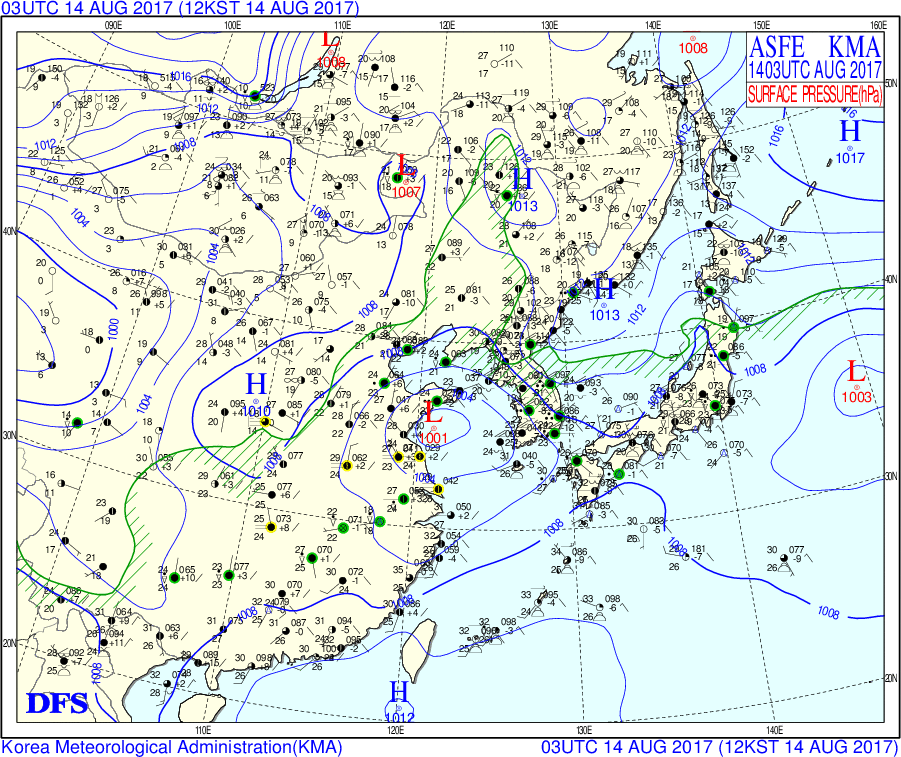
\includegraphics[width=0.97\linewidth]{22Weather_forecasting/images/sfc3_2017081403}
%%#	\caption{지상03 일기도(www.kma.go.kr)}
%%#	\label{fig:draw-weathermapsurf03}
%%#\end{figure}

\subsubsection{지상12}\index{지상12}
지상12 일기도는 00 UTC 기준 12시간 간격 (00, 12 UTC)으로 전 세계 동시에 작성한다. 각 관측소의 지상 기상 관측값을 볼 수 있고, 1,000 hPa 기준 4 hPa 간격으로 등압선을 그린다. 

\begin{figure}[p]\centering
	\begin{minipage}{0.97\textwidth}
	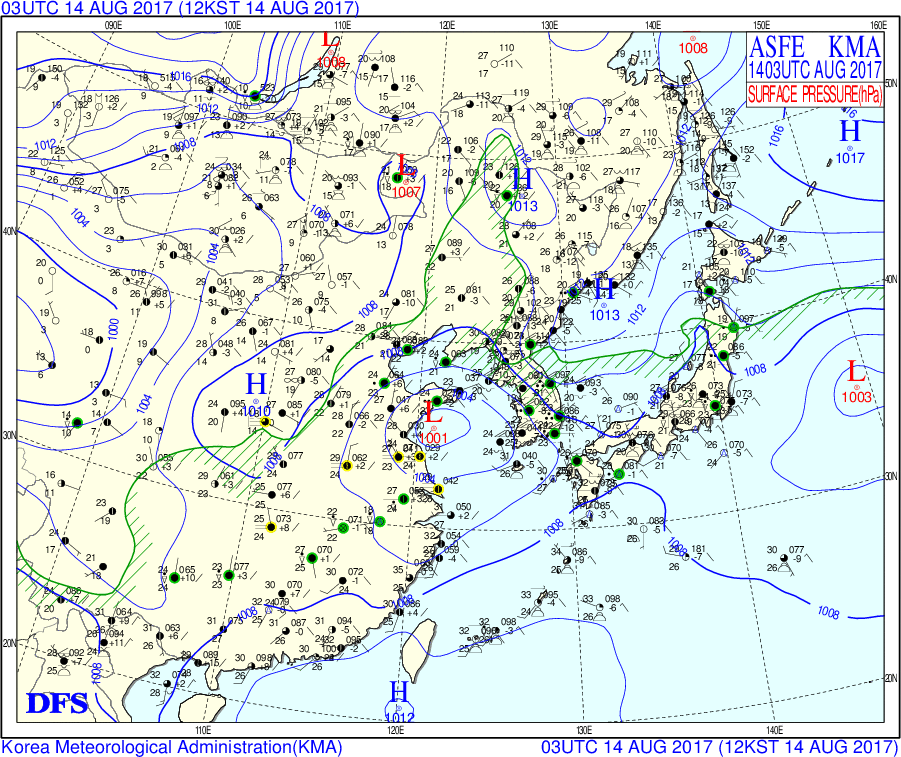
\includegraphics[width=0.97\linewidth]{22Weather_forecasting/images/sfc3_2017081403}
	\caption{지상03 일기도(www.kma.go.kr)}
\label{fig:draw-weathermapsurf03}
	\end{minipage}
	\begin{minipage}{0.97\textwidth}
	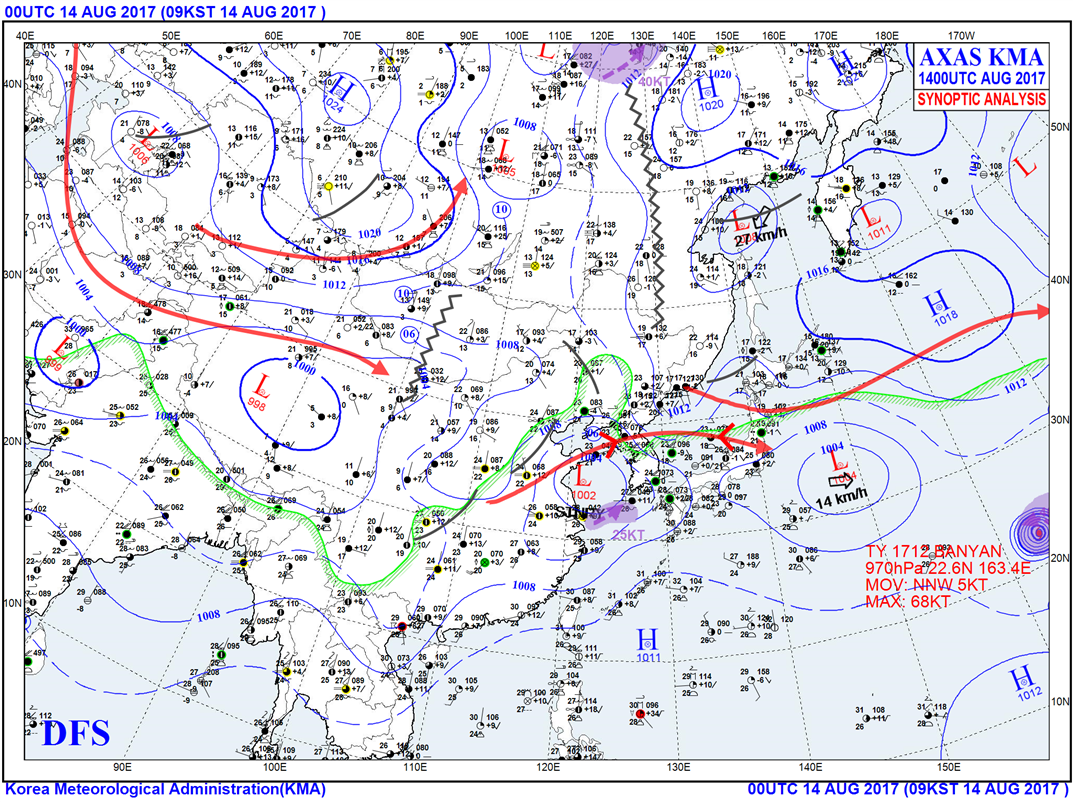
\includegraphics[width=0.97\linewidth]{22Weather_forecasting/images/surf_2017081400}
		\caption{지상12 일기도(www.kma.go.kr)}
		\label{fig:draw-weathermapsurf12}
	\end{minipage}
\end{figure}

\newpage
\subsection{상층 일기도}\index{상층 일기도}

상층의 등압면 고도, 기온, 풍속, 습도 등의 분포도를 말하며 고층 일기도라고도 한다. 고층의 일기 상태를 지상 일기도와 같이 평면적으로 나타낸 일기도이다. 기상청에서는 강수량 및 하층 대기의 기온 변화 예상에 필요한 925 hPa, 850 hPa, 700 hPa 일기도와 중층 대기에 대규모적인 기류 분석에 쓰이는 500 hPa 일기도, 대류권과 성층권 경계 부근의 제트기류 분석 등에 쓰이는 300 hPa (여름철에는 200 hPa), 항공기류 분석을 위해 100 hPa을 하루 두 번 (09시, 21시) 분석한다. 상층의 고기압과 저기압의 분포, 기단(기온) 분포, 건습(습도) 분포 등을 알아내는 데 이용된다.
%[네이버 지식백과] 상층일기도 [upper-air chart] (기상백과, 기상청)

\subsubsection{925 hPa 면 (810 m)}\index{925 hPa 면 (810 m)}
대류권의 최하층인 평균 810 m 높이의 기상 상황을 나타내는 상층 일기도이다. 각 관측소의 925 hPa 면의 상층 기상 관측값을 810 m기준 30 m 간격 등고선(청색 실선)과 3℃간격 등온선(적색 파선), 습윤 구역(노점 편차 < 2℃: 녹색 칠)로 나타낸다. 

\subsubsection{850 hPa 면 (1,500 m)}\index{850 hPa 면 (1,500 m)}
대기의 하층에 해당하는 지상 평균 1,500 m 높이의 상층 일기도로 지상 일기도와 대응시켜 사용되며, 전선 분석에 이용된다. 각 관측소의 850 hPa 면의 상층 기상 관측값을 1,500m기준 30m 간격 등고선(청색 실선)과 0℃ 기준 3℃간격 등온선(적색 파선), 습윤 구역(노점 편차 < 3℃: 녹색칠)을 나타낸다.

\subsubsection{700 hPa 면 (3,000 m)}\index{700 hPa 면 (3,000 m)}
대기의 하층에 해당하는 지상 평균 3,000 m 높이의 대류권 하층을 대표하는 고도의 상층 일기도로 수증기 분석에 적합하다. 각 관측소의 700 hPa 면의 상층 기상 관측값을 3,000 m 기준 60 m 간격 등고선(청색 실선)과 0℃ 기준 5℃ 간격 등온선(적색 파선), 습윤 구역(노점 편차 < 4℃: 녹색칠)을 나타낸다. 

\subsubsection{500 hPa 면 (5,580 m)}\index{500 hPa 면 (5,580 m)}
대기의 하층에 해당하는 지상 평균 5,580 m 높이의 대류권 중층(비발산 고도)으로 광범위한 대기 환류 조사에 적합하다. 각 관측소의 500 hPa 면의 상층 기상 관측값을 5,580 m 기준 60 m 간격 등고선(청색 실선)과 0℃ 기준 5℃ 간격 등온선(적색 파선) 나타낸다. 

\subsubsection{300 hPa 면 (9,180 m)}\index{300 hPa 면 (9,180 m)}
대류권의 상중층인 지상 평균 9,180 m 높이의 상층 일기도로 편서풍이 강하게 나타나며 제트류의 해석에 편리하다. 각 관측소의 300 hPa 면의 상층 기상 관측값을 9,180 m 기준 120 m 간격 등고선(청색 실선)과 0℃ 기준 5℃ 간격 등온선(적색 파선), 75 kt 기준 25 kt 간격의 등풍속선(녹색 실선), 강풍 구역(75 kts 이상 :  녹색점 집합), 제트기류 축(적색 띠 화살표)을 나타낸다. 

\subsubsection{200 hPa 면 (11,760 m)}\index{200 hPa 면 (11,760 m)}
대류권의 상층인 지상 평균 11,760 m 높이의 상층 일기도로 300hPa과 비슷하며 항공기에 대한 비행 정보 제공에 이용된다. 각 관측소의 200 hPa 면의 상층 기상 관측값을 11,760 m 기준 120 m 간격 등고선(청색 실선)과 0℃ 기준 5℃ 간격 등온선(적색 파선), 75 kt 기준 25 kt 간격의 등풍속선(녹색 실선), 강풍 구역(75 kts 이상 :  녹색점 집합), 제트기류 축(적색 띠 화살표)을 나타낸다. 

\subsubsection{100 hPa 면 (16,200 m)}\index{100 hPa 면 (16,200 m)}
대류권의 상층인 지상 평균 16,200 m 높이의 상층 일기도로 편서풍이 강하게 나타나며 제트류의 해석에 편리하다. 각 관측소의 100 hPa 면의 상층 기상 관측값을 16,200 m 기준 120 m 간격 등고선(청색 실선)과 0℃ 기준 5℃ 간격 등온선(적색 파선), 75 kt 기준 25 kt 간격의 등풍속선(녹색 실선), 강풍 구역(75 kts 이상 :  녹색점 집합), 제트기류 축(적색 띠 화살표)을 나타낸다. 

\begin{figure}[p]\centering
	\begin{minipage}{0.97\textwidth}
	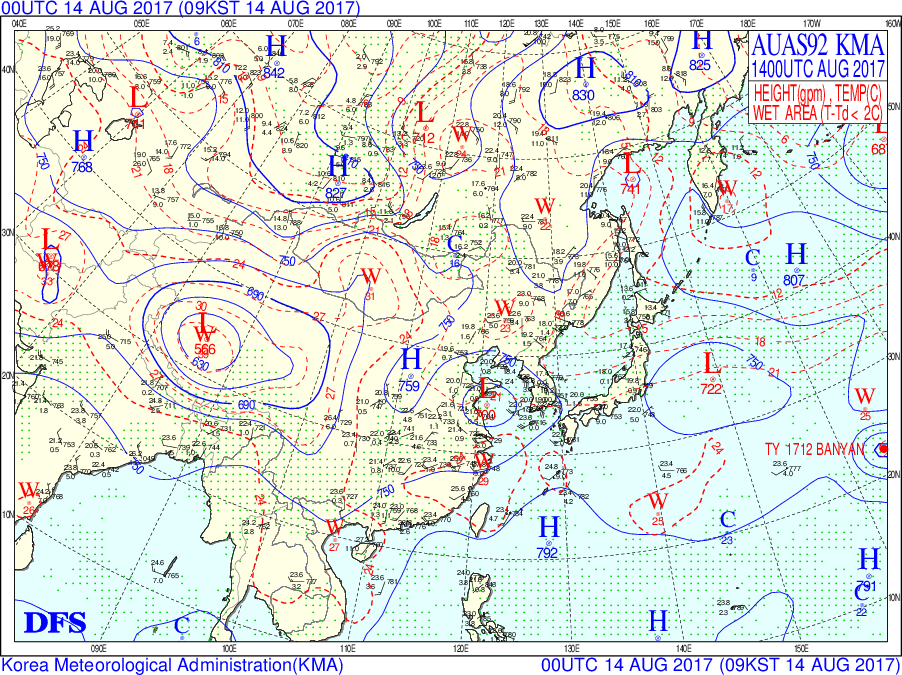
\includegraphics[width=0.97\linewidth]{22Weather_forecasting/images/up92_2017081400}
		\caption{925hPa 상층 일기도(www.kma.go.kr)}
		\label{fig:draw-weathermapsurf92}
	\end{minipage}
	\begin{minipage}{0.97\textwidth}
	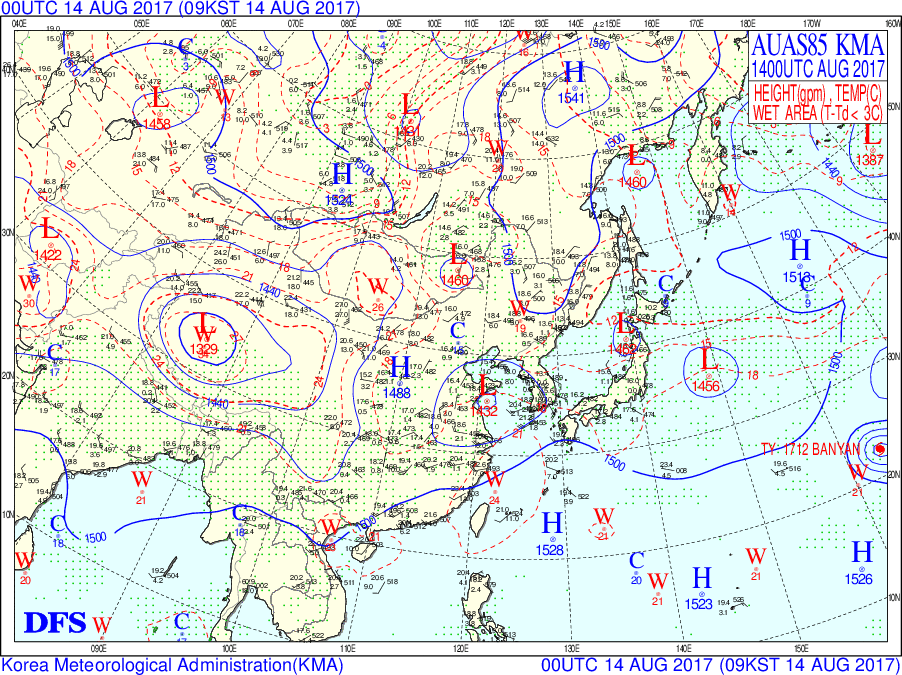
\includegraphics[width=0.97\linewidth]{22Weather_forecasting/images/up85_2017081400}
		\caption{850hPa 상층 일기도(www.kma.go.kr)}
		\label{fig:draw-weathermapsurf85}
	\end{minipage}
\end{figure}

\begin{figure}[p]\centering
	\begin{minipage}{0.97\textwidth}
	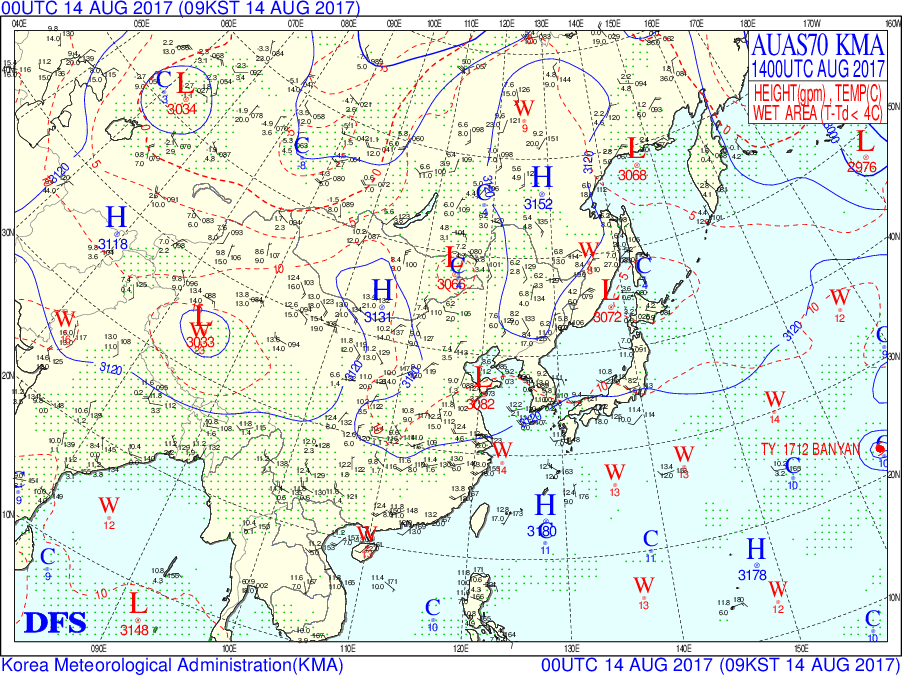
\includegraphics[width=0.97\linewidth]{22Weather_forecasting/images/up70_2017081400}
		\caption{700hPa 상층 일기도(www.kma.go.kr)}
		\label{fig:draw-weathermapsurf70}
	\end{minipage}
	\begin{minipage}{0.97\textwidth}
	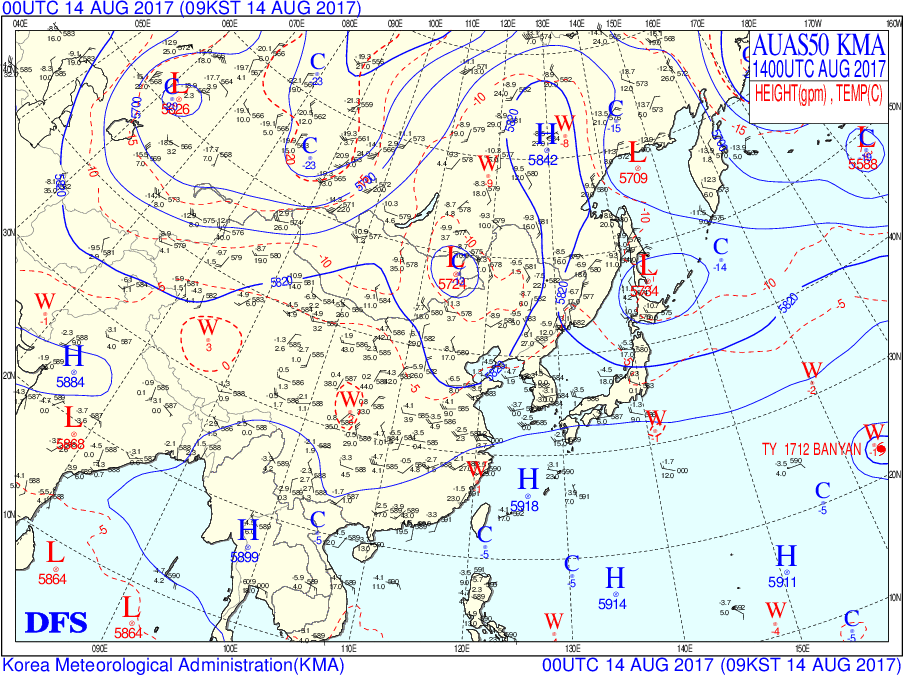
\includegraphics[width=0.97\linewidth]{22Weather_forecasting/images/up50_2017081400}
		\caption{500hPa 상층 일기도(www.kma.go.kr)}
		\label{fig:draw-weathermapsurf50}
	\end{minipage}
\end{figure}

\begin{figure}[p]\centering
	\begin{minipage}{0.97\textwidth}
	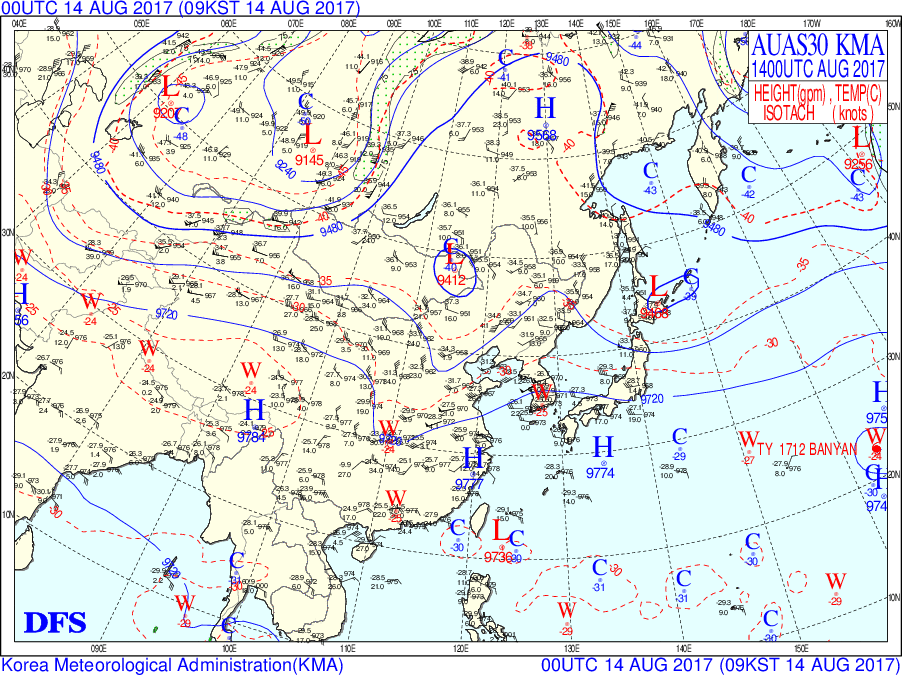
\includegraphics[width=0.97\linewidth]{22Weather_forecasting/images/up30_2017081400}
		\caption{300hPa 상층 일기도(www.kma.go.kr)}
		\label{fig:draw-weathermapsurf30}
	\end{minipage}
	\begin{minipage}{0.97\textwidth}
	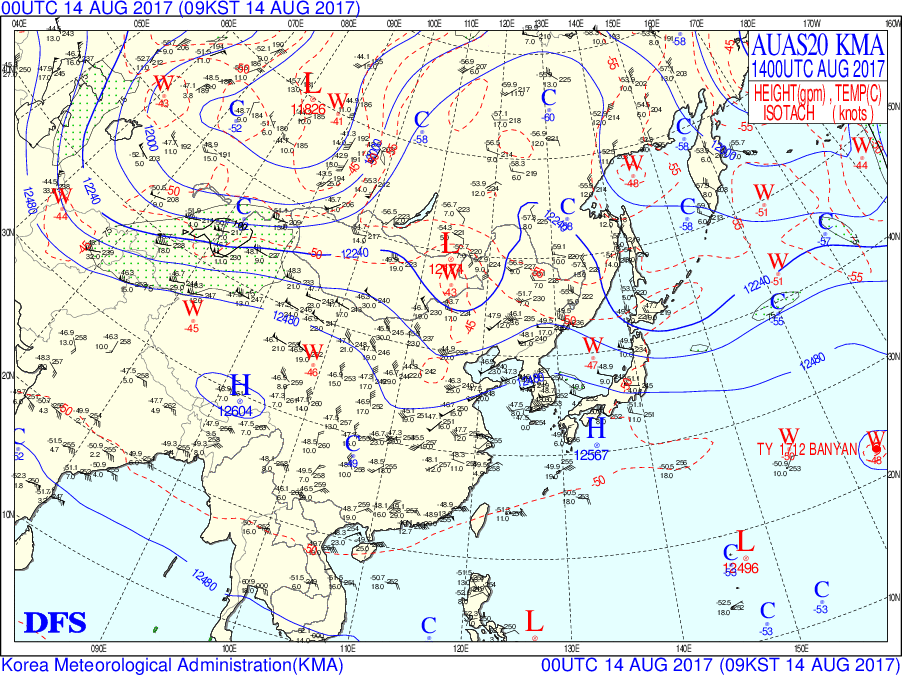
\includegraphics[width=0.97\linewidth]{22Weather_forecasting/images/up20_2017081400}
		\caption{200hPa 상층 일기도(www.kma.go.kr)}
		\label{fig:draw-weathermapsurf20}
	\end{minipage}
\end{figure}

\begin{figure}[h]\center
	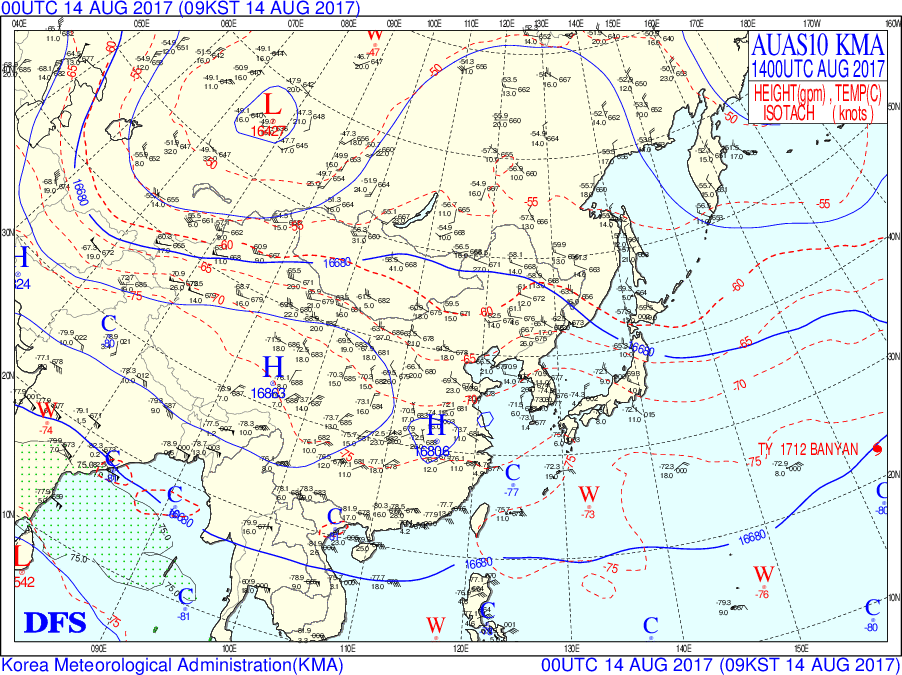
\includegraphics[width=0.97\linewidth]{22Weather_forecasting/images/up10_2017081400}
	\caption{100hPa 상층 일기도(www.kma.go.kr)}
	\label{fig:draw-weathermapsurf10}
\end{figure}


	

%%#\begin{itemize}
%%#	\item 925hPa면 일기도(810m) : 지상 일기도와 대응시켜 사용되며, 전선 분석에 이용된다.
%%#	\item 850hPa면 일기도(1,500m) : 지상 일기도와 대응시켜 사용되며, 전선 분석에 이용된다.
%%#	\item 700hPa면 일기도(3,000m) : 대류권 하층을 대표로 하는 고도로 수증기 분석에 적합하다.
%%#	\item 500hPa면 일기도(5,580m) : 대류권 중층(비발산 고도)으로 광범위한 대기 환류 조사에 적합하다.
%%#	\item 300hPa면 일기도(9,180m) : 대류권 상층으로 편서풍이 강하게 나타난다. 제트류의 해석에 편리하다.
%%#	\item 200hPa면 일기도(11,760m) : 300hPa과 비슷하며 항공기에 대한 비행 정보 제공에 이용된다.
%%#\end{itemize}

%%#\begin{figure}[!htb]\centering
%%#	\begin{minipage}{0.49\textwidth}
%%#		\frame{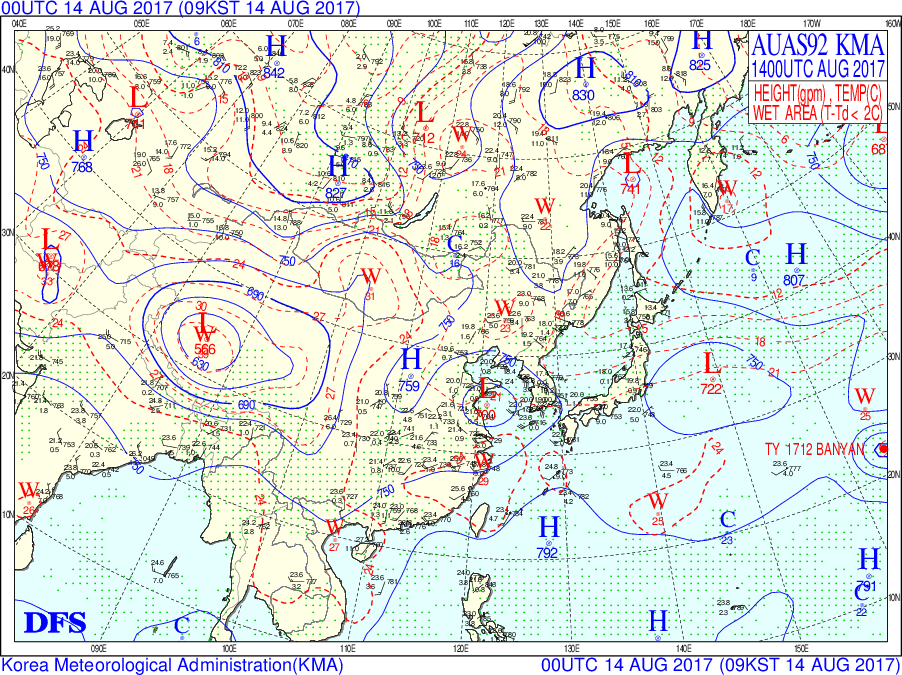
\includegraphics[width=0.95\linewidth]{22Weather_forecasting/images/up92_2017081400}}
%%#	\caption{925hPa 상층 일기도(www.kma.go.kr)}
%%#	\label{fig:draw-weathermapsurf92}
%%#	\end{minipage}
%%#	\begin {minipage}{0.49\textwidth}
%%#	\frame{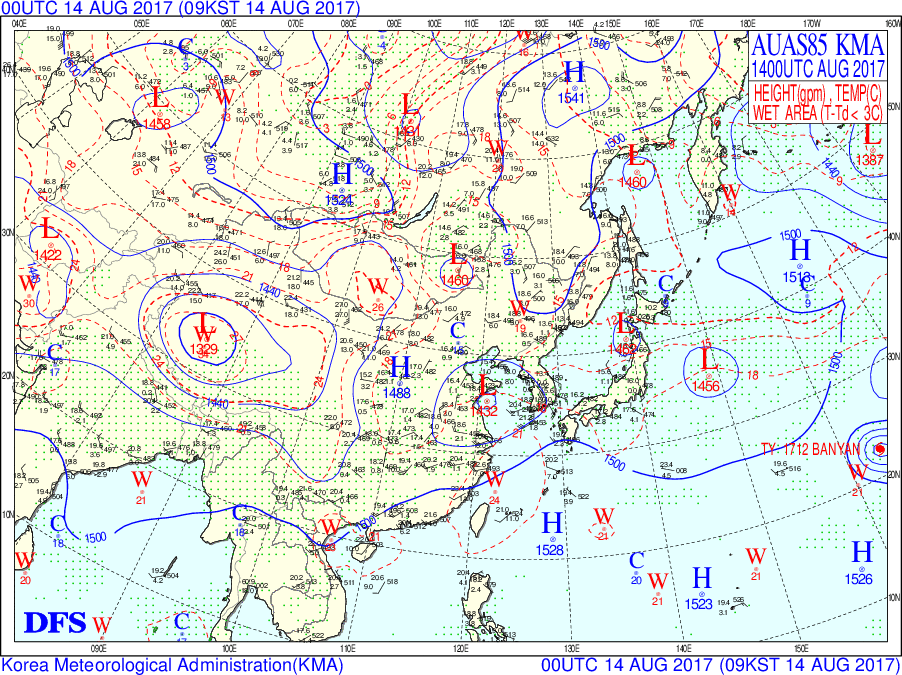
\includegraphics[width=0.95\linewidth]{22Weather_forecasting/images/up85_2017081400}}
%%#		\caption{850hPa 상층 일기도(www.kma.go.kr)}
%%#		\label{fig:draw-weathermapsurf85}
%%#	\end{minipage}
%%#\end{figure}


\newpage
\section{일기도 그리기}\index{일기도 그리기}

\subsection{기상 관측}\index{관측 자료 기입}
지상 혹은 상층 대기 상태를 요소별로 관측하는 것으로 관측 자료는 기상 예보 판단의 기본 요소가 된다.

\begin{itemize}
	\item 지상 관측: 운고, 운량, 운형, 시정, 기상 현상, 기압, 이슬점, 습도, 풍향, 풍속, 강수량, 적설량 및 기타 특수 현상을 목측 혹은 계기에 의해 관측하는 것을 말한다.
	\item 고층 기상 관측: 상층 고도별 풍향, 풍속, 기온, 이슬점 온도, 습도, 기압을 계기에 의해 측정한다.
	\item 상층풍 관측 : 상층의 고도별 풍향·풍속을 기구를 비양시켜 측정한다.
	\item 그 외에 레이더 관측, 항공기 관측, 위성 관측 등이 있다.
\end{itemize}


\subsection{기상 전문 기입}\index{기상 전문 기입}

WMO에서 지정한 각 지점에 주어진 시간의 기상 전문을 수신하여 일기도 각 지점에 기입해야 하는데, 일기도에 관측된 자료를 나타낼 때에는 \ref{fig:drawsymbols-1}\과 같이 정해진 형식으로 기입해야 한다. 단 예시에서 기온은 화씨임에 유의하라.

\begin{figure}[p]
	\centering
	\includegraphics[width=0.95\linewidth]{22Weather_forecasting/images/wxsymbol_print-1}
	\caption{일기도 기호 기입 형식(NOAA)}
	\label{fig:drawsymbols-1}
\end{figure}

\begin{figure}[p]
	\centering
	\includegraphics[width=0.95\linewidth]{22Weather_forecasting/images/wxsymbol_print-2}
	\caption{일기도 기호 기입 형식(NOAA)}
	\label{fig:drawsymbols-1}
\end{figure}

%%#\begin{figure}[p]
%%#	\centering
%%#	\includegraphics[width=0.95\linewidth]{22Weather_forecasting/images/wxsymbol_print-12}
%%#	\caption{일기도 기호 기입 형식(NOAA)}
%%#	\label{fig:drawsymbols}
%%#\end{figure}

\newpage
\subsection{등압선 그리는 방법}\index{등압선 그리는 방법}
일기도에서 가장 중요하게 다루는 선이 등압선이다. 등압선은 기압이 같은 지점을 연결한 선이다. 등압선을 그려 보면 고기압과 저기압의 위치, 전선 등을 가려 낼 수 있다. 이것은 마치 지도에 그려진 등고선의 분포 모양을 보고 산이나 골짜기를 판별하는 것과 유사하다. 

등압선은 다음과 같은 방법으로 그린다.
\begin{enumerate}
 \item 주어진 일기도에 기입된 각종 자료 중 구름의 양, 풍향, 풍속, 기압 등의 의미를 파악한다. 
 \item 해면 기압은 자연 상태에서 보통 1060 hPa을 넘지 않으므로, 첫자리 수가 0에서 5사이이면 10을, 6과 9사이 이면 9를 각각 앞에 붙여 계산한다.
 \item 일반적으로 등압선은 1000 hPa을 기준으로 ......, 992, 996, 1000, 1004, 1008, ...... 등 4 hPa 간격으로 그린다. 그러나 등압선 간의 폭이 너무 넓어 기압배치를 파악하기 어려울 때는 2 hPa 간격으로 파선을 그린다.
 \item 그리기 쉬운 곳(등압선이 조밀하지 않은 곳)부터 그려 나간다.
 \item 등압선은 중간에서 끊어지거나 없어지지 않는다.
 \item 관측값이 없는 경우는 내삽, 또는 외삽법의 원리로 \ref{fig:drawweathermap01}\과 같이 이웃하는 두 지점의 간격을 비례로 나누어서 부드럽고 매끈한 곡선으로 그린다.
 \item 한 선으로 연결되는 등압선은 양쪽 끝에 기압의 값을 기입하고, 폐곡선의 경우는 위쪽(북쪽) 중앙에 등압선을 끊고 값을 기입한다. 
 \item 저기압의 중심은 적색으로 L(low pressure), 고기압의 중심은 청색으로 H(high pressure)라고 표시한다.
\end{enumerate}

\begin{figure}[h]
	\centering
	\includegraphics[width=0.8\linewidth]{22Weather_forecasting/images/draw-weathermap01}
	\caption{등압선의 작도 방법}
	\label{fig:drawweathermap01}
\end{figure}

등압선을 그리고 나면 고기압과 저기압의 위치 및 이동경로, 기압과 고도의 변화경향, 전선의 발생 및 소멸과 이동, 날씨 변화, 대기의 수직 구조 등을 세밀히 분석하게 된다. 

전선의 위치를 찾는 방법은 다음과 같다.

\begin{enumerate}
 \item 전선은 기온, 이슬점, 풍향이 불연속을 이루므로 이들 값이 급변하는 지역을 찾는다.
 \item 전선 근처에서는 일반적으로 일기가 악화되므로 강수 등의 일기가 선상으로 나타날 경우 전선이 존재할 가능성이 높다. 
 \item 온난전선은 전면의 넓은 지역에서 강수 현상이 나타나고 후면에는 비교적 맑은 날씨를 이룬다. 한랭전선은 전면과 후면의 구별 없이 전선 상에서 비교적 좁은 지역에 강수 현상이 나타난다.
 \item 전선이 확인되면 \ref{fig:drawweathermap02}\와 같이 등압선이 휘도록 연결한다.
\end{enumerate}

\begin{figure}[h]
	\centering
	\includegraphics[width=0.8\linewidth]{22Weather_forecasting/images/draw-weathermap02}
	\caption{전선에서의 등압선}
	\label{fig:drawweathermap02}
\end{figure}

\newpage
\subsection{실습 에제}\index{실습 예제}
다음 일기도에 등압선을 그리고 고기압, 저기압의 위치 및 전선을 찾아 표시해 보자.

\subsubsection{전선이 그려진 경우}\index{전선이 그려진 경우}

\begin{figure}[h]\center
	\centering
	\includegraphics[width=1.0\linewidth]{22Weather_forecasting/images/isobar_ex01}
%	\caption{}
	\label{fig:isobar_ex01}
\end{figure}

\newpage
\subsubsection{전선이 한 개 있는 경우}\index{전선이 한개 있는 경우}

\begin{figure}[h]\center
	\centering
	\includegraphics[width=1.0\linewidth]{22Weather_forecasting/images/isobar_ex02}
	%	\caption{}
	\label{fig:isobar_ex02}
\end{figure}

\newpage
\subsubsection{전선이 두 개 있는 경우}\index{전선이 두 개 있는 경우}

\begin{figure}[h]\center
	\centering
	\includegraphics[width=1.0\linewidth]{22Weather_forecasting/images/isobar_ex03}
	%	\caption{}
	\label{fig:isobar_ex03}
\end{figure}

\newpage
\subsubsection{등압선 그리기}\index{등압선 그리기}

\begin{figure}[h]\center
	\centering
	\includegraphics[width=1.0\linewidth]{22Weather_forecasting/images/surf_pltstn_pbg_2004122400}
	\caption{등압선 그리기 예제}
	\label{fig:drawweathermap03}
\end{figure}


\chapterimage{chapter_head_1.pdf} % Chapter heading image
\chapter{기상청 일기 예보}

\section{예보가 나오는 과정}

예보가 나오기까지는 기상실황파악 → 자료수집 → 분석 → 예보작성 → 통보 과정을 거친다. 

\section{기상실황 파악}

\subsection{지상기상 관측}
전국 76개소의 기상관서에서 하늘상태, 시정 등의 목측 (目測 ) 요소를 관측하고 있으며, 기온, 습도, 강수량, 바람, 기압 등은 자동기상관측장비를 이용하여 1분 간격으로 관측되고 있다. 또한, 기상관서가 없는 500여 소에서는 방재용 자동기상관측장비를 이용하여 기온, 풍향, 풍속, 강수량, 강수 유무를 1분 간격으로 관측하여 기상실황을 감시하고 있다.

\subsection{항공기상관측}
전국 공항기상관서에서는 바람, 시정, 운고, 기온, 기압 등의 항공기상관측요소를 매30분 또는 1시간 간격으로 관측하며, 활주로에 설치된 공항기상관측장비에 의해 기상요소들이 매분 자동 관측된다. 특히 인천, 제주, 양양, 울산 등의 공항에서는 이·착륙 항공기에 영향을 미치는 저층난류를 탐측하기 위하여 저층난류경보장치를 운영하고 있다.

\subsection{고층기상관측}
고층기상관측은 지상보다 높은 상층 대기의 상태를 관측하는 것으로, 기상청은 레윈존데 관측, 수직측풍장비 관측을 수행한다. 레윈존데 관측은 기구에 라디오존데를 매달아 지상으로부터 약 35 km(5 hPa)까지의 고도별 기압, 기온, 습도, 풍향, 풍속을 00UTC와 12UTC에 관측하며, 수직측풍장비 관측은 UHF나 VHF 파장의 전파를 상층대기로 방사하고 바람과 함께 이동하는 난류에 산란되어 다시 수신되는 전파신호로 바람을 10분 간격으로 관측한다.

\subsection{해양기상관측}
해양기상관서, 해양기상관측부이, 해양기상영상감시시스템을 통하여 풍향·풍속, 기온, 수온, 기압, 파고 등을 관측하며, 먼바다의 기상현상 관측 및 부이 관리를 위하여 기상관측선을 운영하고 있다.

\subsection{기상위성관측}
기상위성은 우주공간에서 지구의 기상변화를 관측한다. 기상청은 정지궤도기상위성과 극궤도기상위성의 자료를 직접 수신하여 처리하여 예보를 위해 사용하고, 국민에게도 공개하고 있다. 이를 위해 기상위성 수신처리분석시스템을 서울, 문산, 서산에 설치하여 운영중이다.

\subsection{기상레이더 관측}
도플러 기상레이더를 설치하여 한반도에서 발생하는 악기상을 관측하여 예보에 활용하고 있다. 또한 일본 기상청과 공군의 레이더 자료도 수신하여 기존영상과 합성하여 종합적으로 활용하고 있다.


\section{자료수집}
통신용컴퓨터를 이용하여 국내기상자료와 외국에서 송신되는 각종기상자료를 수집, 편집, 가공하여 분석용 컴퓨터로 보낸다. 국내·외에서 수집된 관측자료로부터 수치예보모델을 이용하여 예상일기도를 생산한다. 이러한 수치예보모델의 운용을 위해 슈퍼컴퓨터가 사용된다.



\section{일기도 그리기}\index{일기도 그리기}

\subsection{일기도}\index{일기도}
일기도(지상 일기도)는 어느 지역 내의 일기 개황을 한 눈에 보아서 알 수 있도록
각종 기상요소(기압, 습도, 기온, 이슬점, 운량, 풍향, 풍속 등)를 나타낸 것으로 이것을
이용하여 각 지역의 일기를 알 수 있으며, 연속된 일기도를 통해 앞으로의 일기를 예상할 수 있다.

\subsection{관측자료 기입}\index{관측자료 기입}
일기도에 관측된 자료를 나타낼 때에는 <그림 Ⅲ-20>과 같이 정해진 일정한 형식으로 기입해야 한다. 기입이 끝나면 일기도 상에서 기압, 기온 또는 필요한 기상요소들에 대하여 값이 같은 점을 연결하여 선을 긋는다. 일기도에서 가장 중요하게 다루는 선이 등압선이다. 등압선은 기압이 같은 지점을 연결한 선이다. 등압선을 그려보면 고기압과 저기압의 위치, 전선 등을 가려 낼 수 있다. 이것은 마치 지도에 그려진 등고선의 분포모양을 보고 산이나 골짜기를 판별하는 것과 유사하다. 등압선을 그리는 방법은 다음과 같다.
① 주어진 일기도에 기입된 각종 자료 중 구름의 양, 풍향, 풍속, 기압 등의 의미를 파악한다.
기압은 자연 상태에서 보통 1060 hPa을 넘지 않으므로, 첫자리 수가 0에서 5사이이면 10
을, 6에서 9사이이면 9를 각각 앞에 붙여 계산한다.
② 일반적으로 등압선은 1000 hPa을 기준으로 ......, 992, 996, 1000, 1004, 1008, ...... 등 4 hPa 간격으로 그린다. 그러나 등압선 간의 폭이 너무 넓어 기압배치를 파악하기 어려울
때는 2 hPa 간격으로 파선을 그린다.
③ 그리기 쉬운 곳(등압선이 조밀하지 않은 곳)부터 그려 나간다.
④ 등압선은 중간에서 끊어지거나 없어지지 않는다.
⑤ 관측값이 없는 경우는 내삽, 또는 외삽법의 원리로 <그림 Ⅲ-21>과 같이 이웃하는 두 지
점의 간격을 비례로 나누어서 부드럽고 매끈한 곡선으로 그린다.
⑥ 한 선으로 연결되는 등압선은 양쪽 끝에 기압의 값을 기입하고, 폐곡선의 경우는 위쪽(북
쪽) 중앙에 등압선을 끊고 값을 기입한다. 저기압의 중심은 적색으로 L(low pressure), 고
기압의 중심은 청색으로 H(high pressure)라고 표시한다.
일기도가 그려지면 고기압과 저기압의 위치 및 이동경로, 기압과 고도의 변화경향, 전선의
발생 및 소멸과 이동, 날씨변화, 대기의 수직구조 등을 세밀히 분석하게 된다. 전선의 위치를
찾는 방법은 다음과 같다.
\begin{figure}
	\centering
	\includegraphics[width=0.8\linewidth]{Pictures/draw-weathermap01}
	\caption{등압선의 작도 방법}
	\label{fig:draw-weathermap01}
\end{figure}법

① 전선은 기온, 이슬점, 풍향이 불연속을 이루므로 이들 값이 급변하는 지역을 찾는다.
② 전선 상에서는 일반적으로 일기가 악화되므로 강수 등 나쁜 일기가 선상으로 나타날 경
우 전선이 존재할 가능성이 높다. 온난전선은 전면의 넓은 지역에서 강수 현상이 나타나
고 후면에는 비교적 맑은 날씨를 이룬다. 한랭전선은 전면과 후면의 구별 없이 전선 상에
서 비교적 좁은 지역에 강수 현상이 나타난다.
③ 전선이 확인되면 <그림 Ⅲ-22>와 같이 등압선이 휘도록 연결한다.

\begin{figure}
	\centering
	\includegraphics[width=0.8\linewidth]{Pictures/draw-weathermap02}
	\caption{전선에서의 등압선}
	\label{fig:draw-weathermap02}
\end{figure}



일기도 그리기
여러 가지 기상요소 중 간단한 등압선을 그리고 고·저기압의 위치 및 전선을 찾아 일기도를 완성해 보자.




\section{Corollaries}\index{Corollaries}

This is an example of a corollary.

\begin{corollary}[Corollary name]
	The concepts presented here are now in conventional employment in mathematics. Vector spaces are taken over the field $\mathbb{K}=\mathbb{R}$, however, established properties are easily extended to $\mathbb{K}=\mathbb{C}$.
	end{corollary}
	
	%------------------------------------------------
	
	\section{일기도 분석}\index{일기도 분석}
	
	기온, 강수 유무 등의 매일의 일기는 산업과 일상생활에 많은 영향을 미친다. 따라서 오랜
	세월 동안 일기를 정확히 예측하고자 많은 노력을 기울여 왔다. 아직도 많은 한계를 안고 있으
	나 날씨는 갑자기 변하는 것이 아니고 과거로부터 연속성을 가지고 변화하므로 과거와 현재의
	일기상태를 분석함으로써 미래의 일기를 어느 정도 예측할 수 있으며 보다 정확한 예측을 위
	하여 노력을 계속하고 있는 실정이다.
	일기의 분포는 일반적으로 기압배치에 대응되므로 기압배치를 예상할 수 있으면 일기예보
	가 어느 정도 가능하다. 고기압, 저기압의 기압계는 지속성을 가지고 있고, 우리나라 주변에서
	는 서에서 동으로 이동하므로 이를 이용하여 앞으로의 기압배치를 예측하고 날씨를 예상할 수
	있다. 고기압이 있는 지역의 지상일기는 하강 기류로 인해 구름이 소멸되어 맑은 날씨를 나타
	낸다. 반면 저기압지역에서는 내부의 상승기류로 인해 구름이 만들어지고 비가 내리게 되어
	궂은 날씨가 된다. 저기압은 전선을 동반하는 경우도 있는데 전선은 성질이 다른 두 기단의 경
	계를 이루는 상대적으로 좁은 영역을 이루므로 이 영역을 기준으로 온도나 바람 등이 급변할
	뿐 아니라 일반적으로 일기가 악화되어 강수 현상 등이 나타난다.
	
	\begin{figure}
		\centering
		\includegraphics[width=0.8\linewidth]{Pictures/weathermap01}
		\caption{태풍이 이동하는 일기도}
		\label{fig:weathermap01}
	\end{figure}
	
	
	실제로 일기도가 완성되면 예보관은 이를 다각적으로 분석한다. 일기도의 분석은 고기압과
	저기압의 위치 및 이동경로, 기압과 고도의 변화경향, 전선의 발생 및 소멸과 이동 추적, 날씨
	변화, 대기의 연직구조 등을 세밀히 분석한다. 또한 특수기상 관측 자료인 기상레이더에 의한
	강수구역 추적, 기상위성에 의한 구름사진 분석, 자동기상관측자료(AWS) 등을 분석하여 앞으
	로의 날씨변화를 예상하게 된다. 또한 최근에는 컴퓨터를 활용하여 짧은 시간에 많은 기상자
	료를 처리할 수 있게 됨으로써 수치분석자료와 각종 보조일기도들을 이용할 수 있게 되어 정
	확한 날씨를 판단하는데 많은 도움을 주고 있다.
	
	\subsection{예상일기도 그리기}\index{Propositions!Several Equations}
	
	연속적인 몇 장의 일기도를 분석하여 앞으로 전개될 대기 상태를 예측하여 예상 일기도를 그려 보자.
	
	1. <그림 1>~<그림 4>는 2007년 7월 1일 6시부터 2일 18시까지 12시간 간격으로 연속 4회 동안 관
	측하여 작성한 지상일기도이다.
	⑴ 일기도 상에 나타난 전선을 다음 그림에 그려 넣고, 전선이 어느 방향으로 얼마나 이동했으며 평
	균 이동 속도는 얼마인지 다음 표를 작성하라. (단, 경도 1°의 거리는 위도 30°에서 96.5 km, 위도
	40°에서 85.4 km, 위도 50°에서 71.7 km이다. 위도 1°사이의 거리는 약 110 km이다.)
	
	
	⑵ 7월 3일 6시에는 기압계가 어떻게 달라졌을지 예상하여 다음 그림에 예상 일기도를 그려 보자.
	
	⑶ 다음 표는  기상청에서 발표한 7월 1일과 2일의 예보 통보문이다. 그린 예상 일기도를 바탕으로 예보 통보문을 작성해 보자.
	
	\begin{tabular}{|c|c|}
		\hline 
		일시	& 예보 통보문 \\ 
		\hline 
		7월 1일	& 동해상에 위치한 고기압 가장자리에 들겠습니다.
		전국이 대체로 구름 많고, 경상북도 지방은 새벽까지, 전라남북도 지방에서 아침까지 소
		나기(강수확률 60{\%})가 오는 곳이 있겠고, 오후에는 대기불안정으로 남부 내륙지방을 중
		심으로 산발적으로 소나기(강수확률 60{\%}가 오는 곳이 있겠습니다. \\ 
		\hline 
		7월 2일	& 서쪽에서 접근하는 장마전선의 영향을 점차 받겠습니다.
		전국이 대체로 흐리고 새벽에 중부서해안지방부터 비(강수확률 60~ 90{\%}가 시작되어 밤
		에는 전국으로 확대되겠습니다. \\ 
		\hline 
		7월 3일	&  \\ 
		\hline 
	\end{tabular} 





%----------------------------------------------------------------------------------------
%	CHAPTER 
%----------------------------------------------------------------------------------------

\chapterimage{chapter_head_1.pdf} % Chapter heading image

\chapter{기상청(www.kma.go.kr) 일기 예보}

\section{기상청 일기 예보의 종류}


\subsection{초단기 동네 예보}
초단기예보는 현재부터 앞으로 3시간까지, 실황(날씨, 기온, 습도 등 7개 요소)과 예보(강수형태, 하늘상태, 강수량 등 3개 요소)를 1시간 간격으로 동네예보를 기반으로 매 시각 30분에 발표한다. 초단기예보는 짧은 시간에 발생·소멸하는 기상현상에 대해 신속하게 대응하여 재해예방에 최선을 다하고자 2010년 6월 15일부터 홈페이지를 통해 제공하고 있다.

\subsection{동네 예보}
대상기간과 구역을 시ㆍ공간적으로 세분화하여 발표하는 예보로 기온, 최고기온, 최저기온, 강수형태, 강수확률, 12시간강수량, 12시간적설, 하늘상태, 습도, 풍향, 풍속, 파고 등을 예보한다. 동네예보는 3시간 간격으로 1일에 8회 예보하며 예보구간도 역시 3시간 단위로 48시간까지 예보한다. 

\subsection{주간 예보}
기상전망, 예보구역별 육상 및 해상 날씨, 지점별 기온, 파고에 대한 48시간 이후부터  6일간의 예보로 일 2회 발표(06시, 18시)하는 주간예보(모레부터 6일간)가 계속 유지될 가능성에 대한 신뢰도 정보를 3단계로 구분하여 제공(육상)한다.

\begin{table}[h]
	\centering
	\caption{신뢰도와 의미}
	\begin{tabular*}{.8\linewidth}{c|c}
		\hline 
		신뢰도  &	내용	  \\ 	\hline 
		높음  & 다음날 발표 주간예보가 계속 유지될 가능성이 높음  \\  \hline 
		보통 & 다음날 발표 주간예보가 계속 유지될 가능성이 있음  \\ 	\hline 
		낮음 & 다음날 발표 주간예보가 계속 유지될 가능성이 낮음   \\ 	\hline 
	\end{tabular*} 
\end{table}

\subsection{주말 예보}
토요일과 일요일의 기상 개황, 일별 날씨, 야외활동 지수 등의 정보를 제공한다. 화요일 19시부터 금요일 24시까지 제공되며, 매일 19시에 발표한다.

\subsection{장기 예보}
장기예보는 11일 이상에 대한 예보를 일컬으며 순별·월별 기압계 동향 및 전망, 기온·강수량 예보 등을 발표한다. 예보구역은 한반도 12개 권역(서울·인천·경기도, 강원도 영서, 강원도 영동, 대전·충청남도, 충청북도, 광주·전라남도, 전라북도, 부산·울산·경상남도, 대구·경상북도, 제주도, 평안남북도·황해도, 함경남북도)이며, 월 3회 발표되는 1월 전망과 월 1회 발표되는 3개월 전망이 있다. 그 외 연 4회 발표되는 기후전망은 다음다음 계절에 대한 전망으로 봄철 기후전망은 11월 23일 경에, 여름철 기후전망은 2월 23일 경에, 가을철 기후전망은 5월 23일 경에 겨울철 기후전망은 8월 23일 경에 발표한다.



\section{기상 위성 자료의 해석}

\subsection{기상위성의 이해}\index{기상위성의 이해}


\chapterimage{chapter_head_1.pdf} % Chapter heading image

\chapter{컴퓨터 활용}

\section{일기도 그리기}

\subsection{지도 그리기}\index{지도 그리기}

Figure \ref{fig:mapofkorea01} \과 같은 지도를 그려보자.
\begin{figure}[h]
	\centering
	\includegraphics[width=0.7\linewidth]{MapOfKorea01}
	\caption{한반도 주변 지도(메르카토르도법)}
	\label{fig:mapofkorea01}
\end{figure}


\begin{code}[한반도 주변 지도(메르카토르도법)]
	\begin{lstlisting}
	
	#python 
	from mpl_toolkits.basemap import Basemap
	import matplotlib.pyplot as plt
	import numpy as np
	
	# create new figure, axes instances.
	fig = plt.figure()
	ax = fig.add_axes([0.1,0.1,0.8,0.8])
	
	#loglat = [west,south,east,north]
	loglat = [111,25,145,50]
	clog = (loglat[2]+loglat[0]) / 2
	clat = (loglat[3]+loglat[1]) / 2
	
	#map projection.
	m = Basemap(llcrnrlon=loglat[0],llcrnrlat=loglat[1],\
	urcrnrlon=loglat[2],urcrnrlat=loglat[3],\
	rsphere=(6378137.00,6356752.3142),\
	resolution='l',projection='merc',\
	lon_0=clog,lat_0=clat,lat_ts=20.)
	
	m.drawcoastlines()
	m.drawcountries()
	m.fillcontinents()
	
	# draw parallels
	m.drawparallels(np.arange(10,90,10),labels=[1,1,0,1])
	# draw meridians
	m.drawmeridians(np.arange(-180,180,10),labels=[1,1,0,1])
	
	plt.show()
	
	\end{lstlisting}
\end{code}

\subsection{일기도 모양의 지도 그리기}\index{일기도 모양의 지도 그리기}

Figure \ref{fig:surf201707021} \은 기상청(http://www.kma.go.kr/weather/images/analysischart.jsp)에서 제공하는 지상일기도이다. 

\begin{figure}[h]
	\centering
	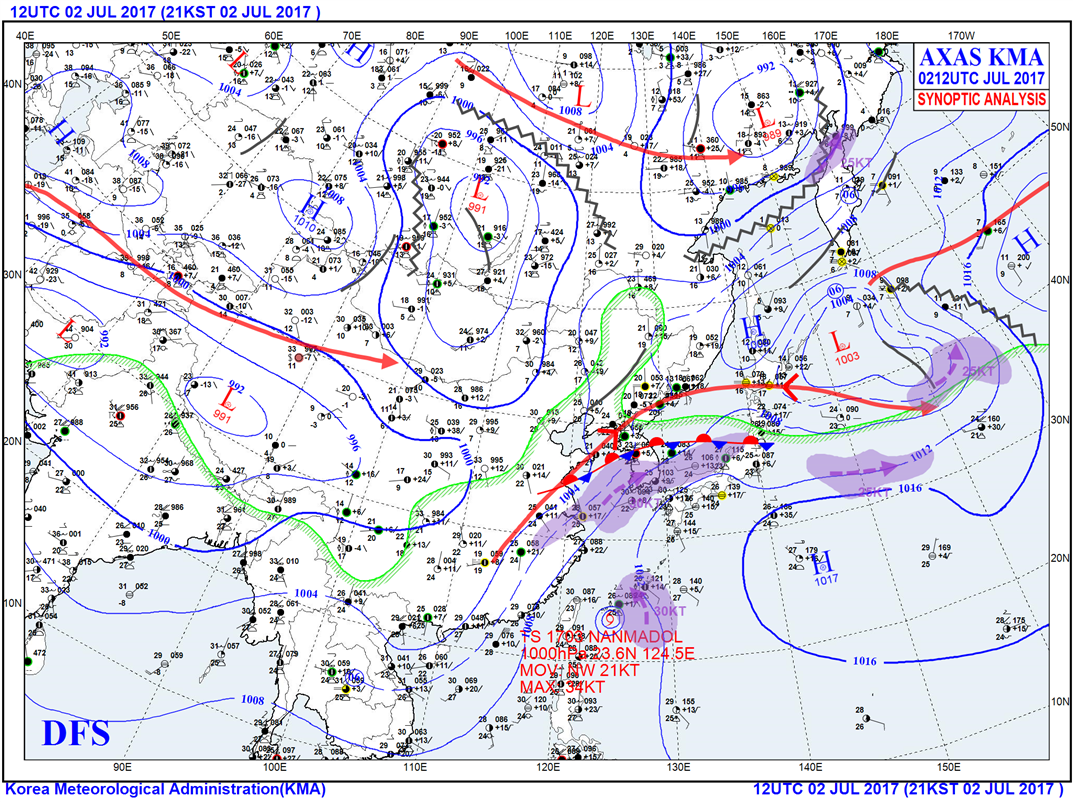
\includegraphics[width=0.8\linewidth]{surf_2017070212}
	\caption{기상청 지상일기도}
	\label{fig:surf2017070212}
\end{figure}

이와 비슷한 지도를 그리는 코드틑 다음과 같다.

\begin{code}[기상청 일기도모양 백지도]
	%	\begin{align}
	\begin{lstlisting}
	
	from mpl_toolkits.basemap import Basemap
	#python 
	import matplotlib.pyplot as plt
	import numpy as np
	
	# create new figure, axes instances.
	fig=plt.figure()
	ax=fig.add_axes([0.1,0.1,0.8,0.8])
	
	#loglat = [west,south,east,north]
	loglat = [90,0,180,62]
	clog = (loglat[2]+loglat[0])/2
	clat = (loglat[3]+loglat[1])/2
	
	# map projection.
	m = Basemap(llcrnrlon=loglat[0],llcrnrlat=loglat[1],\
	urcrnrlon=loglat[2],urcrnrlat=loglat[3],\
	resolution='l',projection='aea',lon_0=clog,lat_0=clat)
	
	m.drawcoastlines()
	m.drawcountries()
	m.fillcontinents()
	
	# draw parallels
	m.drawparallels(np.arange(0,90,10),labels=[1,1,0,0])
	# draw meridians
	m.drawmeridians(np.arange(-180,180,20),labels=[0,0,1,0])
	m.drawmeridians(np.arange(-180,180,10),labels=[0,0,0,1])
	
	plt.show()	
	\end{lstlisting}
	%		\end{align}
\end{code}

그 결과이다. 

\begin{figure}[h]
	\centering
	\includegraphics[width=0.8\linewidth]{weathermap01}
	\caption{기상청 일기도모양 백지도}
	\label{fig:weathermap01}
\end{figure}
\section{지구 온난화 모델링}

\subsection{Time-Stepping Naked Planet Model}\index{Time-Stepping Naked Planet Model}

\subsubsection{How the Model Works}\index{}

So the naked planet model is an energy balance model. We have energy coming in at some rate, and energy flowing out at a rate, which depends on the temperature of the planet. So the temperature and the heat content are related to each other by means of the heat capacity. Which is how many jewels it takes to raise the temperature of one square meter of the surface by one degree kelvin. And that number depends on the water depth, because the water is the sort of heat sink. So if we change this value to smaller value, you'll see the heat capacity change. Because I'm calculating the heat capacity as a function of the water depth. 
0:45
The incoming energy is from sunlight, and the albedo reflective energy is lost sort of off the top. And then outgoing is epsilon sigma T to the fourth. So you can calculate, at any given temperature, what the heat flux out will be. 
1:13
The way this works is that you want to keep track of the heat content of the planet. So you start out at a temperature of zero, the heat content will be zero. But then you have heat coming in and heat, not so much heat going out. And so you need to calculate how many joules of energy per square meter there are in that column, after a timestep of a certain duration. And once you have the heat content, you can calculate what the temperature is each timestep. You have to be careful about the length of the timestep. Because if you take a timestep that's too short for the water depth, it will become numerically unstable and blow up, very exciting. So what we do here is make the timestep shorter, let's try 50 years. 
2:09
That's better but, it's still looking a little jittery there. So, right, right, ten years and oh, you can't see the time scale is changing there so. If we change the timestep, we get the same number of time steps. But, each one goes longer so the number of years is longer. So now if we look at the Python script for this, we see it's very short. We define parameters up top. In both cases, it's real important to keep close track of the units. So I just have comments here for units. In the spreadsheet I have actual cells that I use to put units in just to keep it. It's much easier to debug if you can kind of keep it straight. And then, here is a loop that goes through the timesteps. And here are some plotting lines that use this Python library matplotlib to make the plot that we see. 


\subsubsection{방정식}\index{}

%The background for this material can be found in Sections 2 and 3 of Part I of this class. 
%Short version: Joules are units of energy; Watts are energy flow (J/s). The temperature of a planet is determined by balancing energy fluxes into and out of a planet. 

어느 행성에 단위 시간 당 입사되는 태양복사에너지($E_{in}$)\는 
\begin{equation}
{\rm E_{in} ~ = ~ \frac{L (1- \alpha)} {4}}
\label{eq:001}
\end{equation}
\와 같이 나타낼 수 있는데 여기서 ${\alpha}$\는 행성의 알베도이다. 그리고, 행성이 방출하는 복사에너지($E_{out}$)\는 
\begin{equation}
{\rm E_{out} ~ = ~ {\epsilon} ~ {\sigma} ~ T^4}
\label{eq:002}
\end{equation}
\로 나타낼 수 있는데 여기서 ${\epsilon}$\은 행성의 흑체율이고, ${\sigma}$\는 슈테판-볼쯔만 상수로 그 값은

\begin{equation}%[caption={code for map}, label=lst:Pythoncode]
{\rm \sigma ~ =~ \frac{2\pi^5~k^4}{15~c^3~h^3}~=~ 5.670400 \times 10^{-8}~ (J ~s^{-1}~m^{-2}~K^{-4})}
\end{equation}
이다. 

%The goal is to numerically simulate how the planetary temperature of a naked planet would change through time as it approaches equilibrium (the state at which it stops changing, which we calculated before). The planet starts with some initial temperature. The “heat capacity” (units of Joules / m2 K) of the planet is set by a layer of water which absorbs heat and changes its temperature. If the layer is very thick, it takes a lot more heat (Joules) to change the temperature. The differential equation you are going to solve is

행성의 표면 온도가 어떻게 평형을 이루는지 계산해 보자.
열용량(heat capacity)의 단위는 ${\rm J~ m^{-2}~K^{-1}$이고, 해양이 열을 흡수하여 행성의 온도가 변하는 것으로 가정하며 해양이 깊으면 열용량도 크다고 볼 수 있다.

\begin{equation}%[caption={code for map}, label=lst:Pythoncode]
{\rm \frac {dHeatContent} {dt} ~ = ~ \frac{ L~ (1 - \alpha )} {4} ~ - ~ \epsilon ~ \sigma ~ T^4}
\end{equation}


where the heat content is related to the temperature by the heat capacity.

\begin{equation}%[caption={code for map}, label=lst:Pythoncode]
{\rm T[K] ~=~ \frac{Heat~Content ~[J~m^{-2}]} {Heat~Capacity~[J~m^{-2}~K^{-1}]}}
\end{equation}


The numerical method is to take time steps, extrapolating the heat content from one step to the next using the incoming and outgoing heat fluxes, same as you would balance a bank account by adding all the income and subtracting all the expenditures over some time interval like a month. The heat content "jumps" from the value at the beginning of the time step, to the value at the end, by following the equation

\begin{equation}%[caption={code for map}, label=lst:Pythoncode]
{\rm HeatContent(t+1) ~=~ HeatContent(t) ~+~ \frac {dHeatContent} {dt} ~ TimeStep}
\end{equation}


This scheme only works if the time step is short enough that nothing too huge happens through the course of the time step.

Set the model up with the following constants:

\begin{lstlisting}%[caption={code for map}, label=lst:Pythoncode]

timeStep = 100           # years
waterDepth = 4000        # meters
L = 1350                 # Watts/m2
albedo = 0.3
epsilon = 1
sigma = 5.67E-8          # W/m2 K4

\end{lstlisting}



\begin{enumerate}
	\item Construct a time column, with the first time point being 0 and the rest of them going up by an increment, the time step, say 5 years. Make the time step a labeled number in a cell so you can easily change it later. 
	\item (The second time step value) = (the first value) + (the time step), and the third relative to the second and so on. If the amount of time per time step is in cell A1 for example, the formula to calculate step 2 from step 1 should point to A1 in an absolute way, using {\$A\$1}, so when you copy the formula downwards it keeps pointing to {\$A\$1} (as opposed to the previous time step pointer, without dollar signs, which shifts when you copy the cell downward. This saves retyping in formulas all the way down.
	\item Construct a column for the planetary temperature at each time step. Set the initial temperature (at time 0) to be some “initial condition” value (0 works).
	\item The heat capacity of the surface planet depends on the water thickness. Using the fact that 1 gram of water warms by 1 K with a calorie of heat, and the density of water, to calculate how many Joules of energy it takes to raise the temperature of 1 m2 of the surface, given some water depth in meters. Make the water depth a separate cell so you dial it up and down later.
	\item Create a column for the heat content of the surface layer at each time step. For the initial time, calculate the heat content from the temperature.
	\item Create a column for the incoming and outgoing heat fluxes at each time step. Base the incoming heat flux on the parameters solar constant (L), and albedo. The outgoing heat flux is a function of the temperature according to the Stefan-Boltzmann equation.
	\item Create yet another column where you combine the incoming and outgoing heat fluxes, and convert them from W/m2 to J/m2 timestep.
	\item Create a formula for the heat content at the second time point (the row below the first one), equaling the last heat content plus what came in and out in the previous timestep.
	\item Calculate the temperature at the second time step, from the heat content.
	\item Copy the formulas down to fill in the rest of the values at the second time step.
	\item Copy the second time step values down by 10 or 20 rows to create multiple time steps.
	\item Plot temperature versus time.
	\item Adjust the time step so that the temperature evolves smoothly (no numerical explosions) to an equilibrium value.
\end{enumerate}

이와 같은 방법으로 스프레드 시트를 이용하여 계산한 결과로 챠트를 그린 것이 \ref{fig:nakedchart01} 이다. 
\begin{figure}[b!]
	\centering
	\includegraphics[width=0.8\linewidth]{Pictures/naked__chart01}
	\caption{spread sheet를 이용하여 그린 챠트}
	\label{fig:nakedchart01}
\end{figure}

\newpage

\subsubsection{Python 이용}\index{}
\begin{enumerate}
	\item You’ll need to have numpy and matplotlib modules installed in your python programming environment, and in the first lines of your script import both of them.


\begin{lstlisting}%[caption={code for map}, label=lst:Pythoncode]

import numpy
import matplotlib.pyplot
\end{lstlisting}

	\item Define variables for the time step, the water depth, the heat capacity of the surface (units of J/m2 K), the solar constant, albedo, epsilon, and sigma. Since the energy influx doesn’t change through the simulation, calculate what that is (units W/m2).
	\item At the end of the simulation, in the code you submit for review, you will use

\begin{lstlisting}%[caption={code for map}, label=lst:Pythoncode]

matplotlib.pyplot.plot( time_list, temperature_list)
matplotlib.pyplot.show()
\end{lstlisting}

to create a plot of the temperature versus time. Create an array for time_list, initially [ 0 ] (a ‘list’ or array with one value in it, the number 0), and similarly for temperature_list. Set the initial temperature (maybe to 0 K, or whatever you like), and calculate the initial heat content (units of J/m2).

	\item Create a loop for time steps. Each step, calculate the outgoing heat flux, and the new heat content after taking up and giving off heat. Append the value of the time, and the temperature, from each step, at the end of the time and temperature lists.
	
Python tricks you may find useful:
a. arrayname.append( value ) to add another item to the end of a list
b. pow(T[-1],4) would raise the last temperature in the T list to the power of 4
My script for this model is 23 lines long.


\end{enumerate}


\subsubsection{Python 이용 해설}\index{}

Create a version of your python code which takes an argument from stdin for the number of time steps, using

\begin{lstlisting}%[caption={code for map}, label=lst:Pythoncode]

nSteps = int(input(""))
\end{lstlisting}

Note that the input statement differs between python 2.x and 3.x. Be sure to develop your python code using version 3 so it will run on the coursera servers. It's tricky, because python2 is the default "python" on most systems, but python3 is the version that is currently supported and is the future.

Also be sure to remove any plotting code (matplotlib) from your submission. Just insert a hash tag before the lines, to "comment it out".

\begin{lstlisting}%[caption={code for map}, label=lst:Pythoncode]

#import matplotlib
\end{lstlisting}


At the end of the simulation, have the code print out the temperature and the heat flux at that time, on a line by itself, using statements like

\begin{lstlisting}%[caption={code for map}, label=lst:Pythoncode]

print(TK[-1], heatOut)
\end{lstlisting}

Python interprets an index of -1 (in the square brackets) as the last element in the list, which will be the last temperature. When you run the code, the print statement should write a number all by itself on a single line of output, and that should be the only line of output from the code. Make sure it is in Kelvins.

For the heat flux, make sure that it is in units of Watts/m2, and make it current with the temperature. So, you'll calculate the heat flux at the beginning of a time step, then a new temperature. At the end of the simulation, calculate the heat flux one more time, using the temperature you got at the end of the last time step.

As a check, running the code with one time step gives

\begin{lstlisting}%[caption={code for map}, label=lst:Pythoncode]

python naked_planet.py
1
44.15624999999999 0.21555186906704765  
\end{lstlisting}

where you type in the first two lines, and the third comes from your code, and with two time steps

\begin{lstlisting}%[caption={code for map}, label=lst:Pythoncode]

python naked_planet.py
2
88.2722123292339 3.442540862251764     
\end{lstlisting}

There should only be two numbers output from the program, no text from a prompt (like "how many time steps would you like?", perfectly normal for interacting with humans but not with the grader). Any extraneous output will probably confuse the grader. The tolerances in the grader for temperatures are 2-3 degrees C, and for the heat fluxes, +- 0.1 W/m2.

\begin{code}[흑체 복사평형 온도]
	%	\begin{align}
	\begin{lstlisting}
	
import numpy
import matplotlib.pyplot

#variables
TimeStep = 20.0         # years
waterDepth = 4000.0      # meters
L = 1350.0               # Watts/m^2
albedo = 0.3             # No dim
epsilon = 1.0            # No dim
sigma = 0.0000000567     # W/m^2 K^4
Time = 0.                 #year
Teaperature = 0.00        #K
Heatcontents = 0.00         #J/m^2
Heatcapacity = 4200000. * waterDepth     #J/K m^2

#arrays
Teaperature_list=[]
Time_list=[]
Heatcontents_list=[]
HeatIN_list=[]
HeatOUT_list=[]

#calculate
for i in range(0,100):
Time_list.append(Time)
Teaperature_list.append(Teaperature)
Heatcontents_list.append(Heatcontents)
HeatIN = L*(1-albedo)/4
HeatOUT = epsilon * sigma * Teaperature**4
HeatIN_list.append(HeatIN)
HeatOUT_list.append(HeatOUT)
Heatcontents = Heatcontents + ((HeatIN - HeatOUT) * TimeStep * 265.2425 * 24 * 3600)
Teaperature = Heatcontents / Heatcapacity
Time = Time + TimeStep

#draw chart
matplotlib.pyplot.plot(Time_list, Teaperature_list)
matplotlib.pyplot.show()
	
	\end{lstlisting}
	%		\end{align}
\end{code}

\subsubsection{Quiz}\index{}
Adapt the code to simulate a dry planet, like Mars. The effective heat capacity of a solid surface is much smaller than that of an ocean, because heat diffuses very slowly in solids compared to fluid mixing in liquids. On time scales of a few years, heat penetrates a meter or a few meters into a soil column. Approximate a solid surface by changing the depth of the water in your model to 1 meter.

The trick here is that you will have to take smaller time steps to keep the numerical method from blowing up. A good way to see what's going on is to decrease the ocean depth in stages. Start with 2000 meters, then 1000, then 100, then 10, then 1. Each time you'll have to make the time step shorter, and if it's too long you'll see the numerics to crazy.

What is the longest time step you can take for model stability, using a water depth of 1 m?



Change the initial temperature to 400 Kelvins. What is the value of the outgoing emission flux at time 0, within a tolerance of 1 Watt/m2?



Set the ocean depth to 4000 meters and the time step to 10 years. Keep he initial temperature 400 K from the last problem. What is the outgoing heat flux after 100 years?



What is the outgoing heat flux, in Watts/m2, after 2000 years? (Your model should be in equilibrium at this point).




\subsection{Iterative Runaway Ice-Albedo Feedback Model}\index{Iterative Runaway Ice-Albedo Feedback Model}

\subsubsection{How the Model Works}\index{}

The second model you're going to be working on is an iterative model of the Ice-Albedo Feedback and how it affects the temperature of the Earth. So instead of stepping through the time in this model, we're going to be making successive guesses of what the right answers are and the guesses will converge and get closer. You get the same answer every time you guess as you get towards the end, so it's a fundamentally different kind of calculation. 
0:30
So the idea is that if planet is cold, it will have ice and snow, which is very reflective, and so that will reflect incoming energy. Whereas if the planet is warmer there's none of that stuff, and so the sunlight is absorbed more effectively. So if this is the energy balance of the planet, here is the incoming solar [COUGH], and here is the outgoing infrared which is a function of the temperature of the planet. 
1:00
The Albedo here kind of comes off the top of the incoming solar, gets reflected away, rather than absorbed and this is a function of ice, which is a function of temperature. 
1:12
So, the calculation gives you a linear function of temperature to describe the latitude, that ice will form on a planet, so the colder it is, the more the ice can be found closer and closer to the equator. And another equation is given with the Albedo as a function of temperature, and again, you're going to fit a straight line to the data that you're given. And so the idea is to start with a guess for the Albedo, and then using that Albedo, calculate the temperature. 
1:55
And then from this temperature get another guess for the Albedo, and then go back for another temperature, and then back and forth, back and forth, iterating between Albedo and temperature. This is what the snowball code looks like in Python, it has one loop going up and the other loop going down where we're looping over different values of the solar constant. So, for going down we start with a high solar constant, and so, the temperature is warm and the Albedo is probably ice free and that's true for many of these different values of L. But then, at some point you cross a value of L where it starts to freeze a little bit and so then it takes a few iterations, this is the number of iterations here for the temperature and Albedo to stop changing. And then at some point there's a critical solar constant value at which all of a sudden the feedbacks run all the way to the equator, and the temperatures 
3:10
go all the way down, the Earth gets covered with ice like a snowball. 
3:17
So if i change the plot type here and run that again, we can see. We are now looking at the equilibrium temperature after the iterations as a function of the solar constant in this dimension. And the reason why this isn't a simple line is because there is hysteresis in the system, if you start up here from an ice-free state and you cool the sun down in this dimension, the temperature, of course, gets colder but you don't start to get any ice until you reach an insulation that's sort of here, solar sunlight rate insulation. And then at some point you drop down into the snowball make it colder, it's just ice frozen all the way anyways, so just the sun effect here. But then as you warm it back up, the ice sheet is able to perpetuate its own existence by reflecting sunlight back to space. And so to get out of the snowball, it takes considerably more work, than it took to get- than it took sort of coolness to get into it, this is what we call hysteresis, or path dependence. 
Downloads

Lecture Videomp4
Subtitles (English)
WebVTT
Transcript (English)


\subsubsection{T와 Ice ltitude and Albedo 파라메타}\index{}

The first part of this calculation is a pair of regressions to calculate the slope and intercept for two linear functions: one is the latitude to which there will be snow and ice on the surface (lower latitudes, closer to the equator, when it’s colder), and the second is the overall albedo from ice that you will get at that temperature. You are looking for functions Ice latitude = m1 * T + b1 and albedo = m2 * T + b2. The regression is probably easier to do in a spreadsheet, either using a built-in least-squares function, or by setting up a trial function with values of m and b in cells that you tweak by hand, and compare the resulting line in a plot with the plotted values of the data.

Use the following table to derive functions to describe the ice latitude and the albedo from the ice as a function of the mean planetary top-of-atmosphere (radiating) temperature.Assume that the functions are linear (which they pretty much are in this table).

Mean Planetary Temperature	Ice Latitude	Planetary Albedo
265	75	0.15
255	60	0.25
245	45	0.35
235	30	0.45
225	15	0.55
215	0	0.6타

The functions should be in slope / intercept form, as in ice_latitude = m1 * T + b1 and albedo = m2 * T + b2.

\subsubsection{스프레드시트 이용}\index{}
It is possible for a spreadsheet to do all the calculations that the Python version of this exercise will do, but it's starting to get cumbersome. You will want to do about 40 values of L, and each value of L will require 100 iterations or so before we can be sure that the process has converged. In a spreadsheet, typically, all of the iterations would be saved in separate cells. (It is also possible to use built-in iteration functions in some spreadsheets, which might avoid this problem). A sensible solution might be to restrict the spreadsheet to working on a single value of L, which will be useful for checking and debugging your Python script, and then leave the power-crunching of lots of different values of L to the script.

Set a value of L as a labelled number in a cell (with units!). You'll also need an initial guess for the albedo, and maybe values for epsilon and sigma would be useful. Also make cells with the slope and intercept values for your parameterized fits to the albedo and ice-latitude functions of temperature you derived in the first part.

Each iteration will take a separate line in the sheet. The left-most column should contain an iteration number. Start with 1 in the top cell and then write a formula adding 1 to that, in the cell below it. Then copy that formula down until you reach 100. (This can be done in one big copy operation).

The next column will be temperature guesses, and the third albedos.

Solve for the first temperature guess assuming the initial guess for the albedo. Then use that temperature to calculate a new albedo, the second guess, below the first. The albedo depends on the temperature in your parameterization, but don’t allow your parameterization to extrapolate to values outside the range in the data, that is, higher than a value of 0.7, or lower than a value of 0.15. You can use the MIN and MAX functions of the spreadsheet to limit the values to the reasonable range. Then, from that albedo second guess, calculate a second guess for the temperature. Construct these formulas so that they can be copied down to fill out the rest of the iterations.

Make a plot of temperature versus iteration number to see how many iterations it takes before it converges. A value of L to try is 1250 W/m2, with an initial guess for the albedo of 0.15.

\subsubsection{Python 이용}\index{}

As in the last problem, begin by importing library packages that we'll need, for messing with lists (arrays), and for plotting.

\begin{lstlisting}%[caption={code for map}, label=lst:Pythoncode]

import numpy
import matplotlib.pyplot
\end{lstlisting}

Define and initialize variables for the number of iterations, the M and B values from the albedo and ice line regressions from Part I, and for epsilon and sigma. Also set up variables for the range of L values over which you are going to do the calculation

\begin{lstlisting}%[caption={code for map}, label=lst:Pythoncode]

LRange = [ 1200, 1600 ]
\end{lstlisting}
Each pass over the range in L values requires two nested loops, the outer one over values of L, and the inner one for the iterations. Start with a cooling sweep from the highest L value

\begin{lstlisting}%[caption={code for map}, label=lst:Pythoncode]

L = LRange[1]
albedo = 0.15
while L > LRange[0]-1:
blah blah blah
L = L - 10
LRange = [ 1200, 1600 ]
\end{lstlisting}

where you'll want to replace the pseudo-code ("blah blah blah") with another, inner, loop, in which you iterate, finding new values for albedo, then T, then albedo again, until the T and albedo values you wind up with are consistent with each other (it "converges"). Before you begin any of the iterations, set the albedo to 0.15, and for each iteration (for each L), set the initial albedo for your iteration equal to the value you got for the converged albedo from the last iteration. Then go back and forth, calculating T from that initial albedo, then albedo from that T (limited to the range 0.15 to 0.65), back and forth each time. In contrast to the spreadsheet, there is not much penalty for taking lots of iterations; it doesn’t get ungainly but just runs slower.

Copy this loop-within-a-loop into a second pass in your code, then modify it to start from the lowest value of L (LRange[0]), and work back up to LRange[1]. Use the same strategy for albedo: for the initial guess, use the final value from the last set of iterations (the last L value).

For plotting, build three options. It's easiest to just have one plot at a time, so define a variable plotType which contains a string telling what kind of plot you want to see.

As the code runs, it should fill up two lists, which we can call x and y. What you put into x and y as the run progresses depends on the value of the variable plotType.

Initialize the lists with

\begin{lstlisting}%[caption={code for map}, label=lst:Pythoncode]

x_list = []              # an empty list
y_list = []
\end{lstlisting}

then each time you want to add something to the list, append the values to the end of the list, as, for example,

\begin{lstlisting}%[caption={code for map}, label=lst:Pythoncode]

x_list.append( L )
\end{lstlisting}

The three options for plots types I'd recommend are:

Option 1: the temperature after the iterations are done for each value of L, plotted as a function of L, for the entire series of calculations as L first sweeps down and then back up again. This plot will show the hysteresis in the ice albedo feedback, how there are multiple steady states for some intermediate values of L (including our own!).

Option 2: the temperature each iteration, for each value of L, plotted as a function of the iteration number, for the first sweep over L values, when each L is lower than the last. The trick here is to insert values of numpy.nan (stands for Not A Number) into the x and y arrays at the end of each iteration loop, when the number of iterations resets from the maximum number (for the last L value) to 0 (for the next L value). When matplotlib makes a plot of these lists, we don't want it to draw a line connecting these. It makes the plot messy and doesn't mean anything. So the nan value tells the plot library not to draw that line.

Option 3: same as option 2 but for the second sweep through the range in L, when the sun is getting hotter as you go through.

There are other interesting things you might want to see, such as the albedo or the ice latitude in any of these plot types. To see the ice latitude as a function of L, change the y_list.append( ) statement to append the ice latitude rather than the temperature.

Then, when all the calculations are done,


\begin{lstlisting}%[caption={code for map}, label=lst:Pythoncode]

matplotlib.pyplot.plot( x, y )
matplotlib.pyplot.show( )
\end{lstlisting}

will create a plot of your results.

My script required about 60 lines of python code. New python functions you may find useful include min() and max().


\subsubsection{Quiz}\index{}


On the downward sweep through L (getting colder each time), What is the maximum value of the solar constant, L, in units W/m2, for which the planet freezes all the way to the equator? (Make sure you have enough iterations to see that your temperature and albedo have reached equilibrium). The tolerance in the grader is a range of 20 W/m2.


Now on the upward sweep through the range in L, at some critical L value (in Watts/m2), the temperature jumps up to a higher value. What value of L do you get for this sudden transition, as the snowball melts? The tolerance in the grader is a range of 50 W/m2.



\subsection{A Simple 1-D Ice Sheet Flow Model}\index{A Simple 1-D Ice Sheet Flow Model}

Ice Sheet Dynamics

Ice flows like extra-thick molasses, downhill. The shape of the ice sheet (altitude versus distance across) is determined by the relationship between ice surface slope and the flow rate of the ice.


\subsubsection{How the Model Works}\index{}
The Ice Sheet Model is formulated in one dimension, a horizontal dimension and so we have snow that's accumulating all the way across this dimension. And as the ice gets thicker and thicker you get a slope at the ice surface which drives a pressure gradient which drives flow in both directions. The flow is always going sort of down hill. The flow is given by the surface slope, the change in elevation over the change in x of the slope of the surface there, times some constant, which will be given to you. So we're going to solve this problem numerically by breaking it up into pieces, and each of those pieces, we're going to call a grid cell. And so there will be some number of grid cells across the domain, and each grid cell has an elevation which is defined in the center of the cell and so 
1:11
the slope in the elevation would be the difference in x divided by the difference in x so the slope would be sort of between two adjacent points like that. And then there are flows defined in the domain as well going between one grid cell and another. So the flows are actually defined on the cell faces, whereas the elevations are in the cell centers. Another crucial part of this problem is the boundary condition. We have to keep it zero at the edges where the ice is flowing into the water. We're not going to let it build up higher than that. And that sort of controls the whole domain of the ice sheet. And the way that boundary condition manifests itself in a grid like this is to have some extra grid points, some sort of ghost 
2:00
grid cells on both sides, where you specify that the elevation has to be equal to zero at all times. So you have to treat those cells special. >> So this is what the Ice Sheet Model looks like in my spreadsheet version. I have, as usual, some parameters up at the top govern things, so I can change stuff on the fly and have it reflected everywhere, including units. So time step in years, 100 years. 
2:30
I have the time steps on rows going down here. So, this is the time in years, and this is going up to 23 thousand years and then we have to have elevations and we have to have flows. So I have elevations, I have ten of those, and then I have two grid cells at the edges, and then the flows go between those elevations. So, can see right 
3:02
here there's difference in elevation 
3:07
with x and that means that you get a flow there. 
3:13
In Python, this is what the code looks like. 
3:18
It's a short little code, very easy, and this is what it looks like when it runs. So now we're making the Python make a new plot every single time step and so you can see how the elevation is changing through time. 
3:38
We change the number of grid points. Say we make 20 grid points instead of ten. 
3:50
We get a smoother curve but we have to be careful about the time step. 
3:55
Because as you make the grid points closer together, you need to make the time step 
4:01
shorter, or else something like that happens where it just blows up. Decrease the time step. 
4:10
In general, a factor of two change in the size, factor of two change in the time step should work. More or less, we'll see. 
4:24
Taking longer for the action to happen here, because we're taking shorter time steps. 

\subsubsection{Model Formulation}\index{}
Ice flows, like any other fluid, only very slowly, due to its high viscosity. The force driving the flow is differences in pressure in the interior of the ice, which arise from differences in the elevation of the ice surface. If you make a pile of ice, it's like a pile of molasses, in that it will flow outward and flatten itself out.

The model is formulated in one dimension, on a horizontal grid. Start with 10 grid cells. Let them span a horizontal distance of 1000 km, or 10^6 meters. Each grid cell will have an elevation of ice. Flow between adjacent cells depends on the difference between their elevations. Snow falls equally on all grid cells. Also, vitally important to this type of problem, is a boundary condition. We'll assume that the ice sheet is confined to a landmass like Greenland or Antarctica, so that the thickness of the ice at the boundaries has to be zero. Ice flows into the ocean and disappears, both in reality and in our model.

In the real world, the ice surface might slope upward in some direction throughout what we are calling a grid point. The elevation we are keeping track of might be the average elevation within that region. For the best approximation to reality from our simple grid, let's specify that the elevation of a cell applies in the center of the cell. In contrast, the flow between the cells can most sensibly be defined on the cell boundaries. This combination is called a "staggered" grid, where all of the variables are not defined in the same places. Including flows from the grid cells on the edges of the ice sheet, there will be 11 flows among the 10 grid cells of the simulation. My suggestion is to draw a cartoon with your grid, showing the index numbers of the two variables. It can get confusing.

The confusion is compounded by the boundary condition (the ice vanishes when it hits the ocean). The easiest way is to define two extra grid cells for the elevations, and keep them always set to a value of 0. This means that you will have nX+1 = 11 values in the list of fluxes (between each of the 10 boxes), and nX+2=12 values in the list for elevations, to contain the "ghost" cells that will always have 0 elevation.

The model will step forward in time, using a time step of 100 years. It will begin to rise uniformly, but the elevations at the edges will be eroded by flow to the ocean. Eventually it will reach a steady state, where snowfall in each grid cell is balanced by flow from the grid cell, which is all determined by the slope of the ice surface.

Parameter Settings

Set the following parameter values

\begin{lstlisting}%[caption={code for map}, label=lst:Pythoncode]

nX = 10                # number of grid points
domainWidth = 1e6      # meters
timeStep = 100         # years
nYears = 50000         # years
flowParam = 1e4        # m horizontal / yr
snowFall = 0.5         # m / y
\end{lstlisting}

Initialize the elevations to zero.

Calculate the flows as

\begin{lstlisting}%[caption={code for map}, label=lst:Pythoncode]

flow[ix] = ( elevation[ix] - elevation[ix+1] ) / dX * flowParam  * \
( elevation[ix]+elevation[ix+1] ) / 2 / dX
\end{lstlisting}

where the first incidence of the dX variable is to calculate the gradient in elevation, and the second one corrects for the aspect ratio of the grid cell, how much horizontal flow translates into vertical elevation. Be sure that you have the indexing right for your implementation of the staggered grid, and be sure to get the sign right, so that flow from the first cell in the list to the second would be defined as positive.

Then update the elevations by adding ( snowFall + flow[ix-1] - flow[ix] ) * timeStep.

Repeat the cycle, calculating flows, then taking time steps in the elevation. Watch the ice sheet grow in, through time, to its equilibrium shape, which will be determined by the math in the equations described above

\subsubsection{스프레드 시트 이용}\index{}

I always find it useful to take some space at the top of a spreadsheet for model parameters, like the time step etc. I use three cells for each parameter, one for the name, one for the units (years, in this case), and a third for the numeric value.

Beginning below the parameter area, make a column of time values, with a step equal to the time step. You'll want to see many thousands of years.

Set up an array of 12 columns alongside the time column, for the elevations. Fill the first and 12th column with zeros. Fill the first row with zeros.

Set up another array of 11 columns to hold the flow rates. Create the formula for the first flow rate (leftmost, topmost) by referencing the contents of two elevation values, and parameters like the flow constant. Use relative addressing to point to elevations, and absolute addressing to point to parameters, so that you can copy the formula you create across and down across the entire block of flow values.

Go back to the elevation array, and write a formula to update the elevations in the first grid cell (leftmost, topmost). The ice in that cell in year 100 will be equal to that in year 0, plus snowfall, plus flow coming in from the left (which will be positive if it's coming into this cell), minus flow going out to the right. Because the flow is actually going to the left in this first cell, the flow number you'll be using should be negative.

Use relative and absolute addressing as you did with the flow formula so that you can copy the elevation formula to the rest of the elevation block.

Make a plot of the elevation as a function of distance at some time slice, to see the shape of the ice sheet as it evolves toward its steady state.


\subsubsection{Python 이용}\index{}

The advantage of a scripting tool like python for this calculation is that it's no trouble at all to do a longer calculation -- we don't have to save all the intermediate values of all the variables.

Initialize the elevations and flows


\begin{lstlisting}%[caption={code for map}, label=lst:Pythoncode]

elevations = numpy.zeros(nX+2)
flows = numpy.zeros(nX+1)
\end{lstlisting}

Create a time loop which first calculates flows (by looping over the horizontal grid points, using the current values of the elevations), then takes a time step for the elevations (looping over the horizontal grid again).

The plotting infrastructure in Python, matplotlib, can be used to create a cool animation of the evolving ice sheet. Before starting the time loop, set things up using


\begin{lstlisting}%[caption={code for map}, label=lst:Pythoncode]

fig, ax = matplotlib.pyplot.plot.subplots()
ax.plot(elevations)
ax.set_ylim([0,plotLimit])
matplotlib.pyplot.plot.show(block=False)
\end{lstlisting}

where the block=False flag tells Python to throw the plot on the screen then keep moving. Within the time loop, issue the commands

\begin{lstlisting}%[caption={code for map}, label=lst:Pythoncode]

ax.clear()
ax.plot( elevations )
matplotlib.plot.show( block=False )
matplotlib.pyplot.pause(0.001)
fig.canvas.draw()
\end{lstlisting}

These commands will update the plot to show the latest elevations, and then keeps moving.


\subsubsection{Quiz}\index{}
Set up the code to run for 25,000 years of simulated time. Does the code reach equilibrium by the end of this time?  
yes / no

What elevation does the ice sheet reach, in meters?


What is the longest value of the time step that you can use, which still looks like the solution you got above?


When the model uses a time step which is just a bit too long, what happens to the run?

- It crashes immediately
- It starts up unstable (with oscillating values) then settles down for the equilibrium part of the simulation.
- It runs OK while it's spinning up but gets twitchy and blows up after it reaches equilibrium

If you double the snowfall rate, the equilibrium elevation of the ice sheet

 - doubles
 - more than doubles
 - less than doubles
 - stays the same

\subsection{A 2-D Gridded Shallow Water Model}\index{A 2-D Gridded Shallow Water Model}
Pressure, Rotation, and Fluid Flow

Planetary rotation and fluid flow were explained in Part I of this class, Unit 6, on Weather and Climate.

\subsubsection{How the Model Works}\index{}
0:05
The shallow-water equations are not necessarily called that because water has to be shallow, but because the flows are the same at all water depths. So we're doing the calculation of water flow that is independent of water depth where you don't have different flows. You have to maintain different grid cells in the vertical, you just need a lattice of grid cells in two dimensions in the horizontal. So this is what that grid looks like, so this is latitude and longitude. And each grid cell has an elevation of water level height which is defined, just like in the ice sheet model, it's defined in the cell centers. And then there are flows between the cells, which are like in the ice sheet model designed on the cell edges. So the grid could look like h00, h01, h02, and then v velocities, which are the north south velocities defined on the south faces there are now four of them as opposed to the three elevations. Just like in the ice sheet model, you have to worry about the boundaries. Now the north and south boundaries, we are going to say that there is a wall there so. These flows are both going to all equal zero across that wall and that wall. In the horizontal dimension there will be two options you're going to build into your code. One is to put walls there which means that you'll be setting these velocities, these u values to be zero. And the other is to have it wrap around in which case, you have stuff can flow out one side and it would just flow in the other side. So the way that you calculate the evolution of the elevation of the surface is by tracking the flows coming and going out the boundaries. So dU/dX, that's saying you have, more flowing in this side than that side. That would give you a value du dx that would actually be decreasing as you go this way. And so the negative of that multiplied by the aspect ratio. Tells you how much of this water is going to be piling up and making this box get deeper. 
2:31
So to accomplish this model, you are going to be given a template which has a lot of the overhead dealt with for you already like that makes the animation and what not. So this is what that template looks like. There's some stuff here at the top that you can play with after you get everything going. 
2:52
Some stuff here that you probably won't need to change. It's just sort of set up and then here is the main time stepping subroutine, and there are instructions for how to write Python loops to calculate the derivatives. The DUDX and the VDDY and things like that. In this loop, so you just need to flesh out this loop here. As the template comes initially, it's simplest to de-bug a thing like this when it's got a really small grid. So, this is what the thing will look like, just in the three by three grid. And the colors are the elevations and the arrows are the flows defined at the cell faces, like I said. And this particular simulation starts out with a big tower of water in the middle. And you get wild flow initially but then it settles down to a geostrophic balance where the rotation is balancing the pressure gradient sort of sideways. Three by three isn't very exciting so if we expand that to a bigger grid so there's the initial transient waves going all over the place. But then it settles down, and you get this sort of rotation going around the perturbation, this high pressure in the center. And this wave will tend to drift to the west. Because the rotation of the planet in higher latitudes is faster than the rotation rate in lower latitudes and that's set in this model. And so that tends to make raspy waves like this drift toward the west. So you can see this cell is getting redder and redder than that one as this peak is sort of going to slowly move across this grid, toward the West. I should say that this is a very, very small ocean. And it's got a very big degree of rotational change between the lower part latitude and the high latitude here. So it's like a small ocean on a small planet, but with the limited power of Python, we have to do what we can to make things run quickly. 
5:21
Here's another trick that the shallow water circulation code can do. In this case, you have winds that are blowing in this direction toward the west in the lower 
5:35
half of this domain and in the upper half the winds are blowing toward the east. And with the rotation what that does is it causes water to pile up in the center of this gyre. And once this water piles up, that pressure gradient actually starts to drive the flow around the gyre. So it's going the way the wind would tell it to go, but it's going there because the pressure gradient in the water is telling it to, not because the wind is telling it to. These arrows arise as this pressure difference in the water arises. And then this is like a giant Rossby wave, it's drifting to the west. And what that does in this case where you have walls at the east and west boundaries is it tends to lead to an intense flow on the Westward boundary. This is called Westward intensification and it's responsible for the Gulf stream and the Kuroshio and other Western boundary currents around the world that are very intense for this dynamical reason. 

\subsubsection{Model Description}\index{Model Description}

\begin{lstlisting}%[caption={code for map}, label=lst:Pythoncode]

"""
The first section of the code contains setup and initialization 
information.  Leave it alone for now, and you can play with them later 
after you get the code filled in and running without bugs.  
"""

# Set up python environment.  numpy and matplotlib will have to be installed
# with the python installation.

import numpy
import matplotlib.pyplot as plt
import matplotlib.ticker as tkr
import math

# Grid and Variable Initialization -- stuff you might play around with

ncol = 3         # grid size (number of cells)
nrow = ncol

nSlices = 2         # maximum number of frames to show in the plot
ntAnim = 1          # number of time steps for each frame

horizontalWrap = True # determines whether the flow wraps around, connecting
# the left and right-hand sides of the grid, or whether
# there's a wall there. 
interpolateRotation = True
rotationScheme = "PlusMinus"   # "WithLatitude", "PlusMinus", "Uniform"

# Note: the rotation rate gradient is more intense than the real world, so that
# the model can equilibrate quickly.

windScheme = ""  # "Curled", "Uniform"
initialPerturbation = "Tower"    # "Tower", "NSGradient", "EWGradient"
textOutput = False
plotOutput = True
arrowScale = 30

dT = 600 # seconds
G = 9.8e-4 # m/s2, hacked (low-G) to make it run faster
HBackground = 4000 # meters

dX = 10.E3 # meters, small enough to respond quickly.  This is a very small ocean
# on a very small, low-G planet.  

dxDegrees = dX / 110.e3
flowConst = G  # 1/s2
dragConst = 1.E-6  # about 10 days decay time
meanLatitude = 30 # degrees

# Here's stuff you probably won't need to change

latitude = []
rotConst = []
windU = []
for irow in range(0,nrow):
if rotationScheme is "WithLatitude":
latitude.append( meanLatitude + (irow - nrow/2) * dxDegrees )
rotConst.append( -7.e-5 * math.sin(math.radians(latitude[-1]))) # s-1
elif rotationScheme is "PlusMinus":
rotConst.append( -3.5e-5 * (1. - 0.8 * ( irow - (nrow-1)/2 ) / nrow )) # rot 50% +-
elif rotationScheme is "Uniform":
rotConst.append( -3.5e-5 ) 
else:
rotConst.append( 0 )

if windScheme is "Curled":
windU.append( 1e-8 * math.sin( (irow+0.5)/nrow * 2 * 3.14 ) ) 
elif windScheme is "Uniform":
windU.append( 1.e-8 )
else:
windU.append( 0 )
itGlobal = 0

U = numpy.zeros((nrow, ncol+1))
V = numpy.zeros((nrow+1, ncol))
H = numpy.zeros((nrow, ncol+1))
dUdT = numpy.zeros((nrow, ncol))
dVdT = numpy.zeros((nrow, ncol))
dHdT = numpy.zeros((nrow, ncol))
dHdX = numpy.zeros((nrow, ncol+1))
dHdY = numpy.zeros((nrow, ncol))
dUdX = numpy.zeros((nrow, ncol))
dVdY = numpy.zeros((nrow, ncol))
rotV = numpy.zeros((nrow,ncol)) # interpolated to u locations
rotU = numpy.zeros((nrow,ncol)) #              to v

midCell = int(ncol/2)
if initialPerturbation is "Tower":
H[midCell,midCell] = 1
elif initialPerturbation is "NSGradient":
H[0:midCell,:] = 0.1
elif initialPerturbation is "EWGradient":
H[:,0:midCell] = 0.1

"""
This is the work-horse subroutine.  It steps forward in time, taking ntAnim steps of
duration dT.  
"""

def animStep():    

global stepDump, itGlobal

# Time Loop
for it in range(0,ntAnim):

# Here is where you need to build some code

# Encode Longitudinal Derivatives Here

# Encode Latitudinal Derivatives Here

# Calculate the Rotational Terms Here

# Assemble the Time Derivatives Here

# Step Forward One Time Step

# Update the Boundary and Ghost Cells

#   Now you're done

itGlobal = itGlobal + ntAnim

def firstFrame():
global fig, ax, hPlot
fig, ax = plt.subplots()
ax.set_title("H")   
hh = H[:,0:ncol]
loc = tkr.IndexLocator(base=1, offset=1)
ax.xaxis.set_major_locator(loc)
ax.yaxis.set_major_locator(loc)
grid = ax.grid(which='major', axis='both', linestyle='-')
hPlot = ax.imshow(hh, interpolation='nearest', clim=(-0.5,0.5))   
plotArrows()
plt.show(block=False) 

def plotArrows():
global quiv, quiv2
xx = []
yy = []
uu = []
vv = []
for irow in range( 0, nrow ):
for icol in range( 0, ncol ):
xx.append(icol - 0.5)
yy.append(irow )
uu.append( U[irow,icol] * arrowScale )
vv.append( 0 )
quiv = ax.quiver( xx, yy, uu, vv, color='white', scale=1)
for irow in range( 0, nrow ):
for icol in range( 0, ncol ):
xx.append(icol)
yy.append(irow - 0.5)
uu.append( 0 )
vv.append( -V[irow,icol] * arrowScale )
quiv2 = ax.quiver( xx, yy, uu, vv, color='white', scale=1)

def updateFrame():
global fig, ax, hPlot, quiv, quiv2
hh = H[:,0:ncol]
hPlot.set_array(hh)
quiv.remove()    
quiv2.remove()
plotArrows()
fig.canvas.draw()
print("Time: ", math.floor( itGlobal * dT / 86400.*10)/10, "days")

def textDump():
print("time step ", itGlobal)    
print("H", H)
print("dHdX" )
print( dHdX)
print("dHdY" )
print( dHdY)
print("U" )
print( U)
print("dUdX" )
print( dUdX)
print("rotV" )
print( rotV)
print("V" )
print( V)
print("dVdY" )
print( dVdY)
print("rotU" )
print( rotU)
print("dHdT" )
print( dHdT)
print("dUdT" )
print( dUdT)
print("dVdT" )
print( dVdT)

if textOutput is True:
textDump()
if plotOutput is True:
firstFrame()
for i_anim_step in range(0,nSlices):
animStep()
if textOutput is True:
textDump()
if plotOutput is True:
updateFrame()
#print(dHdT[0,1])


\end{lstlisting}

\subsubsection{....}\index{}
\subsubsection{....}\index{}
\subsubsection{....}\index{}
\subsubsection{....}\index{}
\subsubsection{....}\index{}


\subsubsection{....}\index{}


\begin{lstlisting}%[caption={code for map}, label=lst:Pythoncode]

\end{lstlisting}

\subsubsection{....}\index{}
\subsubsection{....}\index{}
\subsubsection{....}\index{}
\subsubsection{....}\index{}
%%----------------------------------------------------------------------------------------
%	PART
%----------------------------------------------------------------------------------------
\usechapterimagetrue
\part{Part One}

%----------------------------------------------------------------------------------------
%	CHAPTER 1
%----------------------------------------------------------------------------------------

\chapterimage{chapter_head_2.pdf} % Chapter heading image

\chapter{Text Chapter}

\section{Paragraphs of Text}\index{Paragraphs of Text}

\lipsum[1-7] % Dummy text

%------------------------------------------------

\section{Citation}\index{Citation}

This statement requires citation \cite{book_key}; this one is more specific \cite[122]{article_key}.

%------------------------------------------------

\section{Lists}\index{Lists}

Lists are useful to present information in a concise and/or ordered way\footnote{Footnote example...}.

\subsection{Numbered List}\index{Lists!Numbered List}

\begin{enumerate}
\item The first item
\item The second item
\item The third item
\end{enumerate}

\subsection{Bullet Points}\index{Lists!Bullet Points}

\begin{itemize}
\item The first item
\item The second item
\item The third item
\end{itemize}

\subsection{Descriptions and Definitions}\index{Lists!Descriptions and Definitions}

\begin{description}
\item[Name] Description
\item[Word] Definition
\item[Comment] Elaboration
\end{description}

%----------------------------------------------------------------------------------------
%	CHAPTER 2
%----------------------------------------------------------------------------------------

\chapter{In-text Elements}

\section{Theorems}\index{Theorems}

This is an example of theorems.

\subsection{Several equations}\index{Theorems!Several Equations}
This is a theorem consisting of several equations.

\begin{theorem}[Name of the theorem]
In $E=\mathbb{R}^n$ all norms are equivalent. It has the properties:
\begin{align}
& \big| ||\mathbf{x}|| - ||\mathbf{y}|| \big|\leq || \mathbf{x}- \mathbf{y}||\\
&  ||\sum_{i=1}^n\mathbf{x}_i||\leq \sum_{i=1}^n||\mathbf{x}_i||\quad\text{where $n$ is a finite integer}
\end{align}
\end{theorem}

\subsection{Single Line}\index{Theorems!Single Line}
This is a theorem consisting of just one line.

\begin{theorem}
A set $\mathcal{D}(G)$ in dense in $L^2(G)$, $|\cdot|_0$. 
\end{theorem}

%------------------------------------------------

\section{Definitions}\index{Definitions}

This is an example of a definition. A definition could be mathematical or it could define a concept.

\begin{definition}[Definition name]
Given a vector space $E$, a norm on $E$ is an application, denoted $||\cdot||$, $E$ in $\mathbb{R}^+=[0,+\infty[$ such that:
\begin{align}
& ||\mathbf{x}||=0\ \Rightarrow\ \mathbf{x}=\mathbf{0}\\
& ||\lambda \mathbf{x}||=|\lambda|\cdot ||\mathbf{x}||\\
& ||\mathbf{x}+\mathbf{y}||\leq ||\mathbf{x}||+||\mathbf{y}||
\end{align}
\end{definition}

%------------------------------------------------

\section{Notations}\index{Notations}

\begin{notation}
Given an open subset $G$ of $\mathbb{R}^n$, the set of functions $\varphi$ are:
\begin{enumerate}
\item Bounded support $G$;
\item Infinitely differentiable;
\end{enumerate}
a vector space is denoted by $\mathcal{D}(G)$. 
\end{notation}

%------------------------------------------------

\section{Remarks}\index{Remarks}

This is an example of a remark.

\begin{remark}
The concepts presented here are now in conventional employment in mathematics. Vector spaces are taken over the field $\mathbb{K}=\mathbb{R}$, however, established properties are easily extended to $\mathbb{K}=\mathbb{C}$.
\end{remark}

%------------------------------------------------

\section{Corollaries}\index{Corollaries}

This is an example of a corollary.

\begin{corollary}[Corollary name]
The concepts presented here are now in conventional employment in mathematics. Vector spaces are taken over the field $\mathbb{K}=\mathbb{R}$, however, established properties are easily extended to $\mathbb{K}=\mathbb{C}$.
\end{corollary}

%------------------------------------------------

\section{Propositions}\index{Propositions}

This is an example of propositions.

\subsection{Several equations}\index{Propositions!Several Equations}

\begin{proposition}[Proposition name]
It has the properties:
\begin{align}
& \big| ||\mathbf{x}|| - ||\mathbf{y}|| \big|\leq || \mathbf{x}- \mathbf{y}||\\
&  ||\sum_{i=1}^n\mathbf{x}_i||\leq \sum_{i=1}^n||\mathbf{x}_i||\quad\text{where $n$ is a finite integer}
\end{align}
\end{proposition}

\subsection{Single Line}\index{Propositions!Single Line}

\begin{proposition} 
Let $f,g\in L^2(G)$; if $\forall \varphi\in\mathcal{D}(G)$, $(f,\varphi)_0=(g,\varphi)_0$ then $f = g$. 
\end{proposition}

%------------------------------------------------

\section{Examples}\index{Examples}

This is an example of examples.

\subsection{Equation and Text}\index{Examples!Equation and Text}

\begin{example}
Let $G=\{x\in\mathbb{R}^2:|x|<3\}$ and denoted by: $x^0=(1,1)$; consider the function:
\begin{equation}
f(x)=\left\{\begin{aligned} & \mathrm{e}^{|x|} & & \text{si $|x-x^0|\leq 1/2$}\\
& 0 & & \text{si $|x-x^0|> 1/2$}\end{aligned}\right.
\end{equation}
The function $f$ has bounded support, we can take $A=\{x\in\mathbb{R}^2:|x-x^0|\leq 1/2+\epsilon\}$ for all $\epsilon\in\intoo{0}{5/2-\sqrt{2}}$.
\end{example}

\subsection{Paragraph of Text}\index{Examples!Paragraph of Text}

\begin{example}[Example name]
\lipsum[2]
\end{example}

%------------------------------------------------

\section{Exercises}\index{Exercises}

This is an example of an exercise.

\begin{exercise}
This is a good place to ask a question to test learning progress or further cement ideas into students' minds.
\end{exercise}

%------------------------------------------------

\section{Problems}\index{Problems}

\begin{problem}
What is the average airspeed velocity of an unladen swallow?
\end{problem}

%------------------------------------------------

\section{Vocabulary}\index{Vocabulary}

Define a word to improve a students' vocabulary.

\begin{vocabulary}[Word]
Definition of word.
\end{vocabulary}

%-----------------------------------------------------
%   감사의 글
%-----------------------------------------------------
\begin{acknowledgements}
\addcontentsline{toc}{section}{감사의 글}  %%% TOC에 표시
정말 감사합니다.
\end{acknowledgements}

%-----------------------------------------------------
%   연구활동 
%-----------------------------------------------------
\begin{researches}
\addcontentsline{toc}{section}{연구활동}  %%% TOC에 표시
\begin{itemize}
\item{2011학년도 교내 R\&E 발표대회에서 장려상 수상}
\item{2012학년도 교내 R\&E 발표대회에서 장려상 수상}
\item{2013학년도 교내 R\&E 발표대회에서 장려상 수상}
\item{2014학년도 교내 R\&E 발표대회에서 장려상 수상}
\item{2015학년도 교내 R\&E 발표대회에서 장려상 수상}
\item{2016학년도 교내 R\&E 발표대회에서 장려상 수상}
\item{2017학년도 교내 R\&E 발표대회에서 장려상 수상}
\item{2018학년도 교내 R\&E 발표대회에서 장려상 수상}
\item{2019년 노벨 물리학상 수상}
\end{itemize}
\end{researches}

\end{document}
